\documentclass[11pt,a4paper,twoside]{book}\usepackage[]{graphicx}\usepackage[]{xcolor}
% maxwidth is the original width if it is less than linewidth
% otherwise use linewidth (to make sure the graphics do not exceed the margin)
\makeatletter
\def\maxwidth{ %
  \ifdim\Gin@nat@width>\linewidth
    \linewidth
  \else
    \Gin@nat@width
  \fi
}
\makeatother

\definecolor{fgcolor}{rgb}{0.345, 0.345, 0.345}
\newcommand{\hlnum}[1]{\textcolor[rgb]{0.686,0.059,0.569}{#1}}%
\newcommand{\hlstr}[1]{\textcolor[rgb]{0.192,0.494,0.8}{#1}}%
\newcommand{\hlcom}[1]{\textcolor[rgb]{0.678,0.584,0.686}{\textit{#1}}}%
\newcommand{\hlopt}[1]{\textcolor[rgb]{0,0,0}{#1}}%
\newcommand{\hlstd}[1]{\textcolor[rgb]{0.345,0.345,0.345}{#1}}%
\newcommand{\hlkwa}[1]{\textcolor[rgb]{0.161,0.373,0.58}{\textbf{#1}}}%
\newcommand{\hlkwb}[1]{\textcolor[rgb]{0.69,0.353,0.396}{#1}}%
\newcommand{\hlkwc}[1]{\textcolor[rgb]{0.333,0.667,0.333}{#1}}%
\newcommand{\hlkwd}[1]{\textcolor[rgb]{0.737,0.353,0.396}{\textbf{#1}}}%
\let\hlipl\hlkwb

\usepackage{framed}
\makeatletter
\newenvironment{kframe}{%
 \def\at@end@of@kframe{}%
 \ifinner\ifhmode%
  \def\at@end@of@kframe{\end{minipage}}%
  \begin{minipage}{\columnwidth}%
 \fi\fi%
 \def\FrameCommand##1{\hskip\@totalleftmargin \hskip-\fboxsep
 \colorbox{shadecolor}{##1}\hskip-\fboxsep
     % There is no \\@totalrightmargin, so:
     \hskip-\linewidth \hskip-\@totalleftmargin \hskip\columnwidth}%
 \MakeFramed {\advance\hsize-\width
   \@totalleftmargin\z@ \linewidth\hsize
   \@setminipage}}%
 {\par\unskip\endMakeFramed%
 \at@end@of@kframe}
\makeatother

\definecolor{shadecolor}{rgb}{.97, .97, .97}
\definecolor{messagecolor}{rgb}{0, 0, 0}
\definecolor{warningcolor}{rgb}{1, 0, 1}
\definecolor{errorcolor}{rgb}{1, 0, 0}
\newenvironment{knitrout}{}{} % an empty environment to be redefined in TeX

\usepackage{alltt}
% We load package by package and set package relevant parameters.
% Topics are summarized later
%%%%%%%%%%%%%%%%%%%%%%%%%%%%%%%%%%%%%%%%%%%%%%%%%%%%%%%%%%%%%%%%%%%%%%%%
\usepackage{subcaption}
\usepackage{booktabs}
\usepackage{multicol}

% No-indent and increase spacing between paragraphs
\setlength\parindent{0pt}%Jerome
\setlength{\parskip}{0.2cm}
%%%%%%%%%%%%%%%%%%%%%%%%%%%%%%%%%%%%%%%%%%%%%%%%%%%%%%%%%%%%%%%%%%%%%%%%
% helping packages
\usepackage{ifthen}
\usepackage{calc}
\usepackage[T1]{fontenc}       % provides fonts having  accented characters 
\usepackage[latin1]{inputenc}  % allows the user to input accented characters directly from the keyboard

%%%%%%%%%%%%%%%%%%%%%%%%%%%%%%%%%%%%%%%%%%%%%%%%%%%%%%%%%%%%%%%%%%%%%%%%
\usepackage[latin1]{inputenc}
\usepackage{tikz}
\usetikzlibrary{shapes,arrows}
\usetikzlibrary{arrows.meta}
\usepackage{varwidth}

%%%%%%%%%%%%%%%%%%%%%%%%%%%%%%%%%%%%%%%%%%%%%%%%%%%%%%%%%%%%%%%%%%%%%%%%

\renewcommand{\baselinestretch}{1.2}
\renewcommand{\textfraction}{0}%0.2     % placement of figures
\renewcommand{\topfraction}{1}%.3
\renewcommand{\bottomfraction}{1}%.3
\renewcommand{\floatpagefraction}{1}%.3
\setcounter{bottomnumber}{3}%1

\textwidth6.3in
\textheight9.7in
\topmargin-45pt
\oddsidemargin-.15in
\evensidemargin.15in
\headsep30pt
\headheight15pt
%\footskip20pt


%%%%%%%%%%%%%%%%%%%%%%%%%%%%%%%%%%%%%%%%%%%%%%%%%%%%%%%%%%%%%%%%%%%%%%%%

%\usepackage[dvipsnames]{xcolor} % 30.07.22 Commented out (Jerome)
\definecolor{fgcolor}{rgb}{0.345, 0.345, 0.345}
\definecolor{shadecolor}{rgb}{.97, .97, .97}
\definecolor{messagecolor}{rgb}{0, 0, 0}
\definecolor{warningcolor}{rgb}{1, 0, 1}
\definecolor{errorcolor}{rgb}{1, 0, 0}
\definecolor{DarkBlue}{rgb}{0,0,0.5451}
\definecolor{DarkGreen}{rgb}{0,0.39216,0}
\definecolor{LightYellow}{rgb}{1,1,.8}
\definecolor{orange}{rgb}{.9,0.3445,0}

\usepackage{soul}
\newcommand{\mathcolorbox}[2]{\colorbox{#1}{$\displaystyle #2$}}



%%%%%%%%%%%%%%%%%%%%%%%%%%%%%%%%%%%%%%%%%%%%%%%%%%%%%%%%%%%%%%%%%%%%%%%%
\usepackage{afterpage}
\usepackage{natbib}
\usepackage{upquote}

\usepackage[english]{babel}

% \newfloat{rcode}{h!t}{rcode}
% \floatname{rcode}{Code Example}

%%%%%%%%%%%%%%%%%%%%%%%%%%%%%%%%%%%%%%%%%%%%%%%%%%%%%%%%%%%%%%%%%%%%%%%%%%%%%%%
%% maxwidth is the original width if it is less than linewidth
%% otherwise use linewidth (to make sure the graphics do not exceed the margin)
\makeatletter
\def\maxwidth{ %
  \ifdim\Gin@nat@width>\linewidth
    \linewidth
  \else
    \Gin@nat@width
  \fi
}
\makeatother

%%%%%%%%%%%%%%%%%%%%%%%%%%%%%%%%%%%%%%%%%%%%%%%%%%%%%%%%%%%%%%%%%%%%%%%%%%%%%%%%%%%%%%%%%%%%%%%%%%%%%%%%%%%%
% from fancyvrb
\usepackage{fancyhdr}
\usepackage{fancyvrb}
\DefineVerbatimEnvironment{Rcode}{Verbatim}{xleftmargin=2em,fontshape=sl,formatcom=\color{DarkGreen}}
\fvset{listparameters={\setlength{\topsep}{0pt}}}

%%%%%%%%%%%%%%%%%%%%%%%%%%%%%%%%%%%%%%%%%%%%%%%%%%%%%%%%%%%%%%%%%%%%%%%%%%%%%%%%%%%%%%%%%%%%%%%%%%%%%%%%%%%%%
\usepackage{float}
\usepackage{graphicx}
\usepackage[margin=2em,labelfont=bf]{caption}

% Code float
\floatstyle{ruled}
\newfloat{program}{h!t}{ext}
\floatname{program}{\textsf{R}-Code}

%%%%%%%%%%%%%%%%%%%%%%%%%%%%%%%%%%%%%%%%%%%%%%%%%%%%%%%%%%%%%%%%%%%%%%%%
% allcolors = black makes the references black
\usepackage[pdftex,plainpages=false,pdfpagelabels,pagebackref=true,colorlinks=true,pdfpagemode=UseOutlines]{hyperref}


%%%%%%%%%%%%%%%%%%%%%%%%%%%%%%%%%%%%%%%%%%%%%%%%%%%%%%%%%%%%%%%%%%%%%%%%
% now math stuff and other details...
\usepackage{amsmath,amsthm,amssymb}
%\usepackage{amsfonts}
%\usepackage{bm}


\newtheorem{pro}{Property}[chapter]
\theoremstyle{definition}
\newtheorem{des}{Definition}[chapter]
\newtheorem{bsp}{Example}[chapter]
\newtheorem{rem}{Remark}[chapter]

\newcommand*\widebar[1]{%
  \vbox{%
    \hrule height 0.5pt%     % Line above with certain width
    \kern0.5ex%             % Distance between line and content
    \hbox{%
      \kern-0.1em%           % Distance between content and left side of box, negative values for lines shorter than content
      \ifmmode#1\else\ensuremath{#1}\fi%  % The content, typeset in dependence of mode
      \kern-0.1em%      % Distance between content and left side of box, negative values for lines shorter than content
    }% end of hbox
  }% end of vbox
}
\def\ds{\displaystyle}

\newcommand{\rr}[1]{{\ttfamily\slshape\color{DarkGreen} #1}}

\makeatletter


% clever trick to circumvent potential redefines after loading packages:
% \providecommand{\something}{}  % if it does not exist, it creates it.
%      has same syntax as \newcommand
% \renewcommand{\something}{....}
% TUGboat 29(2)


\makeatletter
%umdefinierung exisitierender befehle
\let\oldH\H
\let\oldL\L
\let\oldO\H
\let\oldS\S
\let\olda\a
\let\oldb\b
\let\oldc\c
\let\oldd\d
\let\oldk\k
\let\oldv\v
\let\oldl\l
\let\oldt\t
\let\oldu\u
\let\oldIJ\IJ
\let\oldP\P
\let\P\relax
\let\oldnorm\|

%\DefineVerbatimEnvironment{CodeInput}{Verbatim}{fontshape=sl}
%\DefineVerbatimEnvironment{CodeOutput}{Verbatim}{}

% some classical environments, up-right, with chapter numbering.
\theoremstyle{definition}
\newtheorem{definition}{Definition}[chapter]
\newtheorem{example}{Example}[chapter]
\newtheorem{remark}{Remark}[chapter]
\newtheorem{theorem}{Theorem}[chapter]



\renewcommand{\|}{|\!|}         % closer norm
\newcommand{\T}{{}^{\top}}
\newcommand\code[1]{{\tt#1}}



\newcounter{algo}
\newenvironment{algorithm}{%
  \begin{list}{
      (\arabic{algo})
    }{
      \usecounter{algo}
    }%
}{
  \end{list}
}

% some text abbreviation
\newcommand{\GLS}{\text{GLS}}
\newcommand{\RR}{\text{RR}}
\newcommand{\OR}{\text{OR}}
\newcommand{\WLS}{\text{WLS}}
\newcommand{\MLE}{\text{MLE}}
\newcommand{\OLS}{\text{OLS}}
\newcommand{\MAE}{\text{MAE}}
\newcommand{\MAD}{\text{MAD}}
\newcommand{\RMSE}{\text{RMSE}}

\newcommand{\ii}{\text{\i}}

\newcommand{\Bin}{\cB\mathit{\!i\!n}}
\newcommand{\Beta}{\cB\mathit{\!e\!t\!a}}
\newcommand{\Pois}{\cP\mathit{\!o\!i\!s\!s\!o\!n}}
\newcommand{\Exp}{\cE\mathit{\!x\!p}}


\DeclareMathOperator*{\argmin}{argmin}
\DeclareMathOperator*{\argmax}{argmax}
\DeclareMathOperator{\diag}{diag}
\DeclareMathOperator{\diam}{diam}
\DeclareMathOperator{\card}{card}
\DeclareMathOperator{\cov}{Cov}                   
\DeclareMathOperator{\corr}{Corr}                 
\DeclareMathOperator{\var}{Var}                   
\DeclareMathOperator{\trace}{tr}                  
\DeclareMathOperator{\E}{\mathbb{E}}%Jerome                  
\DeclareMathOperator{\P}{\mathbb{P}}%Jerome  
\DeclareMathOperator{\N}{\mathcal{N}}%Jerome                  
\DeclareMathOperator{\R}{\mathbb{R}}%Jerome 
\DeclareMathOperator{\se}{se}%Jerome             


\newcommand{\tram}{\text{tram}}%Jerome  
\newcommand{\mycomment}[1]{}
\newcommand{\abs}[1]{\ensuremath{\left\vert#1\right\vert}}%jerome


\DeclareMathOperator{\pred}{p}
\DeclareMathOperator{\vect}{vec}                  
\DeclareMathOperator{\vech}{vech}                 
\DeclareMathOperator{\rank}{rank}                 
\DeclareMathOperator{\e}{e}                       
%\DeclareMathOperator{\cv}{CV}                     
\DeclareMathOperator{\GCV}{GCV}                     
\DeclareMathOperator{\CV}{CV}                     
\DeclareMathOperator{\BLUP}{BLUP}                 
\DeclareMathOperator{\MSE}{MSE}                   
\DeclareMathOperator{\MS}{MS}                   
\DeclareMathOperator{\df}{df}                   
\DeclareMathOperator{\bias}{bias}                   
\DeclareMathOperator{\eig}{eig}                   
\DeclareMathOperator{\Prec}{Prec}
\DeclareMathOperator{\mode}{mode}
\renewcommand{\SS}{\text{SS}}
\renewcommand{\d}{\mathsf{\,d}}

\def\arctanh{\qopname\relax o{arctanh}}  % as in amsopn
\newcommand{\bigo}{\cO}
\newcommand{\lito}{\text{\scriptsize{$\cO$}}}
\newcommand{\cdfPhi}{\itPhi}
\newcommand{\ml}{_\text{ML}}

\newcommand*{\stack@relbin}[3][]{%
  \mathop{#3}\limits
  \toks@{#1}%
  \edef\reserved@a{\the\toks@}%
  \ifx\reserved@a\@empty\else_{#1}\fi
  \toks@{#2}%
  \edef\reserved@a{\the\toks@}%
  \ifx\reserved@a\@empty\else^{#2}\fi
  \egroup
}%
\renewcommand*{\stackrel}{\mathrel\bgroup\stack@relbin}
\newcommand*{\stackbin}{\mathbin\bgroup\stack@relbin}
\newcommand{\simiid}{\stackrel[]{\text{iid}}{\sim}}

% Kalligraphischer Schriftsatz
\newcommand{\cA}{{\cal{A}}}
\newcommand{\cB}{{\cal{B}}} 
\newcommand{\cC}{{\cal{C}}}
\newcommand{\cD}{{\cal{D}}} 
\newcommand{\cE}{{\cal{E}}}
\newcommand{\cF}{{\cal{F}}}
\newcommand{\cG}{{\cal{G}}}
\newcommand{\cH}{{\cal{H}}}
\newcommand{\cI}{{\cal{I}}}
\newcommand{\cJ}{{\cal{J}}}
\newcommand{\cK}{{\cal{K}}}
\newcommand{\cL}{{\cal{L}}}
\newcommand{\cM}{{\cal{M}}} 
\newcommand{\cN}{{\cal{N}}}
\newcommand{\cO}{{\cal{O}}} 
\newcommand{\cP}{{\cal{P}}}
\newcommand{\cQ}{{\cal{Q}}} 
\newcommand{\cR}{{\cal{R}}} 
\newcommand{\cS}{{\cal{S}}} 
\newcommand{\cT}{{\cal{T}}}
\newcommand{\cU}{{\cal{U}}}
\newcommand{\cV}{{\cal{V}}}
\newcommand{\cW}{{\cal{W}}}
\newcommand{\cX}{{\cal{X}}} 
\newcommand{\cY}{{\cal{Y}}}
\newcommand{\cZ}{{\cal{Z}}} 


\newcommand{\IA}{{\mathbb{A}}}
\newcommand{\IB}{{\mathbb{B}}}
\newcommand{\IC}{{\mathbb{C}}}
\newcommand{\ID}{{\mathbb{D}}}
\newcommand{\IE}{{\mathbb{E}}}
\newcommand{\IF}{{\mathbb{F}}}
\newcommand{\IG}{{\mathbb{G}}}
\newcommand{\IH}{{\mathbb{H}}}
\newcommand{\II}{{\mathbb{I}}}
%\newcommand{\IJ}{{\mathbb{J}}}
\newcommand{\IK}{{\mathbb{K}}}
\newcommand{\IL}{{\mathbb{L}}}
\newcommand{\IM}{{\mathbb{M}}}
\newcommand{\IN}{{\mathbb{N}}}
\newcommand{\IO}{{\mathbb{O}}}
\newcommand{\IP}{{\mathbb{P}}}
\newcommand{\IQ}{{\mathbb{Q}}}
\newcommand{\IR}{{\mathbb{R}}}
\newcommand{\IS}{{\mathbb{S}}}
\newcommand{\IT}{{\mathbb{T}}}
\newcommand{\IU}{{\mathbb{U}}}
\newcommand{\IV}{{\mathbb{V}}}
\newcommand{\IW}{{\mathbb{W}}}
\newcommand{\IX}{{\mathbb{X}}}
\newcommand{\IY}{{\mathbb{Y}}}
\newcommand{\IZ}{{\mathbb{Z}}}


% fette griechische kleinbuchstaben
\newcommand{\balpha}{{\boldsymbol{\alpha}}}
\newcommand{\bbeta}{{\boldsymbol{\beta}}}
\newcommand{\hbbeta}{{\boldsymbol{\hat\beta}}} % Jerome

\newcommand{\bgamma}{{\boldsymbol{\gamma}}}
\newcommand{\bdelta}{{\boldsymbol{\delta}}}
\newcommand{\blambda}{{\boldsymbol{\lambda}}}
\newcommand{\bepsilon}{{\boldsymbol{\epsilon}}}
\newcommand{\bvarepsilon}{{\boldsymbol{\varepsilon}}}
\newcommand{\bzeta}{{\boldsymbol{\zeta}}}
\newcommand{\bfeta}{{\boldsymbol{\eta}}}  %  <----- exception !
\newcommand{\btheta}{{\boldsymbol{\theta}}{}}
\newcommand{\bvartheta}{{\boldsymbol{\vartheta}}}
\newcommand{\biota}{{\boldsymbol{\iota}}}
\newcommand{\bkappa}{{\boldsymbol{\kappa}}}
\newcommand{\bmu}{{\boldsymbol{\mu}}}
\newcommand{\bnu}{{\boldsymbol{\nu}}}
\newcommand{\bxi}{{\boldsymbol{\xi}}}
\newcommand{\bpi}{{\boldsymbol{\pi}}}
\newcommand{\bvarpi}{{\boldsymbol{\varpi}}}
\newcommand{\brho}{{\boldsymbol{\rho}}}
\newcommand{\bvarrhoi}{{\boldsymbol{\varrho}}}
\newcommand{\bsigma}{{\boldsymbol{\sigma}}}
\newcommand{\bvarsigma}{{\boldsymbol{\varsigma}}}
\newcommand{\btau}{{\boldsymbol{\tau}}}
\newcommand{\bvartau}{{\boldsymbol{\vartau}}}
\newcommand{\bupsilon}{{\boldsymbol{\upsilon}}}
\newcommand{\bphi}{{\boldsymbol{\phi}}}
\newcommand{\bvarphi}{{\boldsymbol{\varphi}}}
\newcommand{\bchi}{{\boldsymbol{\chi}}}
\newcommand{\bpsi}{{\boldsymbol{\psi}}}
\newcommand{\bomega}{{\boldsymbol{\omega}}}


% fette griechische grossbuchstaben
\newcommand{\bGamma}{{\boldsymbol{\Gamma}}}
\newcommand{\bDelta}{{\boldsymbol{\Delta}}}
\newcommand{\bTheta}{{\boldsymbol{\Theta}}}
\newcommand{\bLambda}{{\boldsymbol{\Lambda}}{}}
\newcommand{\bXi}{{\boldsymbol{\Xi}}}
\newcommand{\bPi}{{\boldsymbol{\Pi}}}
\newcommand{\bSigma}{{\boldsymbol{\Sigma}}{}}
\newcommand{\bUpsilon}{{\boldsymbol{\Upsilon}}{}}
\newcommand{\bPhi}{{\boldsymbol{\Phi}}}
\newcommand{\bPsi}{{\boldsymbol{\Psi}}}
\newcommand{\bOmega}{{\boldsymbol{\Omega}}}
\newcommand{\bI}{{\boldsymbol{I}}}
\newcommand{\bV}{{\boldsymbol{V}}}
\newcommand{\bD}{{\boldsymbol{D}}}


% italics griechische grossbuchstaben
\newcommand{\itGamma}{{\mathit{\Gamma}}}
\newcommand{\itDelta}{{\mathit{\Delta}}}
\newcommand{\itTheta}{{\mathit{\Theta}}}
\newcommand{\itLambda}{{\mathit{\Lambda}}}
\newcommand{\itXi}{{\mathit{\Xi}}}
\newcommand{\itPi}{{\mathit{\Pi}}}
\newcommand{\itSigma}{{\mathit{\Sigma}}}
\newcommand{\itUpsilon}{{\mathit{\Upsilon}}}
\newcommand{\itPhi}{{\mathit{\Phi}}}
\newcommand{\itPsi}{{\mathit{\Psi}}}
\newcommand{\itOmega}{{\mathit{\Omega}}}



\newcommand{\A}{{\mathbf{A}}}
\newcommand{\B}{{\mathbf{B}}}
\newcommand{\C}{{\mathbf{C}}}
\newcommand{\D}{{\mathbf{D}}}
\newcommand{\bfE}{{\mathbf{E}}}    % \E: expectation
\newcommand{\F}{{\mathbf{F}}}
\newcommand{\G}{{\mathbf{G}}}
\renewcommand{\H}{{\mathbf{H}}}
\newcommand{\I}{{\mathbf{I}}}
\newcommand{\J}{{\mathbf{J}}}
\newcommand{\K}{{\mathbf{K}}}
\renewcommand{\L}{{\mathbf{L}}}
\newcommand{\bfM}{{\mathbf{M}}}
%\newcommand{\N}{{\mathbf{N}}}%Jerome
\renewcommand{\O}{{\mathbf{O}}}
\newcommand{\bfP}{{\mathbf{P}}}  % \P : probability
\newcommand{\Q}{{\mathbf{Q}}}
\newcommand{\bfR}{{\mathbf{R}}}
\renewcommand{\S}{{\mathbf{S}}}
\newcommand{\bfT}{{\mathbf{T}}} % \T transpose
\newcommand{\U}{{\mathbf{U}}}
\newcommand{\V}{{\mathbf{V}}}
\newcommand{\W}{{\boldsymbol{W}}}
\newcommand{\X}{{\boldsymbol{X}}}% IMPORTANT**************************************************
\newcommand{\bR}{{\boldsymbol{R}}}
\newcommand{\M}{{\boldsymbol{M}}}
\newcommand{\Y}{{\mathbf{Y}}}
\newcommand{\Z}{{\mathbf{Z}}}
\newcommand{\bE}{{\boldsymbol{E}}}
\newcommand{\be}{{\boldsymbol{e}}} %% Jerome
\newcommand{\bP}{{\boldsymbol{P}}} %% Jerome


\newcommand{\0}{{\mathbf{0}}}
\newcommand{\1}{{\mathbf{1}}}
\newcommand{\2}{{\mathbf{2}}}
\newcommand{\3}{{\mathbf{3}}}
\newcommand{\4}{{\mathbf{4}}}
\newcommand{\5}{{\mathbf{5}}}
\newcommand{\6}{{\mathbf{6}}}
\newcommand{\7}{{\mathbf{7}}}
\newcommand{\8}{{\mathbf{8}}}
\newcommand{\9}{{\mathbf{9}}}

\renewcommand{\a}{{\textbf{\textit{a}}}}
\renewcommand{\b}{{\textbf{\textit{b}}}}
\renewcommand{\c}{{\textbf{\textit{c}}}}
\newcommand{\bfd}{{\textbf{\textit{d}}}}  % \d  'dx'
\newcommand{\bfe}{{\textbf{\textit{e}}}}  % \e  l'exponentiel
\newcommand{\f}{{\textbf{\textit{f}}}}
\newcommand{\g}{{\textbf{\textit{g}}}}
\newcommand{\h}{{\textbf{\textit{h}}}}
\newcommand{\bfi}{{\textbf{\textit{i}}}}%\i  complex i, sans 'dot'
\newcommand{\bfj}{{\textbf{\textit{j}}}}
\renewcommand{\l}{{\textbf{\textit{l}}}}
\renewcommand{\k}{{\textbf{\textit{k}}}}
\newcommand{\m}{{\textbf{\textit{m}}}}
\newcommand{\bfn}{{\textbf{\textit{n}}}}
\newcommand{\bfo}{{\textbf{\textit{o}}}}
\newcommand{\p}{{\textbf{\textit{p}}}}
\newcommand{\q}{{\textbf{\textit{q}}}}
\renewcommand{\r}{{\textbf{\textit{r}}}}
\newcommand{\s}{{\textbf{\textit{s}}}}
\renewcommand{\t}{{\textbf{\textit{t}}}}
\newcommand{\bfu}{{\textbf{\textit{u}}}} %\u used in references
\renewcommand{\v}{{\textbf{\textit{v}}}}
\newcommand{\w}{{\textbf{\textit{w}}}}
\newcommand{\x}{{\textbf{\textit{x}}}}
\newcommand{\y}{{\textbf{\textit{y}}}}
\newcommand{\z}{{\textbf{\textit{z}}}}



\newcommand{\hb}{{\boldsymbol{\hat{{b}}}}} %Jerome
\newcommand{\hy}{{\boldsymbol{\hat{y}}}} % Jerome
\newcommand{\hbt}{{\boldsymbol{\hat{t}}}} % Jerome
\newcommand{\hX}{{\boldsymbol{\hat{X}}}} % Jerome



\ifcsname hlkwd\endcsname%    ... command '#1' exists ...%
\else%  ... command '#1' does not exist ...%

\def\maxwidth{ %
  \ifdim\Gin@nat@width>\linewidth
    \linewidth
  \else
    \Gin@nat@width
  \fi
}

\definecolor{fgcolor}{rgb}{0.345, 0.345, 0.345}
\newcommand{\hlnum}[1]{\textcolor[rgb]{0.686,0.059,0.569}{#1}}%
\newcommand{\hlstr}[1]{\textcolor[rgb]{0.192,0.494,0.8}{#1}}%
\newcommand{\hlcom}[1]{\textcolor[rgb]{0.678,0.584,0.686}{\textit{#1}}}%
\newcommand{\hlopt}[1]{\textcolor[rgb]{0,0,0}{#1}}%
\newcommand{\hlstd}[1]{\textcolor[rgb]{0.345,0.345,0.345}{#1}}%
\newcommand{\hlkwa}[1]{\textcolor[rgb]{0.161,0.373,0.58}{\textbf{#1}}}%
\newcommand{\hlkwb}[1]{\textcolor[rgb]{0.69,0.353,0.396}{#1}}%
\newcommand{\hlkwc}[1]{\textcolor[rgb]{0.333,0.667,0.333}{#1}}%
\newcommand{\hlkwd}[1]{\textcolor[rgb]{0.737,0.353,0.396}{\textbf{#1}}}%

\usepackage{framed}
\newenvironment{kframe}{%
 \def\at@end@of@kframe{}%
 \ifinner\ifhmode%
  \def\at@end@of@kframe{\end{minipage}}%
  \begin{minipage}{\columnwidth}%
 \fi\fi%
 \def\FrameCommand##1{\hskip\@totalleftmargin \hskip-\fboxsep
 \colorbox{shadecolor}{##1}\hskip-\fboxsep
     % There is no \\@totalrightmargin, so:
     \hskip-\linewidth \hskip-\@totalleftmargin \hskip\columnwidth}%
 \MakeFramed {\advance\hsize-\width
   \@totalleftmargin\z@ \linewidth\hsize
   \@setminipage}}%
 {\par\unskip\endMakeFramed%
 \at@end@of@kframe}
\renewenvironment{kframe}{%
 \def\at@end@of@kframe{}%
 \ifinner\ifhmode%
  \def\at@end@of@kframe{\end{minipage}}%
  \begin{minipage}{\columnwidth}%
 \fi\fi%
 \def\FrameCommand##1{\hskip\@totalleftmargin \hskip-0\fboxsep
 \colorbox{shadecolor}{##1}\hskip-0\fboxsep
     % There is no \\@totalrightmargin, so:
     \hskip-\linewidth \hskip-\@totalleftmargin \hskip\columnwidth}%
 \MakeFramed {\advance\hsize-\width
   \@totalleftmargin\z@ \linewidth\hsize
   \@setminipage}}%
 {\par\unskip\endMakeFramed%
 \at@end@of@kframe}


\definecolor{shadecolor}{rgb}{.97, .97, .97}
\definecolor{messagecolor}{rgb}{0, 0, 0}
\definecolor{warningcolor}{rgb}{1, 0, 1}
\definecolor{errorcolor}{rgb}{1, 0, 0}
%\newenvironment{knitrout}{}{} % an empty environment to be redefined in TeX
\newenvironment{knitrout}{\setlength{\topsep}{0mm}\setlength{\fboxsep}{4mm}}{} 

\usepackage{alltt}
\IfFileExists{upquote.sty}{\usepackage{upquote}}{}

  \fi%

\makeatother
   % packages, layout and standard macros
\IfFileExists{upquote.sty}{\usepackage{upquote}}{}
\begin{document}
\renewcommand\familydefault{\sfdefault} 
\pagenumbering{Alph}


\thispagestyle{empty}
\renewcommand{\baselinestretch}{1.5}\normalfont
\begin{center}
\setlength{\parindent}{0cm}
\bf\Large% 
Assessment of the detrimental effects \\
of collinearity in \\
classical and transformation models
\normalfont

\hrulefill

\vspace*{4cm}

\large
Master Thesis in Biostatistics (STA495) % or choose the next one
% Master Thesis in Mathematics (MAT491) 
\vspace*{12mm}

by

\vspace*{12mm}

Jerome Sepin\\
\small 17-932-427\\
\normalfont
\vspace*{4cm}

supervised by

\vspace*{1cm}

PD Dr. Malgorzata Roos

\vfill

Zurich, \today
\end{center}
\renewcommand\familydefault{\rmdefault}%
\renewcommand{\baselinestretch}{1.0}\rm 
\setcounter{page}{0}
\newpage
\vspace*{12cm}~\thispagestyle{empty}\pagenumbering{Roman}
\newpage





\graphicspath{{./figure/}}
\DeclareGraphicsExtensions{.pdf,.png}
\setcounter{tocdepth}{2}

\thispagestyle{empty}
\begin{center}
  \vspace*{6cm}{\bfseries\Huge
  Assessment of the detrimental effects\\[5mm] of collinearity in \\[5mm] classical and transformation models
  }
  \vfill
  \rm

  \LARGE
  Jerome Sepin\\[12mm]
  
  \normalsize
  Version \today
\end{center}
\newpage
\thispagestyle{empty}~
\newpage
\pagenumbering{roman}

\chapter*{Acknowledgement}
I would like to express my sincere gratitude to everyone who has supported me during the completion of this thesis.
I am particularly grateful to my supervisor, PD Dr. Malgorzata Roos, for her guidance, insightful feedbacks, and unwavering support throughout the research process.
Without your help and infectious positive mindset, this would have never been possible.
Moreover, I would like to thank the whole teaching staff of the Biostatistics Master Program for doing their best in teaching statistics and making my time as student, both instructive and inspiring.

\bigskip
\begin{flushright}
  Jerome Sepin\\
  February 2023
\end{flushright}


\thispagestyle{plain}\markboth{Contents}{Contents}
\tableofcontents
\setkeys{Gin}{width=.8\textwidth}

\chapter*{Abstract}
\addtocontents{toc}{\protect \vspace*{13.mm}}
\addcontentsline{toc}{chapter}{\bfseries{Abstract}}
\thispagestyle{plain}\markboth{Abstract}{Abstract}

Multiple linear regression techniques are well-established statistical tools that are able to quantify the association between many explanatory variables and one outcome variable in a human-interpretable manner.
However, many explanatory variables increase the chance of collinearity, which means that one of them is well explainable by linear combinations of others.
It is well known that collinearity has detrimental impacts on multiple linear regression estimands, thus stimulating research on collinearity.
For example, Belsley came up with a rule of thumb to detect harmful collinearity, which says that condition indices, and therefore also condition numbers, over 30 indicate consequential collinearity.
In the meantime, this rule of thumb has been widely advocated so that it seems to be carved in stone.
Therefore, it is important to design a Monte Carlo simulation to clarify the relevance of this cut-off.

Belsley's rule of thumb applies to the omnipresent statistical workhorse, the least-squares model.
However, with the rise of computational power, novel transformation models that are able to flexibly transform the outcome have a large impact on the understanding of regression models.
It is currently not known whether both, least-squares and the transformation model equivalent, react equally to collinearity.
Thus, it is important to clarify whether collinearity diagnostics procedure developed with least-squares can also be used in transformation models.

Furthermore, it can be expected that the sample size can mitigate the detrimental impact of collinearity, but there are currently no exact rules how to do this.
Thus, there is a demand for software and well-explained hands-on examples that assist in properly adjusting the study design to account for collinearity.

To address these needs in this master thesis, we designed and conducted a Monte Carlo simulation study where we found no signs of tipping point at Belsley's cut-off value of 30.
However, we discovered that the degree of collinearity summarized by one condition number impacts the Wald statistics values of both, the least-squares model and the transformation model equivalent.
We also demonstrated that the Wald statistic values differ in general between the two methods.
Moreover, we proposed a method for sample size calculation in the least-squares case.
The methods developed are implemented in open-source \textsf{R} software, which is integrated in the \texttt{Collinearity} package.
As additional support, we also demonstrated how to apply these methods in a case study using the \texttt{BostonHousing2} data.
These examples and functions assess the impact of the detrimental effect of collinearity on multiple linear regression estimands and suggest how to improve the sample size to mitigate this detrimental effect.

% \bigskip
% \begin{flushright}
%   Jerome Sepin\\
%   February 2023
% \end{flushright}

\addtocontents{toc}{\protect \vspace*{10mm}}

\cleardoublepage
\pagenumbering{arabic}


%%%%%%%%%%%%%%%%%%%%%%%%%%%%%%%%%%%%%%%%%%%%%%%%%%%%%%%%%%%%%%%%%%%%%%


% LaTeX file for Chapter 01


%%%%%%%%%%%%%%%%%%%%%%%%%%%%%%%%%%%%%%%%%%%%%%%%%%%%%%%%%%%%%%%%%%%%%%%%%%%%%%%%
\chapter{Introduction}
%%%%%%%%%%%%%%%%%%%%%%%%%%%%%%%%%%%%%%%%%%%%%%%%%%%%%%%%%%%%%%%%%%%%%%%%%%%%%%%%

Multiple linear regression techniques are well-established and easy-interpretable statistical tools that can incorporate many explanatory variables associated with one outcome variable. Many explanatory variables increase the chance of collinearity, which means that one of them is well explained by a linear combination of others. It is well known that collinearity has detrimental impacts on multiple linear regression estimands \citep{Graham2003}.
Therefore, collinearity is extensively discussed in several statistical textbooks such as \cite{Cohen2013,Hocking2013,Neter1996,Tabachnick2012,Draper1998,Chatterjee2012,montgomery} and \cite{Belsley1991} just to mention a few.

\cite{Belsley1991} came up with a diagnostic procedure that illustrates and quantifies the overall collinearity among the explanatory variables used in the model. Belsley also introduced a rule of thumb saying that condition indices, and therefore also condition numbers, over 30 calculated on the equilibrated design matrix mean that the collinearity at hand is consequential and should be avoided.
\cite{Belsley1991}[page 129] says \textit{"If pressed to provide a value for a scaled condition index that divides large from small, 30 seems quite reasonable for many purposes. I am, however, always reluctant to give such figures because they are sometimes taken too seriously."}.
Despite this warning, the rule of thumb is established in statistical literature and seems almost to be carved in stone as the rule can be read for example in \cite{Cohen2013, Hocking2013, Tabachnick2012,Chatterjee2012} but also \cite{wiki_multicoll} writes about condition numbers larger than 30 are a sign for severe multicollinearity. 

Belsley further mentioned \citep{Belsley1991}[page 81] as a shortcoming in his work that his recommendations do not come from Monte Carlo experiments, and thus no inference about the distributional properties was made.
To the best of our knowledge, no properly designed Monte Carlo simulation studies \citep{Burton2006, Morris2019, pawel2022} to that matter have been conducted.
Belsley stated that his work provides a basis for any refinements that future work suggests.
Therefore, the time has come to clarify the relevance of the cut-off of 30.


With increasing computational power on the rise, developing and employing statistical models that make use of this power are more and more used. Transformation models that are able to flexibly transform the outcome to the distribution we assume, belong to models that feast on this computational power \citep{Hothorn2017, Hothorn2020, Siegfried2020}.
Such transformation models are for example implemented in the \texttt{tram} package.
While these models offer many benefits, their properties are often difficult to study as analytical results may not be possible or difficult to obtain \citep{Morris2019, Boulesteix2020}.
In contrast, the least-squares method has an analytical solution that can be nicely studied also in terms of collinearity.
While Belsley's collinearity diagnostic procedures and exploration of collinearity are based on models fitted by the least-squares method, novel statistical methods such as transformation models have not yet been discussed.
For example, it is currently not known whether both, least-squares (\texttt{lm}) and transformation model equivalent (\texttt{tram::Lm}), react equally to collinearity.
Moreover, it is unknown whether the same diagnostics apply for \texttt{tram::Lm} as to \texttt{lm}.
Finally, it remains to be clarified whether other factors related to collinearity play an important role in the \texttt{tram::Lm} estimating procedure.

To get reliable parameter estimates of statistical models, sample size calculations are necessary.
These calculations help plan experiments and increase the probability of finding relevant effects, if they are true.
Sample size calculations are well established for numerous different analyses where the aim is to design a study and quantify a certain effect of interest (e.g. \texttt{daewr} \cite{daewr},
 \texttt{pwrss} \cite{pwrss},
 \texttt{designsize} \cite{designsize},
 \texttt{presize} \cite{presize},
 \texttt{MKpower} \cite{MKpower},
 \texttt{TrialSize} \cite{TrialSize},
 \texttt{pwr} \cite{pwr}) or analysis targeting the overall modelling performance, which is for example the goal in prediction models (e.g. \texttt{pmsampsize} \cite{pmsampsize}).
However, up to our knowledge, sample size calculations that adjust for collinearity and corresponding software implementations are missing. Thus, there is a need for software that adjusts for collinearity to optimize the study design. 

To address these needs, we introduced some theoretical methods in Chapter~\ref{chap:methods}.
We designed a Monte Carlo simulation study in Chapter~\ref{simstudy}.
We developed procedures for sample size computation in Chapter~\ref{chap:two_way_anova} and applied these methods to the \texttt{BostonHousing2} data.
Finally, we assured our work is reproducible by making the relevant components transparent and accessible for the public (see Appendix~\ref{sec:repro} for more details).

This thesis clarifies the relevance of the cut-off of 30 on the detrimental impact of collinearity.
It also demonstrates the difference in the impact of collinearity on \texttt{lm} and \texttt{tram::Lm} estimating procedures.
Moreover, it develops and implements functions for sample size computation, collinearity fingerprint, and graphical collinearity assessment in an open-source \texttt{Collinearity} package.
Finally, these functions are applied to a real-world data, providing well-explained hands-on examples.



%%%%%%%%%%%%%%%%%%%%%%%%%%%%%%%%%%%%%%%%%%%%%%%%%%%%%%%%%%%%%%%%%%%%%%


% LaTeX file for Chapter 02


\chapter{Methods}\label{chap:methods}
This chapter summarizes the statistical methods used and provides some mathematical derivations and formulas.
It is based on the books by \cite{montgomery, Draper1998,Held2020} with several adaptions to better crystallize the theoretical knowledge that is necessary later on.

%%%%%%%%%%%%%%%%%%%%%%%%%%%%%%%%%%%%%%%%%%%%%%%%%%
\section{Linear regression models and least-squares estimator}\label{sec:least_squares}
%%%%%%%%%%%%%%%%%%%%%%%%%%%%%%%%%%%%%%%%%%%%%%%%%%

Modeling and estimating the linear relationship between a continuous response $\y$ and one or more explanatory variables is called linear regression analysis. The change in the response $\boldsymbol{y}\in\R^{n\times 1}$ as a reaction to changes in the explanatory variables gets quantified by the coefficients $\boldsymbol{\beta}\in\R^{p\times 1}$ and represents the main target of multiple linear regression analysis. The linear model that also represents the conditional expectation model takes the form
\begin{align}
\boldsymbol{y}=\boldsymbol{X\beta}+\bvarepsilon\cdot \sigma \label{eq:2.1}
\end{align}
with $\boldsymbol{X}$ being the so called design matrix of dimension $n\times p$ where $n$ refers to the number of observations and $p$ to the number of explanatory variables including a constant. In order to be well-specified, the model assumes the following:
\begin{enumerate}
\item Linearity in $\boldsymbol{X\beta}$
\item Errors $\bvarepsilon$ are identically and independently standard normal distributed as $\bvarepsilon[i]\sim\N\left(0,1\right)$
\item The errors are further scaled by $\sigma$ which stays constant throughout the whole range of $\X$ (homoscedasticity) 
\end{enumerate}

The least-squares estimator $\hbbeta$ is a function $S\left(\hbbeta\right)$ which finds the best fitting coefficients by minimizing the squared error term $\bvarepsilon\in\R^{n\times 1}$ as
\begin{align}
S(\bbeta)&=\sum_{i=1}^{n}\bvarepsilon[i]^2=\bvarepsilon^\top\bvarepsilon=(\y-\X\bbeta)^\top(\y-\X\bbeta)
\end{align}
which can be rearranged to
\begin{align*}
S(\bbeta)&=\boldsymbol{y^\top y}-\underbrace{\boldsymbol{\beta^\top X^\top y}}_{\text{dim:}1\times 1}-\underbrace{\boldsymbol{y^\top X\beta}}_{\text{dim:}1\times 1}+\boldsymbol{\beta^\top X^\top X\beta}\\
&=\boldsymbol{y^\top y}-2\boldsymbol{\beta^\top X^\top y}+\boldsymbol{\beta^\top X^\top X\beta}
\end{align*}
To obtain the least-squares estimators we have to take the derivative with respect to the coefficients, set to zero and evaluate at the estimates
\begin{align}
\frac{\delta S(\bbeta)}{\delta\boldsymbol{\beta} }\Big|_{\hbbeta} =-2\X^\top \y+2\X^\top \X\hbbeta&\stackrel{!}{=}\boldsymbol{0}\nonumber\\
\X^\top \X\hbbeta&=\X^\top \y\nonumber\\
\hbbeta&=\left(\X^\top \X\right)^{-1}\X^\top \y
\label{eq:lse}
\end{align}
This is a convenient analytical solution but it assumes that the inverse of $\X^\top \X$ exists which can pose difficulties as we will see. In \textsf{R}, by executing the command \texttt{lm} what happens is essentially what Equation~\eqref{eq:lse} describes.

% %%%%%%%%%%%%
\subsection*{Properties of the least-squares estimator}\label{sec:prop}
% %%%%%%%%%%%%
To understand the impact of collinearity with respect to the estimation process, it is worth to have a look at some properties of the least-squares estimator.
\subsubsection{Expectation}
Assuming the model is well specified, the expectation of the least-squares estimator $\hbbeta$ is:
\begin{align*}
\E\left(\hbbeta\right)&=\E\left[\left(\boldsymbol{X^\top X}\right)^{-1}\boldsymbol{X^\top y} \right]=\E\left[\left(\boldsymbol{X^\top X}\right)^{-1}\boldsymbol{X^\top (\boldsymbol{X\beta}+\boldsymbol{\varepsilon})} \right]\\
&=\E\left[\underbrace{\left(\boldsymbol{X^\top X}\right)^{-1}\boldsymbol{X^\top}\boldsymbol{X}}_{=\boldsymbol{I}}\boldsymbol{\beta}+ \left(\boldsymbol{X^\top X}\right)^{-1}\boldsymbol{X^\top}\boldsymbol{\varepsilon}\right]=\E\left[\boldsymbol{\beta}\right]+ \left(\boldsymbol{X^\top X}\right)^{-1}\boldsymbol{X^\top}\E\left[\boldsymbol{\varepsilon}\right]
\end{align*}
since the explanatory variables are fixed (measured without error), the errors $\E(\boldsymbol{\varepsilon})=\boldsymbol{0}$ and the coefficients are unknown but constant as $\E(\bbeta)=\bbeta$, this means
\begin{align}
\E\left(\hbbeta\right)&=\bbeta \label{eq:expectation}
\end{align}
and therefore the least-square estimator $\hbbeta$ is an unbiased estimator for $\bbeta$.

\subsubsection{Variance}

The variance, or better the covariance for a multidimensional setting, of $\hbbeta$ is computed by applying a variance operator on $\hbbeta$ :
\begin{align*}
\var\left(\hbbeta\right)&=\var\left[\left(\boldsymbol{X^\top X}\right)^{-1}\boldsymbol{X^\top y}\right]=\left(\boldsymbol{X^\top X}\right)^{-1}\boldsymbol{X^\top} \var\left[\boldsymbol{y}\right]\left[\left(\boldsymbol{X^\top X}\right)^{-1}\boldsymbol{X^\top}\right]^\top
\end{align*}
because the uncertainty of the response $\boldsymbol{y}$ is described by the errors that are independent and identically distributed, it holds that $\var\left(\boldsymbol{y}\right)=\var\left(\boldsymbol{X\beta}+\boldsymbol{\varepsilon}\right)=\sigma^2\I$ which uses the fact that $\boldsymbol{X\beta}$ is also constant and thus has a variance of zero. Therefore
\begin{align*}
\var\left(\hbbeta\right)&=\sigma^2\left(\boldsymbol{X^\top X}\right)^{-1}\boldsymbol{X^\top}\left[\left(\boldsymbol{X^\top X}\right)^{-1}\boldsymbol{X^\top}\right]^\top=\sigma^2\left(\boldsymbol{X^\top X}\right)^{-1}\boldsymbol{X^\top X}\left(\boldsymbol{X^\top X}\right)^{-1}
\end{align*}
\begin{align}
\var\left(\hbbeta\right)&=\sigma^2\left(\boldsymbol{X^\top X}\right)^{-1}\label{eq:var_ls}
\end{align}

Noteworthy is at this point that $\sigma$ is treated as a constant although it has to be estimated from the data. 

\subsubsection{Distribution of the least-squares estimator}
The distribution of the least-squares estimator can be determined by rearranging Equation~\eqref{eq:lse} as following
\begin{align}
\hbbeta&=\left(\X^\top \X\right)^{-1}\X^\top \y \nonumber\\
&=\left(\X^\top \X\right)^{-1}\X^\top \left(\X\bbeta+\bvarepsilon\right)\nonumber\\
&=\bbeta + \left(\X^\top \X\right)^{-1}\X^\top \bvarepsilon \label{eq:lincomest}
\end{align}
where we see that $\hbbeta$ is a linear combination of $\bvarepsilon$ which is the only stochastic component in Equation~\eqref{eq:lincomest} since the explanatory variables but also the true but unknown coefficient $\bbeta$ are fixed. Thus, a linear combination of a normal distributed random variable is again normally distributed with mean and variance obtained from \eqref{eq:expectation} and \eqref{eq:var_ls}. Thus, the distribution of the estimator is
\begin{align}
\hbbeta\sim \N_p\left(\bbeta,\sigma^2\left(\boldsymbol{X^\top X}\right)^{-1}\right)  \label{eq:distlse}
\end{align}


%%%%%%%%%%%%%%%%%%%%%%%%%%%%%%%%%%%%%%%%%%%%%%%%%%
\section{Transformation models}\label{sec:trans_model}
%%%%%%%%%%%%%%%%%%%%%%%%%%%%%%%%%%%%%%%%%%%%%%%%%%

\cite{Hothorn2020} nicely proposes a prospective to unify a wide range of statistical models by moving to conditional distributions and thus leaves the models relying on conditional expectation behind. We get there by rearranging the familiar model, noted by Equation \eqref{eq:2.1}, to model the error term $\bvarepsilon$ as
\begin{align*}
\frac{\y-\boldsymbol{X\beta}}{\sigma}&=\boldsymbol{\varepsilon}
\end{align*}
This is done because the error term $\bvarepsilon$ is the only stochastic component of the model and in this transformed linear model framework we specify the error terms to be standard normally distributed with $\bvarepsilon[i]\sim\N(0,1)$. Moreover, we can treat the constant term from the least-squares method separately by letting $\bbeta=\left[\alpha,\boldsymbol{\tilde{\beta}}\right]$ and $\X=\left[\boldsymbol{1},\boldsymbol{\tilde{X}}\right]$. For one observation, the model takes then the form
\begin{align*}
\frac{\y[i]-\alpha -\boldsymbol{\tilde X}[i,]\boldsymbol{\tilde\beta}}{\sigma}&=\bvarepsilon[i]\sim \N(0,1)
\end{align*}
Modelling via conditional distribution function, this turns to
\begin{align}
\bfP(Y[i]\leq \y[i]\mid\boldsymbol{\tilde X}[i,])=\Phi\left(\frac{\y[i]-\alpha-\boldsymbol{\tilde X}[i,]\boldsymbol{\tilde{\beta}} }{\sigma}\right) \label{eq:lspara}
\end{align}
and to make sense of the name \textit{transformation model} we further reformulate to
\begin{align}
\bfP(Y[i]\leq \y[i]\mid\boldsymbol{\tilde X}[i,])=\Phi\left(\underbrace{-\frac{\alpha}{\sigma}}_{\theta_0}+\underbrace{\frac{1}{\sigma}}_{\theta_1}\y[i]-\boldsymbol{\tilde X}[i,]\underbrace{\frac{\boldsymbol{\tilde\beta}}{\sigma}}_{\boldsymbol{\beta_\tram}}\right)=\Phi\left(\theta_0+\theta_1 \y[i]-\boldsymbol{\tilde X}[i,]\boldsymbol{\beta_\tram} \right) \label{eq:ll_trans}
\end{align}
where we see that the number of parameters to be estimated simultaneously  is now $p+1$ which is due to $\theta_1=\sigma^{-1}$. This means that $\theta_1$ is not estimated independently from $\boldsymbol{\beta_\tram}$ as it is the case in the least-squares setup.

Now, we introduce the transformation function $h(\y[i]|\boldsymbol{\theta})$ which is in this particular case $\theta_0+\theta_1 \y[i]$ and the purpose of it is doing the best it can to transform the response $\y$ to follow the distribution we want, which is here a standard normal distribution $\N(0,1)$ specified by $\Phi(z)=F_Z(z)$:
\begin{align}
\bfP(Y[i]\leq \y[i]\mid\boldsymbol{\tilde X}[i,])=F_Z\left(h(\y[i]|\boldsymbol{\theta})-\boldsymbol{\tilde X}[i,]\boldsymbol{\beta_\tram} \right) \label{eq:gentram}
\end{align}
Equation~\eqref{eq:gentram} describes the general specification of a transformation model as it is used in the \texttt{tram} package \citep{Hothorn2020}. The transformation function in \eqref{eq:ll_trans} is linear and gets fitted by executing the command \texttt{tram::Lm} in \textsf{R}. However, we are by no means limited to this linearity and sometimes it is also necessary to use more complex transformations to assure our model is well-specified. Similarly as we see sometimes log or square-root transformed responses as an attempt to assure normality, we can use highly flexible functions such as splines to get a data-driven transformation. Such functions easily help to transform the outcome, which only has to be at least ordinal, to follow the distribution we want (not limited to normal distribution). The only restriction we must respect is that the transformation function is monotone, not strictly though. Whereas in the linear model so far we have estimated the coefficients via the least-squares method, we estimate them now by optimizing the likelihood. For more details with respect to the underlying functionalities of the \texttt{tram} package we refer the reader to \cite{Hothorn2020} and for more theoretical issues to \cite{Hothorn2017}.

%%%%%%%%%%%%%%%%%%%%%%%%%%%%%%%%%%%%%%%%%%%%%%%%%%
\section{Collinearity and its problems}
%%%%%%%%%%%%%%%%%%%%%%%%%%%%%%%%%%%%%%%%%%%%%%%%%%

Collinearity actually can be reformulated into the problem that the inverse of $\boldsymbol{X^\top X}$ in Equation~\eqref{eq:lse} does not, or almost not, exist. A strict non-existence arises when the $p\times p$ matrix $\boldsymbol{X^\top X}$ is not of full rank ($\text{rank}(\X^\top \X)<p$) which consequently means the rank of $\X$ is also not full ($\text{rank}(\X)<p$). Rank deficiency of $\X$, and thus the \textit{non-existence} of the inverse, happens when there is linear dependence among the columns of $\X$. However, a strict non-existence is hardly the case and therefore the inverse matrix $\left(\X^\top \X\right)^{-1}$ most likely exists. The damage caused by this almost non-existence might be still severe and probably is even more dangerous than a complete absence of the inverse. This, because it still provides results that might lead to wrong conclusions.

In a first step, we will demonstrate what collinearity's simplest representative, correlation, causes.
For this, we will center and subsequently equilibrate the data to have $\X^\top \X$ in the form of a correlation matrix $\boldsymbol{C}$. We have then a one-to-one relationship what correlation does to the least-squares estimator $\hbbeta$.

However, centering means that an intercept is removed, and as we will later see, the intercept can also be involved in collinearity and thus centering is not an option. One might ask at this point why we even need to transform our data set at all and the answer is that linear transformations on $\X$ result in different collinearity diagnostics. This means that the collinearity diagnostics will tell a different story although the problem is essentially the same. This should be avoided and therefore the diagnostics has to be applied on data that is as much unified as possible. 

% %%%%%%%%%%%%
\subsection{Equilibration of the design matrix}
% %%%%%%%%%%%%

Standardization is needed since it does not matter for example whether the size of a field is in $m^2$ or in $ha$ or the amount of fertilizer is in liters or deciliters. This will provide essentially the same information via the estimated coefficients but will result in different collinearity diagnostic measures. Thus, there is a need to transform the data appropriately and a common transformation of $\X$ is \textit{equilibration} which means that after transformation, the columns have unit length.
We call from now on equilibrated matrices $\boldsymbol{E}$. This method is also applied in the procedures developed by \cite{Belsley1991} and is in this report done by executing the command \texttt{equilibrate\_matrix} from the \texttt{Collinearity} package \citep{Collinearity}. The procedure works as following
\begin{align*}
\boldsymbol{E}[,j] = \frac{\X[,j]}{\|\X[,j]\|}=\frac{\X[,j]}{\sqrt{\sum_{i=1}^n \X[i,j]^2}}
\end{align*}
and for a whole matrix
\begin{align}
\boldsymbol{E} = \X\cdot\diag\left[\frac{1}{\sqrt{\diag\left(\X^\top \X\right)}}\right]\label{eq:equilibration}
\end{align}
$\boldsymbol{E^\top E}$ is then a $p\times p$ symmetric matrix with all diagonals equals to 1. And in the case where all columns are orthogonal (columns are independent), all other entries are zero which represents the most ideal case for linear regression estimands.

% %%%%%%%%%%%%
\subsection{Standardization of the design matrix - Correlation matrix}\label{sec:transformX}
% %%%%%%%%%%%%

Although we said that centering is not an option as it removes the intercept from the model, it is more intuitive to have a first look at $\X^\top \X$ and what is caused by collinearity when explanatory variables are \textit{centered and then equilibrated} to unit length. This produces dimensionless coefficients but more importantly $\X^\top \X$ is then in the form of a correlation matrix. However, correlation and collinearity is not exactly the same: Correlation is one special case of collinearity since only \textit{two} variables are linearly dependent or highly correlated. Thus, whereas correlation is also always collinearity, the opposite is not necessarily true.

Centering and subsequent equilibration transforms the design matrix $\X$ to a \textit{standardized} matrix which we call $\W$ from now on. The procedure is applied as follows:
\begin{align*}
\W[i,j]&=\frac{\X[i,j]-\bar{\X}[j]}{\sqrt{\S[j,j]}},\qquad i=1,2,...,n,\quad j=1,2,...,p-1
\end{align*}
where
\begin{align*}
\S[i,j]=\sum_{u=1}^{n}(\X[u,i]-\bar{\X}[i])(\X[u,j]-\bar{\X}[j]),\qquad
\bar{\X}[j]=\frac{1}{n}\sum_{i=1}^{n}\X[i,j]
\end{align*}

Each explanatory variable $\W[,j]$ has now mean equals 0 and length $\|\W[,j]\|=1$. Thus, the new design matrix $\W$, and the square of it, is
\begin{align*}
\W&=\begin{pmatrix}
\W[1,1] & \cdots & \W[1,p]\\
\vdots & \ddots & \vdots\\
\W[n,1] & \cdots & \W[n,p]
\end{pmatrix}\in \IR^{n\times p},\qquad
\boldsymbol{\W^\top}=\begin{pmatrix}
\W[1,1] & \cdots & \W[n,1]\\
\vdots & \ddots & \vdots\\
\W[1,p] & \cdots & \W[n,p]
\end{pmatrix} \in \IR^{p\times n}\\
\W^\top \W&=
\begin{pmatrix}
\W[1,1] & \cdots & \W[n,1]\\
\vdots & \ddots & \vdots\\
\W[1,p] & \cdots & \W[n,p]
\end{pmatrix}\cdot
\begin{pmatrix}
\W[1,1] & \cdots & \W[1,p]\\
\vdots & \ddots & \vdots\\
\W[n,1] & \cdots & \W[n,p]
\end{pmatrix}
\\&=
\begin{pmatrix}
\sum_{u=1}^{n}\W[u,1]\W[u,1]& \cdots & \sum_{u=1}^{n}\W[u,1]\W[u,p]\\
\vdots & \ddots & \vdots\\
\sum_{u=1}^{n}\W[u,p]\W[u,1]& \cdots & \sum_{u=1}^{n}\W[u,p]\W[u,p]\\
\end{pmatrix}
\in \IR^{p\times p}
\end{align*}
which can be expressed componentwise by
\begin{align*}
\sum_{u=1}^{n}\W[u,i]\W[u,j]=\sum_{u=1}^{n} \frac{(\X[u,i]-\bar{\X}[i])(\X[u,j]-\bar{\X}[j])}{\sqrt{\S[i,i]\S[j,j]}}=\frac{\S[i,j]}{\sqrt{\S[i,i]\S[j,j]}}=\C[i,j]
\end{align*}

and $\C[i,j]$ is thus the simple correlation between explanatory variable $\X[,i]$ and $\X[,j]$ and therefore

\begin{align*}
\boldsymbol{W^\top W}&=\begin{pmatrix}
1      & \C[1,2] & \cdots &  \C[1,p]\\
\C[1,2] & 1      & \cdots &  \C[2,p]\\
\vdots & \vdots & \ddots &  \vdots\\
\C[1,p] & \C[2,p] & \cdots &  1
\end{pmatrix}
\in\IR^{(p-1)\times(p-1)}
\end{align*}
is the correlation matrix $\C$. Noteworthy at this point is that the correlation coefficients are invariant to any linear operations (see Appendix~\ref{sec:coinvar}). This means that any design matrix $\X$ that is constructed by linear operations from $\C$ can again be reduced to essentially telling the same correlation story.

% %%%%%%%%%%%%
\subsection{Problems of collinearity}
% %%%%%%%%%%%%

To intuitively illustrate the harm caused by collinearity, we reduce the dimension of $\X$ to only having two explanatory variables and assuming the data is standardized. With the design matrix $\X$ replaced by the standardized matrix $\boldsymbol{W}$, we know from Equation~\eqref{eq:lse} that the least-squares estimator, which we denote as $\hb_\text{std.}$ for the standardized case, is then
\begin{align*}
\boldsymbol{W^\top W}\hb_\text{std.}&=\boldsymbol{W^\top y}\\
\hb_\text{std.}&=\left(\boldsymbol{W^\top W}\right)^{-1}\boldsymbol{W^\top y}
\end{align*}
where 
\begin{align*}
\W^\top \W&=
\begin{pmatrix}
1&\C[1,2] \\ \C[1,2] &1
\end{pmatrix},\qquad
\left(\W^\top \W \right)^{-1}=
\begin{pmatrix}
\frac{1}{1-\C[1,2]^2}        & \frac{-\C[1,2]}{1-\C[1,2]^2} \\
\frac{-\C[1,2]}{1-\C[1,2]^2} & \frac{1}{1-\C[1,2]^2}
\end{pmatrix}
\end{align*}
Thus, high correlation between $\X[,1]$ and $\X[,2]$ results in a large $\C[1,2]$ which further means that the term $\frac{1}{1-\C[1,2]^2}$ is blown up. This clearly illustrates the relationship between correlation and an almost non-existence of the inverse. Of course, similar problems also happen if $\X$ is not standardized. Thus, we switch now back to the original design matrix $\X$. Consequentially, high collinearity blows up the variance of the least-squares estimate which can be clearly seen when looking at the Equation~\eqref{eq:var_ls}
\begin{align*}
\var\left(\boldsymbol{\hat\beta}\right)=\sigma^2\left(\boldsymbol{X^\top X}\right)^{-1}
\end{align*}

%%%%%%%%%%%%%%%%%%%%%%%%%%%%%%%%%%%%%%%%%%%%%%%%%%%%%%%%%%%%%%%%%%%%%%%%%%%%%%%
\newpage
\section{Quantification of collinearity}
%%%%%%%%%%%%%%%%%%%%%%%%%%%%%%%%%%%%%%%%%%%%%%%%%%%%%%%%%%%%%%%%%%%%%%%%%%%%%%%

\cite{Belsley1991} proposed a collinearity diagnostic procedure where the $n\times p$ design matrix $\X$ is first equilibrated to $\boldsymbol{E}$, as described in Equation~\eqref{eq:equilibration}, and then decomposed as:
\begin{align*}
\boldsymbol{E}&=\boldsymbol{UDV^\top}
\end{align*}
where $\boldsymbol{U}$ is of dimension $n\times p$, $\boldsymbol{V}$ is $p\times p$ and represents the eigenvectors of $\boldsymbol{E^\top E}$. Further, it holds that $\boldsymbol{U^\top U}=\boldsymbol{V^\top V}=\boldsymbol{I}$. The diagonal matrix $\boldsymbol{D}$ is of dimension $p\times p$ and carries the non-negative elements $\bmu[j], j=1,2,\dots,p$ which are called singular values of $\boldsymbol{E}$.
Therefore, this method is called singular-value decomposition.

The so called condition indices are defined as:
\begin{align*}
\boldsymbol{\eta}[j]=\frac{\text{max}(\bmu)}{\bmu[j]},\qquad j=1,2,\dots,p,
\end{align*}
and the largest of them is the condition number denoted as $\frac{\text{max}(\bmu)}{\text{min}(\bmu)}\equiv\kappa\left(\boldsymbol{E}\right)$. \cite{Belsley1991} suggested that appearing condition indices, and therefore also condition numbers, larger than 30 are considered \textit{harmful} (see Sections~\ref{sec:example} and \ref{sec:belsleysexperiment} for more details ).

The singular value decomposition has a close connection to the eigenvalue decomposition which works on the \textit{squared} equilibrated design matrix:
\begin{align*}
\boldsymbol{E^\top E}&=\left(\boldsymbol{UDV^\top}\right)^\top \boldsymbol{UDV^\top}\\
&=\boldsymbol{VDU^\top UDV^\top}\\
&=\boldsymbol{VD^2V^\top}
\end{align*}

Thus the eigenvalues, which are the entries of the diagonal matrix $\boldsymbol{D^2}$ are simply the squares of the singular values $\bmu$. However, there are several reasons why the diagnostics is performed on $\boldsymbol{E}$ and not on $\boldsymbol{E^\top E}$ but the strongest is, that the singular value decomposition is numerically more stable especially when $\boldsymbol{E}$ is ill-conditioned, which means the inverse does not or almost not exist. As this is exactly the situation of our interest, employing the singular decomposition method is in our context more applicable.

% %%%%%%%%%%%%
\subsection{Variance decomposition proportions}
% %%%%%%%%%%%%
To determine which variables are involved in collinearity scenarios, \cite{Belsley1991} proposed a further diagnostic procedure. The procedure works on decomposing the variance of each estimate into independent components which correspond to the condition indices. By doing this, one can figure out how near dependencies are causing blown-up variances in terms of being responsible for a considerable high proportion thereof. The decomposition starts with the variance of the least-squares estimator when the design matrix is equilibrated, which is denoted by $\hb$:
\begin{align*}
\var\left(\hb\right)
&=\sigma^2\left(\boldsymbol{E^\top E}\right)^{-1}=\sigma^2\left(\bV\bD^2\bV^\top\right)^{-1}=\sigma^2\left(\bV^\top\right)^{-1}\bD^{-2}\bV^{-1}\\
&=\sigma^2\bV\bD^{-2}\bV^\top
\end{align*}
Now focusing on getting the variance for one specific estimate $\hat\b[j]$, this can be expressed as
\begin{align*}
\var\left(\hb\right)
&=\sigma^2\sum_{i=1}^{p}\frac{\left(\bV[j,i]\right)^2}{\bD^2[i,i]}
\end{align*}
and the variance-decomposition proportions are then
\begin{align*}
\bPi[k,j]=\frac{\frac{\left(\bV[j,k]\right)^2}{\bD^2[k,k]}}{\sum_{i=1}^{p}\frac{\left(\bV[j,i]\right)^2}{\bD^2[i,i]}},\qquad j,k=1,\dots,p
\end{align*}
This means then that in the variance-decomposition matrix $\bPi$ each column $j$ corresponds to a specific variable and each row $k$ corresponds to a certain condition index which are typically sorted with increasing order. $\bPi$ is then studied row-wise and one should look out for the case where two or more variables have large variance-decomposition proportions associated with the same condition index. The computation of the matrix can be easily done with the \texttt{Collinearity} package \citep{Collinearity}.

% %%%%%%%%%%%%
\subsection{Why the condition number?}
% %%%%%%%%%%%%

Actually, we only want to know what the inverse of $\boldsymbol{X^\top X}$ does to our results since there are conditions leading to a non- or almost non-existence of the inverse. Thus, what we mean with \textit{ill-conditioned} is \textit{the inverse does almost not exist} or \textit{almost not of full rank}. This is also what is meant with a small determinant of $\boldsymbol{X^\top X}$. But a small determinant has nothing to do with its invertibility because for example a matrix $\boldsymbol{A}=\alpha\boldsymbol{I}\in\R^{n\times n}$ has a determinant of $\alpha^n$ which can be made very small, yet the inverse still exists.

Thus, the magnitude of the determinant as a measure for what we mean with ill-conditioning is misleading. Still, we see that by making $\alpha$ small, $\boldsymbol{A}=\alpha\boldsymbol{I}$ decreases while the inverse blows up $\boldsymbol{A}^{-1}=\frac{1}{\alpha}\boldsymbol{I}$. 

In numerical analysis the condition number is used to show how much the output changes as a result of small changes or errors in the input. Thus, this can of course also be applied to our problem. \cite{Belsley1991} showed that for an inexact system of linear equations, such as it is in the (equilibrated) least-squares setup $\boldsymbol{Eb}\approx \boldsymbol{y}$, one can study the sensitivity of the solution $\boldsymbol{b}$ to perturbations with the following formula:
\begin{align}
\frac{\|\delta\boldsymbol{b}\|}{\|\boldsymbol{b}\|}&\leq \kappa\left(\boldsymbol{E}\right)\bR^{-1}\left[2+\left(1-\bR^2\right)^{1/2}\kappa\left(\boldsymbol{E}\right)\right]\nu+O\left(\nu^2\right) 
\label{eq:cond_nu}
\end{align}
 where $\nu=\text{max}\left(\|\delta \y\|/\| \y\|, \|\delta \boldsymbol{E}\|/\| \boldsymbol{E}\| \right)$ and the introduced perturbation in $\y$ or $\boldsymbol{E}$ is denoted by $\delta\y$ respectively $\delta\boldsymbol{E}$. The term $O\left(\nu^2\right)$ describes the error term of the equation as it is derived over a Taylor approximation. Further details about the derivation can be found in \cite{golub1983matrix}. 

What Equation~\eqref{eq:cond_nu} tells us is that the condition number is a \textit{conservative} indicator of the potential sensitivity of the solution of inexact equations. It also includes the strength of the linear relation between $\boldsymbol{y}$ and $\boldsymbol{E}$ described by $\bR$ (see Section~\ref{sec:rsquared}) and says that the looser it is, the higher the sensitivity to perturbations even with well-conditioned data.


% %%%%%%%%%%%%
\subsection{An example}\label{sec:example}
% %%%%%%%%%%%%



Figure~\ref{fig:cond_ill} illustrates what a high and low condition number means in terms of model fitting. Both plots show data that is constructed by a simple equation
\begin{align}
\y=4+2\cdot\X[,1]+2\cdot\X[,2]+\boldsymbol{\varepsilon}\cdot \sigma \label{eq:simplemodel}
\end{align}
where the explanatory variables within $\X$ are $n=50$ realizations of a multivariate normal distribution as 
$$X[i,]\sim\N\left(\mu = \begin{pmatrix} 0 \\ 0 \end{pmatrix}, \Sigma = \begin{pmatrix} \rho & 0 \\ 0&\rho \end{pmatrix}\right)$$

\begin{figure}[H]%H is strict!
\centering
\begin{knitrout}
\definecolor{shadecolor}{rgb}{0.969, 0.969, 0.969}\color{fgcolor}
\includegraphics[width=\maxwidth]{figure/ch02_figcond-1} 
\end{knitrout}
\vspace{-7mm}
\caption{Impact of collinearity on the instability of estimates. }\label{fig:cond_ill}
\end{figure}
%\vspace{-5mm}
This allows to tune the amount of collinearity within the system by specifying $\rho$. On the left plot it is chosen to be high with $\rho=0.995$ and on the right side low with $\rho=0$. By bootstrapping the original sample 10 times and subsequent model fitting we can visualize the instability that collinearity causes. Because when we plot the planes that represent the area where the models would see $\hy=\hat{\alpha}+\hbbeta[1]\X[,1]+\hbbeta[2]\X[,2]$ we note on the left side with high collinearity ($\kappa\left(\boldsymbol{E}\right)=18.981$) that the planes are quite different from each other, whereas on the right side ($\kappa\left(\boldsymbol{E}\right)=1.29$) they seem to be very similar and thus stable. Table~\ref{tab:vdm1} shows the corresponding variance decomposition proportion matrices $\bPi$ and the least-squares model results of the original data sets.
\begin{table}[H]
\caption{Variance decomposition matrices as introduced by Belsley in the first row and summary output of the multiple linear regression models on the second row. Left side corresponds to the example with higher collinearity and the right table for the lower.}\label{tab:vdm1}
\begin{subtable}[h]{0.45\textwidth}
\centering
% latex table generated in R 4.2.2 by xtable 1.8-4 package
% Mon Jan 30 17:48:15 2023
\begingroup\footnotesize
\begin{tabular}{rrrrr}
  \toprule
mu & cond\_ind & const & \textbf{\textit{X}}[,1] & \textbf{\textit{X}}[,2] \\ 
  \midrule
1.412 & 1.000 & 0.000 & 0.003 & 0.003 \\ 
  1.000 & 1.412 & 0.939 & 0.000 & 0.000 \\ 
  0.074 & 18.981 & 0.061 & 0.997 & 0.997 \\ 
   \bottomrule
\end{tabular}
\endgroup

\end{subtable}
\begin{subtable}[h]{0.45\textwidth}
\centering
% latex table generated in R 4.2.2 by xtable 1.8-4 package
% Mon Jan 30 17:48:15 2023
\begingroup\footnotesize
\begin{tabular}{rrrrr}
  \toprule
mu & cond\_ind & const & \textbf{\textit{X}}[,1] & \textbf{\textit{X}}[,2] \\ 
  \midrule
1.144 & 1.000 & 0.294 & 0.230 & 0.206 \\ 
  0.951 & 1.202 & 0.003 & 0.448 & 0.613 \\ 
  0.887 & 1.290 & 0.703 & 0.323 & 0.181 \\ 
   \bottomrule
\end{tabular}
\endgroup

\end{subtable}
%\end{table}
\centering
\begin{subtable}[h]{0.45\textwidth}
\vspace{0.2cm}
% latex table generated in R 4.2.2 by xtable 1.8-4 package
% Mon Jan 30 17:48:15 2023
\begingroup\footnotesize
\begin{tabular}{rrrrr}
  \toprule
 & $\hat\beta$ & $\text{se}\left(\hat\beta\right)$ & $t$-value & $p$-value \\ 
  \midrule
Intercept & 4.17 & 0.17 & 24.89 & $<$ 0.0001 \\ 
  x1 & 2.35 & 1.61 & 1.46 & 0.15 \\ 
  x2 & 1.85 & 1.58 & 1.17 & 0.25 \\ 
   \bottomrule
\end{tabular}
\endgroup

\end{subtable}
\centering
\begin{subtable}[h]{0.45\textwidth}
\vspace{0.2cm}
% latex table generated in R 4.2.2 by xtable 1.8-4 package
% Mon Jan 30 17:48:15 2023
\begingroup\footnotesize
\begin{tabular}{rrrrr}
  \toprule
 & $\hat\beta$ & $\text{se}\left(\hat\beta\right)$ & $t$-value & $p$-value \\ 
  \midrule
Intercept & 4.17 & 0.17 & 24.89 & $<$ 0.0001 \\ 
  x1 & 2.16 & 0.18 & 12.19 & $<$ 0.0001 \\ 
  x2 & 2.13 & 0.15 & 14.08 & $<$ 0.0001 \\ 
   \bottomrule
\end{tabular}
\endgroup

\end{subtable}
\end{table}


But why going trough all the trouble with collinear variables and the detrimental effects that come with it and not simply drop one or some of the affected variables? Figure~\ref{fig:coll2} visualizes the model fits when the variable $\X[,2]$ is neglected although truly it has very well an effect on $\y$ as is visible in Equation~\eqref{eq:simplemodel}. We see on the right plot for low collinearity the 95\% confidence interval for $\hbbeta[1]$ does cover the true effect of 2 whereas for the case with high collinearity this seems to be not the case.
This demonstrates that it is not so easy to simply get rid of some variables as this may introduce bias to some extent.

\begin{figure}[h]%H is strict!
\centering
\begin{knitrout}
\definecolor{shadecolor}{rgb}{0.969, 0.969, 0.969}\color{fgcolor}
\includegraphics[width=\maxwidth]{figure/ch02_figcoll2-1} 
\end{knitrout}
\vspace{-5mm}
\caption{Univariate fitted model (\texttt{y$\sim$x1}) of the same data sets as in Figure~\ref{fig:cond_ill}. The slope of the line represents $\hbbeta[1]$ which would be truly 2 and the confidence interval thereof is given in the box. Obviously, only the right plot with low collinearity seems to capture the true effect whereas with higher collinearity the estimate is biased.}\label{fig:coll2}
\end{figure}


% %%%%%%%%%%%%
\newpage
\subsection{Belsley's experiments}\label{sec:belsleysexperiment}
% %%%%%%%%%%%%
To explore what harm collinearity does to the estimating procedure \cite{Belsley1991} created data sets with varying amount of collinearity. He induced collinearity by using a basis data set $\X$ and constructed from this an additional variable $\boldsymbol{w}_i$ with controlled collinearity as follows:
\begin{align*}
\boldsymbol{w}_i&=\X\boldsymbol{c} + \boldsymbol{e}_i
\end{align*}
where $\boldsymbol{e}_i$ is drawn from a normal distribution with zero mean and variance $\sigma_i^2=10^{-i}s^2_{\X\boldsymbol{c}}$ with $s^2_{\X\boldsymbol{c}}\equiv\var\left({\X\boldsymbol{c}}\right)$.
He constructed then $i$ data sets as 
\begin{align*}
\X\{i\}&=\left[\X,\boldsymbol{w}_i\right],\qquad i=0,\dots,4
\end{align*}
For several situations, meaning different bases $\X$, Belsley created 5 data sets with increasing collinearity as the error term gets smaller with $i$. Belsley investigated then the condition indices of the data set but also the correlation between variable $\boldsymbol{w}_i$ with $\hat{\boldsymbol{w}}_i=\X\boldsymbol{c}$ and also performed a regression of $\boldsymbol{w}_i$ on $\X$ which he quantified with an $\bR_{\boldsymbol{w}_i}^2$.
\cite{Belsley1991}[page 129] concluded from his experiments that condition indices of 15-30 come from underlying near dependencies with an associated correlation of 0.9, which is according to Belsley, considered to be the borderline of tightness in informal econometric practices. 
Based on these experimental experiences, Belsley established a rule of thumb that a condition index of 30 separates high from low collinearity in regression analysis.
Although suggested, Belsley strictly advises against using this rule of thumb mechanically.
Still, the cut-off value of 30 is promoted in various literature for example in \cite{Cohen2013, Hocking2013, Tabachnick2012,Chatterjee2012} but also Wikipedia \citep{wiki_multicoll}. 

% \cite{Draper1998} mentions that defining large is difficult, puts the work of Belsley forward but refers to it for more details and \cite{montgomery} is a bit more conservative by saying that condition numbers over 100 are problematic
\mycomment{
Thus coming back to our linear system
\begin{align*}
\boldsymbol{X\beta}&=\boldsymbol{y}
\end{align*}
A vector $\boldsymbol{\beta}$ that  solves this system \textit{exactly} does rarely exist or may not be unique (\textcolor{red}{why should this not exist?}). But we can introduce the pseudo-inverse $\boldsymbol{X}^+$
\begin{align}
\boldsymbol{\beta}&=\boldsymbol{X}^+\boldsymbol{y} \label{eq:2.4}
\end{align}
The condition number provides a measure of potential sensitivity to perturbations in $\boldsymbol{y}$ on to the solution vector $\boldsymbol{\beta}$. Thus introducing perturbation in $\boldsymbol{y}$ denoted by $\boldsymbol{\delta y}$ leads to changes in the solution vector
\begin{align}
\boldsymbol{\delta \beta}&=\boldsymbol{X}^{+}\boldsymbol{\delta y}\label{eq:2.5}
\end{align}
Now, to relatively compare the Equations~\ref{eq:2.4} and \ref{eq:2.5}, so what happens after perturbation, we can characterize matrices by a single number which is called the spectral norm. This gives then:
\begin{align*}
||\boldsymbol{\delta \beta}||&\leq||\boldsymbol{X}^{+}||\cdot||\boldsymbol{\delta y}||\\
||\boldsymbol{y}||&\leq||\boldsymbol{X}||\cdot||\boldsymbol{\beta}||
\end{align*}
since for the spectral norm it holds that $||\boldsymbol{X\beta}||\leq||\boldsymbol{X}||\cdot||\boldsymbol{\beta}||
$. Multiplying these equations gives
\begin{align}
\frac{||\boldsymbol{\delta \beta}||}{||\boldsymbol{ \beta}||}&\leq||\boldsymbol{X}||\cdot||\boldsymbol{X}^{+}||\cdot\frac{||\boldsymbol{\delta y}||}{||\boldsymbol{ y}||}
\end{align}
Important to see here is that the spectral norm product $||\boldsymbol{X}||\cdot||\boldsymbol{X}^{+}||$ gives a bound of how much the solution vector $\boldsymbol{\beta}$ can relatively change as an effect of relative changes in $\boldsymbol{y}$.

Thus the term $||\boldsymbol{X}||\cdot||\boldsymbol{X}^{+}||$ is handy and gets its own name: the condition number denoted by $\kappa(\boldsymbol{X})$. Since $||\boldsymbol{X}||=\mu_\text{max}$ and $||\boldsymbol{X}^{+}||=1/\mu_\text{min}$ (\textcolor{red}{Proof?}) we have shown the condition number to be
\begin{align*}
\kappa(\boldsymbol{X})=\frac{\mu_\text{max}}{\mu_\text{min}}\geq 1
\end{align*}
This shows that the condition number as a quantification of collinearity should provide a useful measure.



"Also provides a measure of the distance of a matrix from singularity (or exact collinearity)"


\color{red}
\textit{
However, it is still true that different column scalings of the same X matrix can result in different singular values and, hence, cause the collinearity diagnostics to tell different stories about the conditioning of what are, from a practical point of view, essentially equivalent data sets
}

This needs polishing!!!
\begin{align*}
\text{Normal equation:}&\\
\left(A^\top A\right)x &= Ab\\
\text{with perturbation }&E=\delta A/\epsilon, f=\delta b/\epsilon, \text{where }\epsilon=\max\left[\frac{\|\delta A\|_2}{\|A\|_2},\frac{\|\delta b\|_2}{\|b\|_2}\right]\\
\left(A+tE\right)^\top \left(A+tE\right)x(t) &= \left(A+tE\right)^\top\left(b+tf\right)\\
\end{align*}
So what happens to $x(t)$, which is a function, if the worst perturbation happens $x(t=\epsilon)$? We can approximate it via Taylor approximation:
\begin{align*}
x(\epsilon)&=x(t=0)+x'(t=0)(\epsilon -0)+O\\
x(\epsilon)-x(0)&=\epsilon x'(0)+O\\
\frac{\|x(\epsilon)-x(0)\|}{\|x(0)\|}&=\epsilon \frac{\|x'(0)\|}{\|x(0)\|}+\frac{\|O\|}{\|x(0)\|}\\
\end{align*}
But what is $\|x'(0)\|$ or even $x'(0)$? To determine this, we take derivative of ?? with respect to $t$ and set it then to zero.
\begin{align*}
\left(A+tE\right)^\top \left(A+tE\right)x(t) \frac{d}{dt}&= \left(A+tE\right)^\top\left(b+tf\right)\frac{d}{dt}\\
&=C(b+ft)\\
&=???\\
E^\top Ax(t=0)+A^\top E x(t=0)+ A^\top A x'(t=0)&=A^\top f+E^\top b\\
x'(t=0)&=\left(A^\top A\right)^{-1} \left(A^\top f+E^\top b-E^\top Ax(t=0) - A^\top E x(t=0) \right)\\
&=\left(A^\top A\right)^{-1} \left(A^\top \left[f-E x(t=0)\right]+E^\top\left[b-Ax(t=0)\right] \right)\\
x'(t=0)&=\left(A^\top A\right)^{-1}A^\top \left[f-E x(t=0)\right]+\left(A^\top A\right)^{-1} E^\top r
\end{align*}

The 2-norm is then.
\begin{align*}
\|x'(t=0)\|&=\|\left(A^\top A\right)^{-1}A^\top \cdot \left[f-E x(t=0)\right]+\left(A^\top A\right)^{-1} E^\top r\|\\
&\leq \|\left(A^\top A\right)^{-1}A^\top\left[f-E x(t=0)\right]\|+\|\left(A^\top A\right)^{-1} E^\top r\|\\
&\leq \|\left(A^\top A\right)^{-1}A^\top\left[\frac{\delta b}{\epsilon}-\frac{\delta A}{\epsilon} x(t=0)\right]\|+\|\left(A^\top A\right)^{-1} \left(\frac{\delta A}{\epsilon}\right)^\top r\|\\
\end{align*}


\begin{align}
\frac{||\delta x||}{||x||}&\leq\kappa(A)^2\frac{||\delta A||}{||A||}\text{tan}(\theta)+\kappa(A)\frac{||\delta b||}{||b||}\frac{1}{\text{cos}(\theta)}+\kappa(A)\frac{||\delta A||}{||A||}
\end{align}
$tan(x)=\pm \frac{\sqrt{1-cos^2(x)}}{cos(x)}$

% https://twiki.cern.ch/twiki/pub/Main/AVFedotovHowToRootTDecompQRH/Golub_VanLoan.Matr_comp_3ed.pdf  5.3
% https://www.cs.cornell.edu/courses/cs6210/2019fa/schedule.html
% Belsley p.54
\color{black}
ill-conditioning: small changes result in large differences

$A\in \R^{m\times n}$, $x\in \R^{ n\times 1}$ and $b\in \R^{ m\times 1}$ with $m>n$ (overdetermined system) $y\in \R^{ m\times 1}$ as approximation to $b$
\begin{align}
Ax &= b\\
min_x\|b-Ax\|
\end{align}

$\kappa(A)=\|A\|\cdot \|A^+\|=\frac{\sigma_1}{\sigma_n}$
}
% https://www.youtube.com/watch?v=EVzhN300sXI

%%%%%%%%%%%%%%%%%%%%%%%%%%%%%%%%%%%%%%%%%%%%%%%%%%%%%%%%%%%%%%%%%%%%%%%%%%%%%%%%
%\newpage
\section{Differences between \texttt{lm} and \texttt{tram::Lm}}
%%%%%%%%%%%%%%%%%%%%%%%%%%%%%%%%%%%%%%%%%%%%%%%%%%%%%%%%%%%%%%%%%%%%%%%%%%%%%%%%

The parametrization and the chosen estimation approaches differ between \texttt{lm} and 
\texttt{tram::Lm} and in this section we are going to compare what these differences mean from a theoretical perspective.

% %%%%%%%%%%%%
\subsection{Maximum-Likelihood estimation for the linear regression model}\label{sec:mlnlm}
% %%%%%%%%%%%%

We can show that independent of the estimating procedure, with the parametrization as specified in Equation \eqref{eq:lspara} we will end up at the very same optimization problem if we go over the profile likelihood.
The approximate log-likelihood of a sample that is treated as exact (see Appendix~\ref{sec:approxlikelihood} for more details) is
\begin{align}
\ell(\boldsymbol{\beta},\sigma|\y)&=-N\log\left(\sigma\right)-\frac{N}{2}\log\left(2\pi\right)-\frac{1}{2}\sum_{i=1}^N\left(-\frac{\alpha}{\sigma}+\frac{1}{\sigma} \y[i]-\boldsymbol{\tilde{X}}[i,]\frac{\boldsymbol{\tilde\beta}}{\sigma}\right)^2 \nonumber\\
&=-N\log\left(\sigma\right)-\frac{N}{2}\log\left(2\pi\right)-\frac{1}{2\sigma^2}\sum_{i=1}^N\left(\y[i]-\alpha-\boldsymbol{\tilde{X}}[i,]\boldsymbol{\tilde\beta}\right)^2 \nonumber\\
&=-N\log\left(\sigma\right)-\frac{N}{2}\log\left(2\pi\right)-\frac{1}{2\sigma^2}\left(\y-\X\bbeta\right)^\top\left(\y-\X\bbeta\right) \label{eq:ll_ls}
\end{align}
We can now employ the profile likelihood where we treat $\sigma$ as the nuisance parameter:
\begin{align*}
\frac{d\ell(\boldsymbol{\beta},\sigma|\y)}{d\sigma}\Big|_{\hat\sigma}=-N\sigma^{-1}+\hat\sigma^{-3}\left(\boldsymbol{y}-\boldsymbol{X\beta}\right)^\top\left(\boldsymbol{y}-\boldsymbol{X\beta}\right)&\stackrel{!}{=}0 \\
\hat\sigma^{-3}\left(\boldsymbol{y}-\boldsymbol{X\beta}\right)^\top\left(\boldsymbol{y}-\boldsymbol{X\beta}\right)&\stackrel{!}{=}N\hat\sigma^{-1}\\
\hat\sigma^2&\stackrel{!}{=}\left(\boldsymbol{y}-\boldsymbol{X\beta}\right)^\top\left(\boldsymbol{y}-\boldsymbol{X\beta}\right)/N
\end{align*}
Plugging $\hat\sigma$ into \eqref{eq:ll_ls}, we see that $\hat\sigma$ vanishes from the equation which is handy:
\begin{align*}
\frac{d\ell(\boldsymbol{\beta},\hat\sigma|\y)}{d\boldsymbol{\beta}}\Big|_{\hbbeta}=-N\log\left(\left(\boldsymbol{y}-\boldsymbol{X\beta}\right)^\top\left(\boldsymbol{y}-\boldsymbol{X\beta}\right)\right)\frac{d}{d\boldsymbol{\beta}}\Big|_{\hbbeta}&\stackrel{!}{=}0\\
\log\left(\left(\boldsymbol{y}-\boldsymbol{X\beta}\right)^\top\left(\boldsymbol{y}-\boldsymbol{X\beta}\right)\right)\frac{d}{d\boldsymbol{\beta}}\Big|_{\hbbeta}&\stackrel{!}{=}0
\end{align*}
Since the log is a monotone function, the maximum likelihood is also found by minimizing the term $\left(\boldsymbol{y}-\boldsymbol{X\beta}\right)^\top\left(\boldsymbol{y}-\boldsymbol{X\beta}\right)$ with respect to $\boldsymbol{\beta}$ and thus the maximum-likelihood estimator $\boldsymbol{\hat\beta}$ is the very same as for the least-squares estimator described in Equation~\eqref{eq:lse}.


% %%%%%%%%%%%%
\subsection{Maximum-Likelihood estimation for the transformation model equivalent (\texttt{tram::Lm})}\label{sec:mltramLM}
% %%%%%%%%%%%%

The approximate log-likelihood with the parametrization used for the \texttt{tram::Lm} model specified in Equation~\eqref{eq:ll_trans} is
\begin{align}
\ell(\bbeta_\text{tram},\theta_0,\theta_1|\y)&=-N\log(\theta_1)-\frac{N}{2}\log\left(2\pi\right)-\frac{1}{2}\sum_{i=1}^N\left(\theta_0+\theta_1 \y[i]-\boldsymbol{\tilde{X}}[i,]\bbeta_\text{tram}\right)^2
\label{eq:ll_tramLm}
\end{align}
which has one parameter ($\theta_1$) more to simultaneously estimate.

The design matrix in this setup is different. For \texttt{lm}, $\X$ contained the variables that will be used to explain the outcome $\y$. But this can also be reformulated in terms of using the \textit{variables including the outcome} to explain the  \textit{error} $\bvarepsilon[i]\sim \N(0,1)$.
Since for \texttt{tram::Lm} the parameter $\theta_1$ is attached to the outcome $\y$, the collinearity constellation is not only restricted to the $\X$ space but extends onto $\left[\y,\X\right]$.
This basically implies that the better the outcome $\y$ is explainable by $\X$, the higher the collinearity and thus the larger the effects caused by it. This is important to keep in mind.

\begin{figure}[h]%H is strict!
\begin{center}
\begin{knitrout}
\definecolor{shadecolor}{rgb}{0.969, 0.969, 0.969}\color{fgcolor}
\includegraphics[width=\maxwidth]{figure/ch02_figcolllikelihood-1} 
\end{knitrout}
\end{center}
\caption{Simulating data as $\y=10+2\x_1+2\x_2+s_y\cdot \bvarepsilon$ with $\left(\x_1,\x_2,\bvarepsilon\right)\sim\N_{3n}(0,1),n=100$. The scaling factor $s_y$ is iterated on a grid between 0.03 and 3 where a low scaling factor means that the outcome $\y$ is well explainable and thus collinearity for \texttt{tram::Lm} is higher. Wald statistics are plotted restricted to have maximum values of 20 and points laying above are illustrated as triangles.}
\label{fig:colllikelihood}
\end{figure}

Figure~\ref{fig:colllikelihood} illustrates the behavioral difference between \texttt{lm} and \texttt{tram::Lm} for different $s_y$ on the Wald statistics scale. The plot shows that with lower $s_y$, \texttt{tram::Lm} seems to yield increasingly more different Wald statistics than \texttt{lm}. In addition, a model (optim tram::Lm) is fitted by optimizing the likelihood as specified in \eqref{eq:ll_tramLm} with the function \texttt{optim(\dots,method = "BFGS")} to check whether these differences are due to the different parametrization and not because of the setup in the \texttt{tram} package. Since the lines overlay, we concluded that differences arise solely by the chosen parametrization. Furthermore, a model (optim lm) is fitted by optimizing the normal likelihood without applying the profile likelihood and it gets visible that the Wald statistics is very similar to the equivalent parametrization but fitted over the least-squares method.

Whether this behavior has a practical implication is at this point not known but this should simply illustrate that the collinearity composition is more complex for the \texttt{tram::Lm} than the \texttt{lm} method. Still, the proceeding collinearity diagnostics will be all based on the design matrix $\X$ corresponding to the least-squares method.








%%%%%%%%%%%%%%%%%%%%%%%%%%%%%%%%%%%%%%%%%%%%%%%%%%%%%%%%%%%%%%%%%%%%%%


% LaTeX file for Chapter 04 Application




%%%%%%%%%%%%%%%%%%%%%%%%%%%%%%%%%%%%
\chapter{Introduction to the \texttt{BostonHousing2} data set}\label{chap:boston_intro}
%%%%%%%%%%%%%%%%%%%%%%%%%%%%%%%%%%%%

In the following chapters, we will take use of a real world data set to simulate a system that is close to reality. For this, we take the \texttt{BostonHousing2} data set that is provided in the \texttt{mlbench} package. The data originally comes from \cite{Harrison1978} who investigated the willingness to pay for clean air in terms of housing prices for the Boston metropolitan area.

%%%%%%%%%%%%%%%%%%%%%%%%%%%%%%%%%%%%
\section{Hedonic housing prices and the demand for clean air}
%%%%%%%%%%%%%%%%%%%%%%%%%%%%%%%%%%%%

\cite{Harrison1978} took the concentration of nitrogen oxides (\texttt{nox}) as a surrogate for air pollution and thus serves as the variable of interest. In addition, they assumed that housing prices are not only based on the corresponding amount of air pollution but consider also other properties such as housing quality and other neighbor characteristics. Therefore, they also included several other variables into the model. A short description of the variables is visible in Table~\ref{tab:variable_boston} and summary statistics thereof are given in Table~\ref{tab:to_boston}. 

\begin{table}[H]\begin{center}
\caption{Description of the variables provided in the \texttt{BostonHousing2} data set.}\label{tab:variable_boston}
% latex table generated in R 4.2.2 by xtable 1.8-4 package
% Tue Jan 17 20:46:58 2023
\begingroup\footnotesize
\begin{tabular}{p{15mm}p{100mm}}
  \toprule
Variable & Definition \\ 
  \midrule
cmedv & Corrected median value of owner-occupied homes (outcome) \\ 
  rm & Average number of rooms in owner units \\ 
  age & Proportion of owner units built prior to 1940 \\ 
  B & Black proportion of population \\ 
  lstat & Proportion of population that is lower status 1/2 (proportion of adults without some high school education and proportion of male workers classified as laborers) \\ 
  crim & Crime rate by town \\ 
  zn & Proportion of a town's residential land zoned for lots greater than 25,000 square feet \\ 
  indus & Proportion nonretail business acres per town \\ 
  tax & Full-value property-tax rate per USD 10,000 \\ 
  ptratio & Pupil-teacher ratio by town school district \\ 
  dis & Weighted distances to five Boston employment centres \\ 
  rad & Index of accessibility to radial highways \\ 
  chas & Charles River dummy variable (= 1 if tract bounds river; 0 otherwise) \\ 
  nox & Nitric oxides concentration (parts per 100 million) \\ 
   \bottomrule
\end{tabular}
\endgroup

\end{center}\end{table}

Note: The data set that is loaded by executing \texttt{data(BostonHousing2)} in \textsf{R} is not exactly the same as in the paper. More specifically, some transformations have to be applied:
\begin{itemize}
\item \texttt{cmedv}: Is originally in USD (\texttt{BostonHousing2\$cmedv<-BostonHousing2\$cmedv*1000})
\item \texttt{nox}: Is originally in parts per \textit{hundred} million (\texttt{BostonHousing2\$nox<-BostonHousing2\$nox*10})
\item \texttt{lstat}: Is originally a \textit{proportion}  (0-1) (\texttt{BostonHousing2\$lstat<-BostonHousing2\$lstat/100})
\item \texttt{B}: The used variable in the model is \texttt{b} which is also provided in the \texttt{BostonHousing2} data set. \texttt{b} is constructed from \texttt{B} as $\texttt{b}=1000(\texttt{B}-0.63)^2$. However, the back-transformation does not match \texttt{B} from the original publication but the data set is still complete.
\end{itemize}



\begin{table}[H]\begin{center}
\caption{Descriptive statistics of the variables in the \texttt{BostonHousing2} data set coming from 506 census track records. The data set contains no missing values and is therefore complete.}\label{tab:to_boston}
% latex table generated in R 4.2.2 by xtable 1.8-4 package
% Tue Jan 17 20:46:58 2023
\begingroup\footnotesize
\begin{tabular}{llllll}
  \toprule
Variable & Mean (SD) & Missing (\%) & Min & Median & Max \\ 
  \midrule
cmedv & 22528.85 (9182.18) & 0 & 5000 & 21200 & 50000 \\ 
  rm & 6.28 (0.70) & 0 & 3.56 & 6.21 & 8.78 \\ 
  age & 68.57 (28.15) & 0 & 2.9 & 77.5 & 100 \\ 
  B & 1.22 (0.11) & 0 & 0.65 & 1.26 & 1.26 \\ 
  lstat & 0.13 (0.07) & 0 & 0.02 & 0.11 & 0.38 \\ 
  crim & 3.61 (8.60) & 0 & 0.01 & 0.26 & 88.98 \\ 
  zn & 11.36 (23.32) & 0 & 0 & 0 & 100 \\ 
  indus & 11.14 (6.86) & 0 & 0.46 & 9.69 & 27.74 \\ 
  tax & 408.24 (168.54) & 0 & 187 & 330 & 711 \\ 
  ptratio & 18.46 (2.16) & 0 & 12.6 & 19.05 & 22 \\ 
  dis & 3.80 (2.11) & 0 & 1.13 & 3.21 & 12.13 \\ 
  rad & 9.55 (8.71) & 0 & 1 & 5 & 24 \\ 
  chas = 1 (\%) & 35 (6.9) & 0 &  &  &  \\ 
  nox & 5.55 (1.16) & 0 & 3.85 & 5.38 & 8.71 \\ 
   \bottomrule
\end{tabular}
\endgroup

\end{center}\end{table}

%====================================================
\vspace{-0.7cm}
\subsection{The \textit{Basic equation} model of Harrison and Rubinfeld}\label{sec:basiceqboston}
%====================================================

\cite{Harrison1978} modeled housing prices with the model visible in \textsf{R}-Code~\ref{code:boston}.
\begin{program}[H]
\begin{knitrout}
\definecolor{shadecolor}{rgb}{0.969, 0.969, 0.969}\color{fgcolor}\begin{kframe}
\begin{alltt}
\hlstd{mpaper} \hlkwb{<-} \hlkwd{lm}\hlstd{(}\hlkwc{data} \hlstd{= BostonHousing2,} \hlkwd{log}\hlstd{(cmedv)} \hlopt{~} \hlkwd{I}\hlstd{(nox}\hlopt{^}\hlnum{2}\hlstd{)} \hlopt{+}  \hlkwd{I}\hlstd{(rm}\hlopt{^}\hlnum{2}\hlstd{)} \hlopt{+} \hlstd{age} \hlopt{+}
               \hlkwd{log}\hlstd{(dis)} \hlopt{+} \hlkwd{log}\hlstd{(rad)} \hlopt{+} \hlstd{tax} \hlopt{+} \hlstd{ptratio} \hlopt{+} \hlstd{b} \hlopt{+} \hlkwd{log}\hlstd{(lstat)} \hlopt{+} \hlstd{crim} \hlopt{+}
               \hlstd{zn} \hlopt{+} \hlstd{indus} \hlopt{+} \hlstd{chas )}
\end{alltt}
\end{kframe}
\end{knitrout}
\caption{\textit{Basic equation} formula to model housing prices.}\label{code:boston}
\end{program}

% latex table generated in R 4.2.2 by xtable 1.8-4 package
% Wed Feb  1 15:22:37 2023
\begin{table}[!h]
\centering
\caption{Analyzing Boston Housing prices with the multiple linear regression model as specified in \cite{Harrison1978} with the \textit{Basic equation}. Outcome variable is the (corrected) median value of the owner occupied homes in USD (\texttt{log(cmedv)}) on the logarithmic scale. \texttt{chas1} represents the effect when moving from the reference, meaning that the house does not bound at the river (0), to the case when it does (1).} 
\label{tab:reg_bo}
\begingroup\footnotesize
\begin{tabular}{rrrrr}
  \toprule
 & $\hat\beta$ & 95\% confidence interval & $t$-value & $p$-value \\ 
  \midrule
Intercept & 9.74 & from 9.45 to 10.03 & 66.05 & $<$ 0.0001 \\ 
  I(nox\verb|^|2) & -0.0064 & from -0.01 to -0.00 & -5.71 & $<$ 0.0001 \\ 
  I(rm\verb|^|2) & 0.0063 & from 0.00 to 0.01 & 4.83 & $<$ 0.0001 \\ 
  age & 0.000071 & from -0.00 to 0.00 & 0.14 & 0.89 \\ 
  log(dis) & -0.20 & from -0.26 to -0.13 & -6.01 & $<$ 0.0001 \\ 
  log(rad) & 0.09 & from 0.05 to 0.13 & 4.75 & $<$ 0.0001 \\ 
  tax & -0.00042 & from -0.00 to -0.00 & -3.46 & 0.0006 \\ 
  ptratio & -0.03 & from -0.04 to -0.02 & -5.99 & $<$ 0.0001 \\ 
  b & 0.36 & from 0.16 to 0.56 & 3.55 & 0.0004 \\ 
  log(lstat) & -0.37 & from -0.42 to -0.33 & -15.20 & $<$ 0.0001 \\ 
  crim & -0.012 & from -0.01 to -0.01 & -9.59 & $<$ 0.0001 \\ 
  zn & 0.000092 & from -0.00 to 0.00 & 0.18 & 0.85 \\ 
  indus & 0.00018 & from -0.00 to 0.00 & 0.077 & 0.94 \\ 
  chas1 & 0.092 & from 0.03 to 0.16 & 2.81 & 0.005 \\ 
   \bottomrule
\end{tabular}
\endgroup
\end{table}


The output of the model is visible in Table~\ref{tab:reg_bo} and matches well the results provided in the original publication. Resulting from the \textit{Basic equation} (\textsf{R}-Code~\ref{code:boston}) model is, that a one unit increase in \texttt{nox$^2$} (\texttt{nox}: Nitrogen oxide concentration in pphm) leads to an increase in log(cmedv) of -0.0064 with 95\% confidence interval of (-0.0086, -0.0042).



What this value actually means is not trivial due to the non-linearity in the equation. It means that when we set all explanatory variables as they are used in the model to their respective mean and then increase \texttt{nox}, on the original level, for one pphm (part per hundred million), then the change in the original housing value \textit{increases} by -1571.469 (from -1942.524 to -1120.881) (in the publication is an \textit{increase} of -1613 without uncertainty provided). The computation is visible in \textsf{R}-Code~\ref{code:calc_nox} and the output thereof in Table~\ref{tab:pred_data}.

\begin{program}[H]

\begin{knitrout}
\definecolor{shadecolor}{rgb}{0.969, 0.969, 0.969}\color{fgcolor}\begin{kframe}
\begin{alltt}
\hlcom{# Calculating Predictions and Difference}
\hlstd{dd_pred}  \hlkwb{<-} \hlkwd{t}\hlstd{(}\hlkwd{colMeans}\hlstd{(}\hlkwd{model.matrix}\hlstd{(mpaper)))}
\hlkwd{colnames}\hlstd{(dd_pred)} \hlkwb{<-} \hlkwd{colnames}\hlstd{(}\hlkwd{model.matrix}\hlstd{(mpaper))}
\hlstd{dd_pred} \hlkwb{<-} \hlstd{dd_pred[}\hlkwd{rep}\hlstd{(}\hlnum{1}\hlstd{,}\hlnum{2}\hlstd{),]}
\hlstd{dd_pred[,}\hlstr{"I(nox^2)"}\hlstd{]} \hlkwb{<-} \hlstd{(}\hlkwd{sqrt}\hlstd{(dd_pred[,}\hlstr{"I(nox^2)"}\hlstd{])} \hlopt{+} \hlnum{0}\hlopt{:}\hlstd{(}\hlkwd{nrow}\hlstd{(dd_pred)}\hlopt{-}\hlnum{1}\hlstd{) )}\hlopt{^}\hlnum{2}
\hlstd{beta} \hlkwb{<-} \hlkwd{cbind}\hlstd{(}\hlkwd{coef}\hlstd{(mpaper),}\hlkwd{coef}\hlstd{(mpaper),}\hlkwd{coef}\hlstd{(mpaper))}
\hlstd{beta[}\hlstr{"I(nox^2)"}\hlstd{,} \hlkwd{c}\hlstd{(}\hlnum{1}\hlstd{,}\hlnum{3}\hlstd{)]} \hlkwb{<-} \hlkwd{confint}\hlstd{(mpaper)[}\hlstr{"I(nox^2)"}\hlstd{,]}
\hlstd{hat_log_cmedv} \hlkwb{<-} \hlstd{dd_pred} \hlopt \hlstd{beta}
\hlstd{dd_pred} \hlkwb{<-} \hlkwd{data.frame}\hlstd{(dd_pred, hat_log_cmedv,} \hlkwd{exp}\hlstd{(hat_log_cmedv))}
\end{alltt}
\end{kframe}
\end{knitrout}
\caption{Code to predict what a one unit increase in \texttt{nox} means.}\label{code:calc_nox}
\end{program}

\begin{table}[H]\begin{center}
\caption{Explanation of what a one unit increase in variable \texttt{nox} does to the outcome \texttt{cmedv} when all variables are held at their mean value. The predictions are done for the estimate (E) and the lower (L) and upper (U) bound of the 95\% confidence interval for the \texttt{I(nox\textasciicircum 2)} variable. The other effects are hold at the corresponding effect estimate without considering the uncertainty. }\label{tab:pred_data}
% latex table generated in R 4.2.2 by xtable 1.8-4 package
% Tue Jan 17 20:46:59 2023
\begingroup\footnotesize
\begin{tabular}{lllllll}
  \toprule
 (Intercept) & I(nox\textasciicircum 2) & I(rm\textasciicircum 2) & age & log(dis) & log(rad) & tax \\ 
   \midrule
1 & 32.109 & 39.989 & 68.575 & 1.188 & 1.868 & 408.237 \\ 
  1 & 44.442 & 39.989 & 68.575 & 1.188 & 1.868 & 408.237 \\ 
   \midrule
ptratio & b & log(lstat) & crim & zn & indus & chas1 \\ 
   \midrule
18.456 & 0.357 & -2.234 & 3.614 & 11.364 & 11.137 & 0.069 \\ 
  18.456 & 0.357 & -2.234 & 3.614 & 11.364 & 11.137 & 0.069 \\ 
   \midrule
 & $\hat{L-\log(\text{cmedv})}$ & $\hat{E-\log(\text{cmedv})}$ & $\hat{U-\log(\text{cmedv})}$ & $\hat{L-\text{cmedv}}$ & $\hat{E-\text{cmedv}}$ & $\hat{U-\text{cmedv}}$ \\ 
   \midrule
 & 9.872 & 9.942 & 10.013 & 19378.477 & 20791.786 & 22308.17 \\ 
   & 9.766 & 9.864 & 9.961 & 17435.953 & 19220.317 & 21187.289 \\ 
   \bottomrule
\end{tabular}
\endgroup

\end{center}\end{table}

%====================================================
\subsection{Collinearity diagnostics in the model}
%====================================================

\cite{Harrison1978} were aware that the multiple linear regression can induce collinearity, as they specifically looked for any signs of it with the procedures described in a working paper of \cite{BelsleyKlema1974}. They came to the conclusion that the amount is rather harmless, as they say they have rather high singular values (would be column \texttt{mu} in Table~\ref{tab:vardecomp}). But the working paper does not fully agree with the procedures that came up later in \cite{Belsley1980}. Because the newer findings suggest that diagnostics are specifically based on the equilibrated design matrix $\boldsymbol{E}_\text{Boston}$ and not on $\X_\text{Boston}$. The calculated condition number $\kappa\left(\boldsymbol{E}_\text{Boston}\right)=66.268$ would then mean that there is consequential collinearity present. Table~\ref{tab:vardecomp} shows the whole variance decomposition matrix employed on the equilibrated design matrix $\boldsymbol{E}_\text{Boston}$. This is a more detailed collinearity diagnostics than only looking at a single condition number, and is also suggested by \cite{Belsley1980}.

\begin{table}[H]\begin{center}
\caption{Variance decomposition matrix for the \textit{Basic equation} model in \textsf{R}-Code~\ref{code:boston} ($\boldsymbol{E}_\text{Boston}$).}\label{tab:vardecomp}
% latex table generated in R 4.2.2 by xtable 1.8-4 package
% Tue Jan 17 20:46:59 2023
\begingroup\footnotesize
\begin{tabular}{lllllllll}
  \toprule
 mu & cond\_ind & (Intercept) & I(nox\textasciicircum 2) & I(rm\textasciicircum 2) & age & log(dis) & log(rad) & tax \\ 
   \midrule
3.211 & 1 & 0 & 0 & 0 & 0 & 0 & 0 & 0 \\ 
  1.225 & 2.621 & 0 & 0.001 & 0 & 0.001 & 0.003 & 0.001 & 0 \\ 
  0.975 & 3.292 & 0 & 0 & 0 & 0 & 0 & 0 & 0 \\ 
  0.799 & 4.018 & 0 & 0 & 0 & 0.001 & 0 & 0 & 0 \\ 
  0.482 & 6.657 & 0 & 0.016 & 0.003 & 0.003 & 0.02 & 0.002 & 0.005 \\ 
  0.327 & 9.819 & 0 & 0.022 & 0.003 & 0.077 & 0.021 & 0.166 & 0.032 \\ 
  0.275 & 11.66 & 0 & 0.027 & 0.038 & 0.051 & 0.057 & 0.065 & 0 \\ 
  0.238 & 13.481 & 0 & 0 & 0.076 & 0.188 & 0.053 & 0.007 & 0 \\ 
  0.205 & 15.642 & 0.001 & 0.081 & 0.007 & 0.01 & 0.18 & 0.04 & 0.005 \\ 
  0.203 & 15.792 & 0 & 0.597 & 0.034 & 0.235 & 0.006 & 0 & 0.004 \\ 
  0.131 & 24.515 & 0.001 & 0 & 0.024 & 0.007 & 0.062 & 0.618 & 0.668 \\ 
  0.116 & 27.771 & 0.006 & 0.006 & 0.615 & 0.031 & 0.098 & 0.094 & 0.15 \\ 
  0.101 & 31.86 & 0.015 & 0 & 0.172 & 0.309 & 0.312 & 0.006 & 0.126 \\ 
  0.048 & 66.268 & 0.977 & 0.25 & 0.03 & 0.086 & 0.189 & 0.001 & 0.009 \\ 
   \midrule
mu & cond\_ind & ptratio & b & log(lstat) & crim & zn & indus & chas1 \\ 
   \midrule
3.211 & 1 & 0 & 0 & 0 & 0.001 & 0.001 & 0.001 & 0.001 \\ 
  1.225 & 2.621 & 0 & 0.001 & 0.001 & 0.083 & 0.089 & 0.003 & 0 \\ 
  0.975 & 3.292 & 0 & 0 & 0 & 0.026 & 0.012 & 0 & 0.823 \\ 
  0.799 & 4.018 & 0 & 0.001 & 0 & 0.384 & 0.204 & 0.002 & 0.107 \\ 
  0.482 & 6.657 & 0 & 0.009 & 0.004 & 0.293 & 0.395 & 0.052 & 0.005 \\ 
  0.327 & 9.819 & 0 & 0.021 & 0.001 & 0.114 & 0.036 & 0.005 & 0.013 \\ 
  0.275 & 11.66 & 0.002 & 0.019 & 0.006 & 0.041 & 0 & 0.372 & 0.009 \\ 
  0.238 & 13.481 & 0.003 & 0.026 & 0.102 & 0.004 & 0.025 & 0.134 & 0.012 \\ 
  0.205 & 15.642 & 0.001 & 0.661 & 0.001 & 0.001 & 0.02 & 0.001 & 0.001 \\ 
  0.203 & 15.792 & 0.001 & 0.064 & 0 & 0.009 & 0.022 & 0.066 & 0.001 \\ 
  0.131 & 24.515 & 0.031 & 0.013 & 0.021 & 0.01 & 0.034 & 0.34 & 0.022 \\ 
  0.116 & 27.771 & 0.064 & 0.124 & 0.431 & 0.004 & 0.06 & 0.001 & 0 \\ 
  0.101 & 31.86 & 0.352 & 0.011 & 0.328 & 0.02 & 0.082 & 0.014 & 0.006 \\ 
  0.048 & 66.268 & 0.545 & 0.05 & 0.106 & 0.011 & 0.02 & 0.009 & 0 \\ 
   \bottomrule
\end{tabular}
\endgroup

\end{center}\end{table}

%https://www.nber.org/system/files/working_papers/w0066/w0066.pdfhttps://www.nber.org/system/files/working_papers/w0066/w0066.pdf

%%%%%%%%%%%%%%%%%%%%%%%%%%%%%%%%%%%%
\section{Parametrization by \texttt{tram} vignette }
%%%%%%%%%%%%%%%%%%%%%%%%%%%%%%%%%%%%

\cite{Harrison1978} modeled housing prices with a rather complex model with numerous variables and also some transformations thereof. They did not specifically state all their actions, and thus it is questionable if independent researchers had been able to replicate the results. For example, \textsf{R}-Code~\ref{code:tram} shows the model with non-transformed variables, as it is also used in the \texttt{tram} package vignette. This can of course lead to different results and collinearity magnitudes, as we see in Tables~\ref{tab:reg_tram} and \ref{tab:vardecomp_tram}.
\begin{program}[h]
\begin{knitrout}
\definecolor{shadecolor}{rgb}{0.969, 0.969, 0.969}\color{fgcolor}\begin{kframe}
\begin{alltt}
\hlstd{msimpler} \hlkwb{<-} \hlkwd{lm}\hlstd{(}\hlkwc{data} \hlstd{= BostonHousing2, cmedv} \hlopt{~} \hlstd{nox} \hlopt{+}  \hlstd{rm} \hlopt{+} \hlstd{age} \hlopt{+}
               \hlstd{dis} \hlopt{+} \hlstd{rad} \hlopt{+} \hlstd{tax} \hlopt{+} \hlstd{ptratio} \hlopt{+} \hlstd{b} \hlopt{+} \hlstd{lstat} \hlopt{+} \hlstd{crim} \hlopt{+}
               \hlstd{zn} \hlopt{+} \hlstd{indus} \hlopt{+} \hlstd{chas )}
\end{alltt}
\end{kframe}
\end{knitrout}
\caption{Modeling housing prices without transformed variables.}\label{code:tram}
\end{program}

% latex table generated in R 4.2.2 by xtable 1.8-4 package
% Mon Jan 23 15:40:34 2023
\begin{table}[!h]
\centering
\caption{Analyzing Boston Housing prices with the multiple linear regression model without transformed variables. Outcome variable is the (corrected) median value of the owner occupied homes in USD (\texttt{cmedv}).} 
\label{tab:reg_tram}
\begingroup\footnotesize
\begin{tabular}{rrrrr}
  \toprule
 & $\hat\beta$ & 95\% confidence interval & $t$-value & $p$-value \\ 
  \midrule
Intercept & 36'371.89 & from 26434.57 to 46309.22 & 7.19 & $<$ 0.0001 \\ 
  nox & -1'774.26 & from -2518.03 to -1030.49 & -4.69 & $<$ 0.0001 \\ 
  rm & 3'789.39 & from 2975.62 to 4603.17 & 9.15 & $<$ 0.0001 \\ 
  age & 0.57 & from -25.15 to 26.30 & 0.044 & 0.96 \\ 
  dis & -1'501.79 & from -1890.17 to -1113.42 & -7.60 & $<$ 0.0001 \\ 
  rad & 303.76 & from 174.57 to 432.95 & 4.62 & $<$ 0.0001 \\ 
  tax & -12.70 & from -20.03 to -5.38 & -3.41 & 0.0007 \\ 
  ptratio & -923.91 & from -1178.65 to -669.17 & -7.13 & $<$ 0.0001 \\ 
  b & 9'228.44 & from 3998.40 to 14458.49 & 3.47 & 0.0006 \\ 
  lstat & -53'066.19 & from -62941.35 to -43191.04 & -10.56 & $<$ 0.0001 \\ 
  crim & -106.20 & from -170.19 to -42.21 & -3.26 & 0.001 \\ 
  zn & 47.72 & from 20.99 to 74.45 & 3.51 & 0.0005 \\ 
  indus & 23.25 & from -96.49 to 143.00 & 0.38 & 0.70 \\ 
  chas1 & 2'691.73 & from 1014.08 to 4369.37 & 3.15 & 0.002 \\ 
   \bottomrule
\end{tabular}
\endgroup
\end{table}


\begin{table}[h]\begin{center}
\caption{Variance decomposition matrix for the model used in the \texttt{tram} vignette in \textsf{R}-Code~\ref{code:tram} ($\boldsymbol{E}_\text{non-trans.}$).}\label{tab:vardecomp_tram}
% latex table generated in R 4.2.2 by xtable 1.8-4 package
% Tue Jan 17 20:46:59 2023
\begingroup\footnotesize
\begin{tabular}{lllllllll}
  \toprule
 mu & cond\_ind & (Intercept) & nox & rm & age & dis & rad & tax \\ 
   \midrule
3.177 & 1 & 0 & 0 & 0 & 0 & 0 & 0 & 0 \\ 
  1.263 & 2.516 & 0 & 0 & 0 & 0 & 0.006 & 0.004 & 0 \\ 
  0.98 & 3.243 & 0 & 0 & 0 & 0 & 0.001 & 0 & 0 \\ 
  0.813 & 3.905 & 0 & 0 & 0 & 0.002 & 0 & 0.003 & 0 \\ 
  0.491 & 6.47 & 0 & 0 & 0 & 0 & 0.016 & 0.076 & 0.005 \\ 
  0.408 & 7.786 & 0 & 0 & 0.001 & 0.019 & 0.034 & 0.09 & 0.002 \\ 
  0.329 & 9.651 & 0 & 0.002 & 0.003 & 0.022 & 0.11 & 0.021 & 0 \\ 
  0.273 & 11.64 & 0 & 0.001 & 0.001 & 0.162 & 0.094 & 0.035 & 0.001 \\ 
  0.204 & 15.581 & 0 & 0.002 & 0.004 & 0.191 & 0.156 & 0.014 & 0 \\ 
  0.16 & 19.84 & 0.005 & 0.043 & 0.039 & 0.563 & 0.313 & 0.026 & 0.001 \\ 
  0.115 & 27.663 & 0 & 0.019 & 0.016 & 0.004 & 0.015 & 0.636 & 0.905 \\ 
  0.11 & 28.912 & 0.001 & 0.371 & 0.009 & 0.019 & 0.155 & 0.01 & 0.03 \\ 
  0.085 & 37.418 & 0 & 0.257 & 0.393 & 0.001 & 0.002 & 0.001 & 0.046 \\ 
  0.036 & 87.318 & 0.993 & 0.305 & 0.534 & 0.017 & 0.097 & 0.083 & 0.009 \\ 
   \midrule
mu & cond\_ind & ptratio & b & lstat & crim & zn & indus & chas1 \\ 
   \midrule
3.177 & 1 & 0 & 0 & 0.001 & 0.001 & 0.001 & 0.001 & 0.001 \\ 
  1.263 & 2.516 & 0 & 0.001 & 0.001 & 0.066 & 0.075 & 0.002 & 0.001 \\ 
  0.98 & 3.243 & 0 & 0 & 0 & 0.022 & 0.015 & 0 & 0.804 \\ 
  0.813 & 3.905 & 0 & 0.001 & 0.001 & 0.311 & 0.173 & 0.002 & 0.123 \\ 
  0.491 & 6.47 & 0 & 0.011 & 0 & 0.507 & 0.184 & 0.018 & 0.002 \\ 
  0.408 & 7.786 & 0.001 & 0.003 & 0.155 & 0.001 & 0.251 & 0.034 & 0 \\ 
  0.329 & 9.651 & 0 & 0.016 & 0.36 & 0.054 & 0.066 & 0.058 & 0.035 \\ 
  0.273 & 11.64 & 0 & 0.004 & 0.011 & 0.025 & 0.025 & 0.484 & 0.002 \\ 
  0.204 & 15.581 & 0 & 0.687 & 0.077 & 0 & 0.013 & 0.001 & 0 \\ 
  0.16 & 19.84 & 0.013 & 0.178 & 0.057 & 0.004 & 0 & 0.075 & 0 \\ 
  0.115 & 27.663 & 0.006 & 0.001 & 0.01 & 0.002 & 0.013 & 0.234 & 0.023 \\ 
  0.11 & 28.912 & 0.269 & 0.026 & 0.002 & 0.003 & 0.079 & 0.04 & 0.005 \\ 
  0.085 & 37.418 & 0.325 & 0.008 & 0.229 & 0 & 0.106 & 0.046 & 0.002 \\ 
  0.036 & 87.318 & 0.387 & 0.063 & 0.096 & 0.004 & 0.001 & 0.005 & 0.001 \\ 
   \bottomrule
\end{tabular}
\endgroup

\end{center}\end{table}

The linearity of the model lets us easily interpret the effect of the variable \texttt{nox} (non-transformed) on the housing prices: A one unit increase in \texttt{nox} leads to an \textit{increase} of -1774.262 (from -2518.033 to -1030.491). With the parametrization by \cite{Harrison1978} again: \textit{increases} by -1571.469 (from -1942.524 to -1120.881). The non-transformed model (\textsf{R}-Code~\ref{code:tram}) also leads to different collinearity magnitudes, as visible in Table~\ref{tab:vardecomp_tram} and a condition number of $\kappa\left(\boldsymbol{E}_\text{non-trans.}\right)=87.318$ which was earlier $\kappa\left(\boldsymbol{E}_\text{Boston}\right)=66.268$.

This demonstrates that different parametrization can lead to different results and different collinearity even with the same underlying data in terms of sample size and number of variables used. This should be kept in mind.




%%%%%%%%%%%%%%%%%%%%%%%%%%%%%%%%%%%%%%%%%%%%%%%%%%%%%%%%%%%%%%%%%%%%%%


% LaTeX file for Chapter 04



%%%%%%%%%%%%%%%%%%%%%%%%%%%%%%%%%%%%%%%%%%%%%%%%%%%%%%%%%%%%%%%%%%%%%%%%%%
\chapter{Sample size to mitigate collinearity}\label{chap:two_way_anova}
%%%%%%%%%%%%%%%%%%%%%%%%%%%%%%%%%%%%%%%%%%%%%%%%%%%%%%%%%%%%%%%%%%%%%%%%%%

This chapter discusses the harm induced by collinearity from an analytical point of view and what can be done in terms of increasing the sample size to compensate appropriately for the effects induced by collinearity.
%%%%%%%%%%%%%%%%%%%%%%%%%%%%%%%%%%%%%%%%%%%%%%%%%%
\section{Harmful collinearity and the Wald statistics}
%%%%%%%%%%%%%%%%%%%%%%%%%%%%%%%%%%%%%%%%%%%%%%%%%%
\cite{Belsley1991} describes that collinearity increases the instability of the least-squares estimates, in terms of inflated $\var(\hbbeta)$. Whether this inflation is large or not is relative, and an intuitive comparison is to relate the variance to what it is actually describing: the estimate $\hbbeta$. Thus, a familiar measure is the Wald statistics, which is in the end what we want:
\begin{align}
\hbt[j]&=\frac{\hbbeta[j] - \bbeta^0[j]}{\text{se}\left(\hbbeta[j]\right)} \label{eq:wald}
\end{align}
What the Wald statistics represents is also sometimes called the \textit{signal-to-noise} ratio.

\begin{figure}[H]%H is strict!
\begin{center}
\begin{knitrout}
\definecolor{shadecolor}{rgb}{0.969, 0.969, 0.969}\color{fgcolor}
\includegraphics[width=\maxwidth]{figure/ch04_figpower_goodbad-1} 
\end{knitrout}
\end{center}
\vspace{-0.5cm}
\caption{Visualization of the distribution of a Wald statistics and the interpretation thereof with the common two-sided hypothesis test and a significance level of 0.05 if the true effect is known to be $\beta_j<0$.}
%\vspace*{-8mm}
\label{fig:power_goodbad}
\end{figure}
Wald statistics that are in their absolute value $\mid\hbt[j]\mid$ smaller as the typically used critical value of $q_{1-\alpha/2,Z}\approx 1.96$ (corresponding to the $1-\alpha/2$ quantile of a standard normal distributed variable $Z$ with significance level $\alpha=0.05$) means that we are not able to reject the Null hypothesis
\begin{align*}
H_0:\bbeta[j]=\bbeta^0[j]
\end{align*}
and if we know that $\bbeta[j]\neq\bbeta^0[j]$ holds, we call this loss-of-detection \textit{harmful}. Furthermore, $\hbt[j]$ can also be large but with an incorrect sign, which represents an even more dangerous case as this gives false confidence in making a decision. The idea thereof is illustrated in Figure~\ref{fig:power_goodbad}. 

%%%%%%%%%%%%%%%%%%%%%%%%%%%%%%%%%%%%%%%%%%%%%%%%%%
%\newpage
\section{Partitioned regression}
%%%%%%%%%%%%%%%%%%%%%%%%%%%%%%%%%%%%%%%%%%%%%%%%%%

But what causes a low $\hbt[j]$? To investigate this question, it is worthwhile to have a look at the partitioned regression to see how collinearity within $\X$ messes with the detection of a potential signal. Thus, the linear regression model can be partitioned as
\begin{align*}
\y&=\X\bbeta+\bvarepsilon\\
&=\X_1\bbeta_1+\X_2\bbeta_2+\bvarepsilon
\end{align*}
where $\X=\left[\X_1,\X_2\right]$ with $\X_1\in \R^{n\times p_1}$, $\X_2\in \R^{n\times p_2}$ and $\bbeta=\left[\bbeta_1,\bbeta_2\right]$ with $\bbeta_1\in \R^{p_1\times 1}$, $\bbeta_2\in \R^{p_2\times 1}$ and $p_1+p_2=p$. The least squares estimator turns then to
\begin{align*}
\hbbeta&=\left(\X^\top\X\right)^{-1}\X^\top\y\\
\left(\X^\top\X\right)\hbbeta&=\X^\top\y\\
\begin{pmatrix}\X_1^\top\\ \X_2^\top\end{pmatrix} \begin{pmatrix}\X_1&\X_2\end{pmatrix} \begin{pmatrix}\hbbeta_1\\\hbbeta_2\end{pmatrix}&=\begin{pmatrix}\X_1^\top \y\\\X_2^\top\y\end{pmatrix}\\
\begin{pmatrix}
\X_1^\top \X_1 & \X_1^\top \X_1\\
\X_2^\top \X_1 & \X_2^\top \X_2
\end{pmatrix}
\begin{pmatrix}\hbbeta_1\\ \hbbeta_2\end{pmatrix} &= \begin{pmatrix}\X_1^\top \y \\ \X_2^\top \y\end{pmatrix}
\end{align*}
which can be written in two equations called the \textit{normal equations}
\begin{align*}
\X_1^\top \X_1 \hbbeta_1+\underbrace{\X_1^\top \X_2}_{0\text{ if }\perp}\hbbeta_2 &= \X_1^\top \y\\
\underbrace{\X_2^\top \X_1}_{0\text{ if }\perp}\hbbeta_1+\X_2^\top \X_2\hbbeta_2&= \X_2^\top \y
\end{align*}
where we already see that the partial estimates are not influenced by each other if the partial design matrices $\X_1$ and $\X_2$ are orthogonal ($\perp$) or perfectly independent of each other. But if this is not the case, we can investigate how they interact with each other. To show this, the second equation normal equation can be transformed to
\begin{align*}
\hbbeta_2&= \left(\X_2^\top \X_2\right)^{-1}\X_2^\top\left(\y-\X_1\hbbeta_1\right)
\end{align*}
and to get $\hbbeta_1$ we substitute the expression for $\hbbeta_2$ into the first normal equation as
\begin{align*}
\X_1^\top \X_2\left(\X_2^\top \X_2\right)^{-1}\X_2^\top\left(\y-\X_1\hbbeta_1\right)+\X_1^\top \X_1\hbbeta_1&= \X_1^\top \y\\
\X_1^\top \X_1\hbbeta_1-\X_1^\top \X_2\left(\X_2^\top \X_2\right)^{-1}\X_2^\top\X_1\hbbeta_1&= \X_1^\top \y-\X_1^\top \X_2\left(\X_2^\top \X_2\right)^{-1}\X_2^\top\y\\
\X_1^\top\left(\I-\X_2\left(\X_2^\top \X_2\right)^{-1}\X_2^\top\right)\X_1\hbbeta_1&=\X_1^\top\left(\I-\X_2\left(\X_2^\top \X_2\right)^{-1}\X_2^\top\right)\y
\end{align*}
This solves then as
\begin{align}
\hbbeta_1&=\left[\X_1^\top\left(\I-\underbrace{\X_2\left(\X_2^\top \X_2\right)^{-1}\X_2^\top}_{\bP}\right)\X_1\right]^{-1} \X_1^\top\left(\I-\underbrace{\X_2\left(\X_2^\top \X_2\right)^{-1}\X_2^\top}_{\bP}\right)\y \label{eq:parest}
\end{align}

where $\X_2\left(\X_2^\top \X_2\right)^{-1}\X_2^\top\equiv\bP$ is a projection matrix. 

%%%%%%%
\subsection*{Contribution of the projection matrix and $\bR^2$ to the instability}{\label{sec:rsquared}}
%%%%%%

It is worth to have a short clarification what a projection matrix $\bP$ means and what also belongs to this topic is the $\bR^2$ as an assessment of a fit. Because with this $\bR^2$, a more specific amount of collinearity can be quantified, as we will see.

From the least-squares estimator, we can compare how our model fits the outcome $\hy$ with what is actually there, namely $\y$. The estimated outcome $\hy$ can be easily shown to be
\begin{align*}
\hy&=\X\hbbeta
=\underbrace{\X\left(\X^\top\X\right)^{-1}\X^\top}_{\bP}\y=\bP\y
\end{align*}

where the term $\X\left(\X^\top\X\right)^{-1}\X^\top=\bP\in\IR^{n\times n}$ is a projection matrix, since it maps $\y$ onto $\X$ as well as possible. A projection matrix is idempotent, which means that $\bP^\top=\bP$ and $\bP^2=\bP$ holds. If we now want to assess how well $\hy$ fits the truth $\y$ we can use this $\bR^2$ or also called coefficient of determination that is defined as
\begin{align}
\bR^2&=1-\frac{SS_\text{Res}}{SS_\text{Tot}}=\frac{SS_\text{Model}}{SS_\text{Tot}}\nonumber\\
\text{and more general}&\nonumber\\
\bR^2&=\left(\y^\top \y\right)^{-1}\hy^\top \hy\label{eq:r2}
\end{align}
Thus, $\bR^2$ describes the ratio of what of $\y$ can be explained by a linear combination of $\X$ with some coefficients. $\bR^2$ also represents the square of the correlation between the fit $\hy$ and the truth $\y$. Figure~\ref{fig:projection1} visualizes what a good and bad projection in form of a high and low $\bR^2$ looks like.

\begin{figure}[H]%H is strict!
\begin{center}
\begin{knitrout}
\definecolor{shadecolor}{rgb}{0.969, 0.969, 0.969}\color{fgcolor}
\includegraphics[width=\maxwidth]{figure/ch04_figprojection1-1} 
\end{knitrout}
\end{center}
\vspace{-1cm}
\caption{Projection $\hy=\X\left(\X^\top\X\right)^{-1}\X^\top\y$ for two differently constructed $\y$. The first column visualizes a good linear fit (blue line) and projection with a rather high $\bR^2$-value, whereas the second column is not as good. This, because we see in the upper right plot that the points are not as close to the blue line and further we see in the bottom right plot that the points are quite off of the diagonal line. Points right on the diagonal would mean that the $\y$ is well explainable by linear transformations of $\X$.}
\label{fig:projection1}
\end{figure}

Coming back to the quantification of uncertainty, the variance of the partitioned least-squares estimator is then (see Appendix~\ref{sec:varpar} for the derivation)
\begin{align*}
\var\left(\hbbeta_1\right)&=\sigma^2\cdot \left[\X_1^\top\left(\I-\bP\right)\X_1\right]^{-1}\\
&=\sigma^2\cdot \left[\X_1^\top \X_1-\X_1^\top \bP \X_1\right]^{-1}\\
&=\sigma^2\cdot \left[\X_1^\top \X_1-X_1^\top \bP^\top \bP \X_1\right]^{-1}\\
&=\sigma^2\cdot \left[\X_1^\top \X_1-\left(\bP \X_1\right)^\top \bP \X_1\right]^{-1}
\end{align*}
where $\bP\X_1$ means that it maps $\X_1$ onto $\X_2$ as demonstrated earlier. Thus, we can denote:
\begin{align*}
\hX_1&\equiv\bP\X_1
\end{align*}
and set it in as
\begin{align*}
\var\left(\hbbeta_1\right)
&=\sigma^2\cdot \left[\X_1^\top \X_1-\hX_1^\top \hX_1\right]^{-1}\\
&=\sigma^2\cdot \left[\X_1^\top \X_1\left(\I-\underbrace{\left(\X_1^\top \X_1\right)^{-1}\hX_1^\top \hX_1}_{\bR_{\X}^2}\right)\right]^{-1}
\end{align*}

where we note that term $\left(\X_1^\top \X_1\right)^{-1}\hX_1^\top \hX_1$ is very similar to  Equation~\eqref{eq:r2}. And indeed the application of Equation~\eqref{eq:r2} is not limited to the outcome $\y$ but can very well also describe how well a regression among the explanatory variables fits. More specifically, it describes here a regression of $\X_1$ on $\X_2$, and we denote this by $\bR_{\X}^2$.

Now, if we stick with the one coefficient of interest, here $\bbeta_1$, and move to the squared Wald statistics, we can substitute our findings as
\begin{align}
\hbt_1^2&=\left(\hbbeta_1-\bbeta_1^o\right)^\top\cdot\left(\var\left(\hbbeta_1\right)\right)^{-1}\cdot\left(\hbbeta_1-\bbeta_1^o\right)\nonumber\\
&=\left(\hbbeta_1-\bbeta_1^o\right)^\top\cdot\left[\X_1^\top \X_1\left(\I-\bR_{\X}^2\right)\right]\cdot\left(\hbbeta_1-\bbeta_1^o\right)/\sigma^2 \label{eq:squaredwaldpart}
\end{align}

which points out several key components why a low $\hbt_1^2$ might appear. Thus, a non-detection can be caused by:
\begin{enumerate}
\setlength\itemsep{-0.2em}
\item Low $\hbbeta_1\in\R^{ p_1\times 1}$
\item High noise $\sigma^2$
\item High collinearity in form of a large $\bR_{\X}^2\in\R^{ p_1\times p_1}$
\item Low length of $\X_1\in\R^{n\times p_1}$ in form of a small $\X_1^\top \X_1\in\R^{ p_1\times p_1}$
\end{enumerate}

While the first three points are not really something that we have in the hand to manipulate, the fourth point regarding the length of $\X_1$ partly is: In form of the sample size $n$. Thus, to assure that finding a relevant treatment effect $\bbeta_1$, is not out of chance, there is usually a sample size calculation conducted to have more certainty that, given that a (particular) treatment effect is there, we will find it with a certain probability. This is also called the power of the test. 

Sample size calculations are usually made only for one explanatory variable, and one does not include the effect of other variables in the model. However, as demonstrated in Figure~\ref{fig:coll2}, obtaining truth effects requires adjusting for confounders and thus one may have to add multiple additional explanatory variables. This, to the risk of inducing collinearity in the model. Certainty in finding the effect in this multiple model requires then the sample size calculation to be adjusted for collinearity, as we will see. 


%%%%%%%%%%%%%%%%%%
\section{Can the condition number explain everything?}
%%%%%%%%%%%%%%%%%%

From what we know so far, the threat to our results comes from the entries of the term $\left(\X^\top\X\right)^{-1}$. $\X^\top\X$ is a $p\times p$ symmetric matrix and therefore has $n_p=\sum_{i=1}^{p}i$ elements describing it, which might be very large. Therefore, the condition number claims to be a nice way of quantifying the collinearity within $\X$ by a single number instead of $n_p$ elements.

Summarizing a high dimensional system in a single number may be a difficult task. However, while focusing on only one variable $\X[,j]$, the term that may be problematic is $\left(\left(\X^\top\X\right)^{-1}\right)[j,j]$. Whether this particular value is well-defined by the condition number shall be checked now in the simple setup where $\X\in\IR^{n\times p}$ with $p=3$ and $\X[,1]$ is a constant and the other two explanatory variables are binary (0 or 1).

The condition number is calculated on the equilibrated design matrix $\bE$.
Following from the equilibration is that the diagonals of $\bE^\top\bE$ are now 1. No collinearity, and thus the optimal case means that all off-diagonals are equals to zero. Since this is hardly the case, those values can fluctuate between 0 up to 1. Now, the product between the constant term $\bE[,1]$ and $\bE[,2]$, $\bE[,3]$ respectively, is fortunately not arbitrary. Setting the proportion of ones in variable $\bE[,j]$ as $\boldsymbol{\pi}[j]$, we can show that
\begin{align*}
\left(\bE^\top\bE\right)[j,1]=\left(\bE^\top\bE\right)[1,j]&=\left(\frac{\X[,1]}{\sqrt{\sum_{i=1}^{n}\X[i,1]^2}}\right)^\top\left(\frac{\X[,j]}{\sqrt{\sum_{i=1}^{n}\X[i,j]^2}}\right)\\
&=\left(\frac{\bE[,1]}{\sqrt{n}}\right)^\top\left(\frac{\bE[,j]}{\sqrt{n\cdot \boldsymbol{\pi}[j]}}\right)
=\frac{\bE[,1]\bE[,j]}{n\sqrt{\boldsymbol{\pi}[j]}}=\frac{n\cdot \boldsymbol{\pi}[j]}{n\sqrt{\boldsymbol{\pi}[j]}}=\sqrt{\boldsymbol{\pi}[j]}
\end{align*}

which leaves in this simple setup only $\left(\bE^\top\bE\right)[3,2]=\left(\bE^\top\bE\right)[2,3]$ subject to fluctuations which we call $r$ here. Therefore, the equilibrated squared design matrix is
\begin{align*}
\bE^\top\bE=\begin{pmatrix}
1 & \sqrt{\boldsymbol{\pi}[2]} & \sqrt{\boldsymbol{\pi}[3]}\\
\sqrt{\boldsymbol{\pi}[2]} & 1 & r\\
\sqrt{\boldsymbol{\pi}[3]} & r & 1
\end{pmatrix}
\end{align*}
with $r$ on a range between 0 and 1 where 1 means consistent agreement. The inverse is then
\begin{align}
\left(\bE^\top\bE\right)^{-1}=&
\frac{1}{- 2\sqrt{\boldsymbol{\pi}[2]} \sqrt{\boldsymbol{\pi}[3]}r+ \boldsymbol{\pi}[2] +\boldsymbol{\pi}[3]+r^2-1 }\nonumber\\
&\begin{pmatrix}
r^2 - 1 & \sqrt{\boldsymbol{\pi}[2]} -\sqrt{\boldsymbol{\pi}[3]}r & \sqrt{\boldsymbol{\pi}[3]}-\sqrt{\boldsymbol{\pi}[2]}r\\
\sqrt{\boldsymbol{\pi}[2]} -\sqrt{\boldsymbol{\pi}[3]}r & \boldsymbol{\pi}[3]-1  & r-\sqrt{\boldsymbol{\pi}[2]}\sqrt{\boldsymbol{\pi}[3]}\\
\sqrt{\boldsymbol{\pi}[3]}-\sqrt{\boldsymbol{\pi}[2]}r & r-\sqrt{\boldsymbol{\pi}[2]}\sqrt{\boldsymbol{\pi}[3]} & \boldsymbol{\pi}[2]-1
\end{pmatrix}
\label{eq:inv}
\end{align}

\begin{figure}[h]%H is strict!
\begin{center}
\begin{knitrout}
\definecolor{shadecolor}{rgb}{0.969, 0.969, 0.969}\color{fgcolor}
\includegraphics[width=\maxwidth]{figure/ch04_figdiag_con-1} 
\end{knitrout}
\end{center}
\vspace{-1cm}
\caption{Diagonal entries of $\left(\bE^\top\bE\right)^{-1}$ from Equation~\eqref{eq:inv} versus the squared condition number $\kappa\left(\bE\right)$ which are approximated by the eigenvalue decomposition. Not all results from the constellations are shown since there are some outliers, making the visualization uninformative. }
\label{fig:diag_con}
\end{figure}

Figure~\ref{fig:diag_con} shows the calculated \textit{squared} condition number versus the diagonal elements of the inverse matrix $\left(\bE^\top\bE\right)^{-1}$ for different $r$ iterated on a grid between 0 and 1, not including 1 though and different $\boldsymbol{\pi}[2]$ and $\boldsymbol{\pi}[3]$.
Unfortunately, it does not seem to be the case that the diagonal entries are easily explainable by the \textit{squared} condition number, which is probably not a big surprise since the condition number summarizes here 3 numbers in one. However, we see that with increasing condition number also the diagonal entries increase, resulting in blown-up standard errors.

%%%%%%%%%%%%%%%%%%
\section{Sample size calculation}
%%%%%%%%%%%%%%%%%%
The sample size calculation is based on the research question and thus the hypothesis we want to address. This can for example be a certain treatment that we want to test for its efficacy compared to a placebo. Thus, we formulate the null hypothesis as
\begin{align*}
H_0:\beta_\text{trt}=\beta_\text{trt}^0
\end{align*}
To detect the signal, meaning a rejection of $H_0$, we have to specify an alternative hypothesis
\begin{align*}
H_A:\beta_\text{trt}=\beta_\text{trt}^0+\Delta
\end{align*}
where $\Delta=\beta_\text{trt}-\beta_\text{trt}^0$ is the relevant effect which we want to find with a certain probability given it is there.
With \textit{find}, we mean that we will reject the null hypothesis $H_0$ in either direction. Since the effect of the treatment on the outcome can be confounded, we need to include them in the analysis to get the true effect of the treatment. The confounding variables are usually not of primary interest and thus finding the true effect of confounders does not have to occur with certainty and is for the sample size calculation usually omitted. Thus, focusing on only one variable $\X[,j]$ and the respective estimate $\hbbeta[j]$, we can formulate the Wald statistics as:
\begin{align*}
\hbt[j]&=\frac{\hbbeta[j] - \bbeta^0[j]}{\sqrt{\var\left(\hbbeta[j]-\bbeta^0[j]\right)}}=\frac{\hbbeta[j] - \bbeta^0[j]}{\sigma\sqrt{ \left(\left(\X^\top\X\right)^{-1}\right)[j,j] }}\overset{H_0,\text{ approx}}{\sim}\N(0,1)
\end{align*}
Now, if we work with the equilibrated design matrix, we also have to correct the coefficients as
\begin{align*}
\hbt[j]&=\frac{\hb[j] - \b^0[j]}{\sigma\sqrt{ \left(\left(\bE^\top\bE\right)^{-1}\right)[j,j] }}\overset{H_0,\text{ approx}}{\sim}\N(0,1)
\end{align*}
where $\hb[j]=\sqrt{\sum_{i=1}^{n}\X[i,j]^2}\cdot \hbbeta[j]$ which turns the formula to
\begin{align}
\boxed{
\hbt[j] =\sqrt{\sum_{i=1}^{n}\X[i,j]^2}\cdot\frac{\hbbeta[j]-\bbeta^0[j]}{\sigma}\cdot \frac{1}{\sqrt{ \left(\left(\bE^\top\bE\right)^{-1}\right)[j,j] }}\overset{H_0,\text{ approx}}{\sim}\N(0,1)
}\label{eq:power_normal}
\end{align}
where we remind that the term $\left(\left(\bE^\top\bE\right)^{-1}\right)[j,j]$ is in the optimal case (no collinearity) just 1.
Furthermore, in the binary setting, the term $\sqrt{\sum_{i=1}^{n}\X[i,j]^2}$ reduces to $\sqrt{n\cdot \boldsymbol{\pi}[j] }$ where $\boldsymbol{\pi}[j]$ is the percentage of ones in $\X[,j]$. Now, $\hat\Delta=\hbbeta[j]-\bbeta^0[j]$ is under $H_0$ assumed to be 0 and under $H_A$ it is $\Delta$. We will reject $H_0$ if the absolute value of the statistics $\hbt[j]$ is larger than a certain critical value $q_{1-\alpha/2,Z}$ which is defined as the quantile where for a standard normal distributed variable $Z$ (such as our $\hbt[j]$ approximately is) holds $\P(q_{1-\alpha/2,Z}\leq Z\leq q_{1-\alpha/2,Z})=1-\alpha$. Then, the power is the probability that given the alternative $H_A$ is true, we also find it.
This includes all values for $\hbt[j]$ that are in their absolute value larger than $q_{1-\alpha/2,Z}$. The concept of this is visualized in Figure~\ref{fig:power_normal}.

\begin{figure}[H]%H is strict!
\begin{center}
\begin{knitrout}
\definecolor{shadecolor}{rgb}{0.969, 0.969, 0.969}\color{fgcolor}
\includegraphics[width=\maxwidth]{figure/ch04_figpower_normal-1} 
\end{knitrout}
\end{center}
\vspace{-1.3cm}
\caption{Visualization of power on the normal distribution scale according to Equation~\eqref{eq:power_normal}. The alternative hypothesis is in this example set as $\t^0[j]=4$ which is arbitrary but should only visualize the procedure.}
\label{fig:power_normal}
\end{figure}

%%%%%%%%%%%%%%%%%%%%%%%%%%%%%%%%%%%%%%%%%%%%%%%%%%
\section{Estimation of $\sigma^2$}{\label{sec:sigma}}
%%%%%%%%%%%%%%%%%%%%%%%%%%%%%%%%%%%%%%%%%%%%%%%%%%

Unfortunately, $\sigma$ in Equation~\eqref{eq:power_normal} is not given and has to be estimated as $\hat\sigma$. Thus, there is actually no way around estimating $\sigma$ when truly quantifying the uncertainty of the estimates $\hbbeta$ and we will investigate this now.

The estimator of $\sigma^2$ is derived from the sum of the squared residuals. Residuals $\be[i]$ represent the term of the outcome that, after model fitting, can not be explained by the model and are therefore estimates for the errors $\bvarepsilon[i]$:
\begin{align*}
\be&=\y-\hy=\y-\X\hbbeta
\end{align*}
The sum of the squared residuals is then
\begin{align*}
SS_\text{Res}&=\sum_{i=1}^{n}\left(\y[i]-\hy[i]\right)^2=\be^\top\be\\
&=\left(\y-\X\hbbeta\right)^\top \left(\y-\X\hbbeta\right)\\
&=\y^\top \y-\hbbeta^\top \X^\top \y-\y^\top \X \hbbeta+\hbbeta^\top \X^\top \X \hbbeta\\
&=\y^\top\y-2\hbbeta^\top\X^\top\y+\hbbeta^\top \X^\top \X \hbbeta
\end{align*}
and with $\left(\X^\top \X\right)\hbbeta=\X^\top \y$ this turns to 
\begin{align*}
SS_\text{Res}&=\y^\top\y-\hbbeta^\top \X^\top \y
\end{align*}
The estimator of $\sigma^2$ is also called the residual mean square since it comes from dividing the $SS_\text{Res}$ by its degrees of freedom which is $n-p$ as
\begin{align*}
\hat\sigma^2&=MS_\text{Res}=\frac{SS_\text{Res}}{n-p}=\frac{\sum_{i=1}^{n}\left(\y[i]-\hy[i]\right)^2}{n-p}=\frac{\be^\top\be}{n-p}
\end{align*}
Note, $\hat\sigma$ is also called the residual standard error, and it is the value that \textsf{R} provides with the function \texttt{sigma(\dots)} applied on a linear model (\texttt{lm}).
Moreover, \cite{montgomery}[Appendix C] shows that the residuals are distributed with the  following relation
\begin{align}
\frac{SS_\text{Res}}{\sigma^2}=\frac{\be^\top\be}{\sigma^2}=\frac{(n-p)\hat{\sigma}^2}{\sigma^2}&\sim\chi^2_{\text{df=}n-p}\label{eq:sigma_dist}
\end{align}
which will be useful later when we also want to respect the uncertainty of $\hat\sigma$.




%%%%%%%%%%%%%%%%%%%%%%%%%%%%%%%%%%%%%%%%%%%%%%%%%%
%\newpage
\section{$F$-distribution}
%%%%%%%%%%%%%%%%%%%%%%%%%%%%%%%%%%%%%%%%%%%%%%%%%%

Extending Equation~\eqref{eq:power_normal} with the estimated $\hat{\sigma}$ means the combination of two distributions in one. Luckily, the $F$-distribution exists that allows us to study the ratio of two $\chi^2$-distributions.
Thus, we need to transform Equation~\eqref{eq:power_normal} on to the $\chi^2$ scale as
\begin{align*}
\hbt[j]^2 &=\sum_{i=1}^{n}\X[i,j]^2\cdot\frac{\left(\hbbeta[j]-\bbeta^0[j]\right)^2}{\sigma^2}\cdot \frac{1}{ \left(\left(\bE^\top\bE\right)^{-1}\right)[j,j] }\overset{H_0,\text{ approx}}{\sim}\chi^2_{1}
\end{align*}
dividing $\hbt[j]^2 $ by $\frac{(n-p)\hat\sigma^2}{\sigma^2}$ (see Equation~\eqref{eq:sigma_dist}) which follows a $\chi^2_{n-p}$ distribution and additionally dividing both terms by the respective degree of freedom we get
\begin{align*}
\phi^2&=\frac{\sum_{i=1}^{n}\X[i,j]^2\cdot\frac{\left(\hbbeta[j]-\bbeta^0[j]\right)^2}{\sigma^2}\cdot \frac{1}{ \left(\left(\bE^\top\bE\right)^{-1}\right)[j,j] } \cdot (n-p)}{
\frac{(n-p)\hat\sigma^2}{\sigma^2} \cdot 1
}
\end{align*}
which can be simplified to
\begin{align}
\boxed{\phi^2=
\left[\sum_{i=1}^{n}\X[i,j]^2\right]\cdot\frac{\Delta^2}{\hat\sigma^2}\cdot \frac{1}{ \left(\left(\bE^\top\bE\right)^{-1}\right)[j,j] }\overset{H_0,\text{ approx}}{\sim}F_{(1,n-p)}}\label{eq:mypower}
\end{align}
The power calculation works on this $F$-distribution scale the same as before. We will reject the null hypothesis $H_0$ when $\phi^2$ is larger than a certain critical value $q_{\alpha, F_{(1,n-p)}}$ which is defined as the quantile where the cumulative distribution function of $F_{(1,n-p)}$, with non-centrality parameter 0, reaches the probability $1-\alpha$ or $\P(F_{(1,n-p)}\leq q_{\alpha,F_{(1,n-p)}})=1-\alpha$.
The power of the test is the cumulative distribution function of $F_{(1,n-p)}$ with non-centrality parameter $\left[\sum_{i=1}^{n}\X[i,j]^2\right]\cdot\frac{\Delta^2}{\hat\sigma^2}\cdot \frac{1}{ \left(\left(\bE^\top\bE\right)^{-1}\right)[j,j] }$ evaluated at the critical value of $F_{(1,n-p)}$ with non-centrality parameter 0. The concept is also visualized in Figure~\ref{fig:power_F}.

\begin{figure}[h]%H is strict!
\begin{center}
\begin{knitrout}
\definecolor{shadecolor}{rgb}{0.969, 0.969, 0.969}\color{fgcolor}
\includegraphics[width=\maxwidth]{figure/ch04_figpower_F-1} 
\end{knitrout}
\end{center}
\vspace{-1.3cm}
\caption{Visualization of power on the $F$-distribution scale according to Equation~\eqref{eq:mypower}. The alternative hypothesis is in this example set as $\phi^2=16$ ($\t^0[j]=4$) serving as non-centrality parameter, $n=100$ and $p=3$  which are all arbitrary parameters but should only visualize the procedure.}
\label{fig:power_F}
\end{figure}
In terms of code, this means we adjust our total sample size $n$ so that the following holds:
\begin{align}
\text{power}=&1-\texttt{pf}\Biggl(\texttt{q=}\texttt{qf}\left(\texttt{p=}1-\alpha,\texttt{ df1=}1,\texttt{ df2=}\mathcolorbox{yellow}
{n}-p\right),\nonumber\\
& \qquad\texttt{ df1=}1,\texttt{ df2=}\mathcolorbox{yellow}
{n}-p,\texttt{ ncp=} \left[\sum_{i=1}^{\mathcolorbox{yellow}
{n}}\X[i,j]^2\right]\cdot\frac{\Delta^2}{\hat\sigma^2 }\cdot\frac{1}{\left(\left(\bE^\top\bE\right)^{-1}\right)[j,j]}\Biggr)\label{eq:mypower_code}
\end{align}

Equation~\eqref{eq:mypower_code} is implemented in the function called \texttt{myFpower} which forms the basis of the \texttt{copowerlm} function available in the \texttt{Collinearity} package \citep{Collinearity}. The arguments of \texttt{myFpower} are:
\begin{multicols}{2}
\begin{itemize}
\item \texttt{Delta}=$\Delta$
\item \texttt{sigma}=$\hat\sigma$
\item \texttt{trouble}=$\left(\left(\bE^\top\bE\right)^{-1}\right)[j,j]$
\item \texttt{voilen}=$\frac{1}{n}\cdot\left[\sum_{i=1}^{n}\X[i,j]^2\right]$
\item \texttt{n}= sample size $n$
\item \texttt{p}= number of parameters in the model including an intercept
\item \texttt{alpha}= significance level $\alpha$
\end{itemize}
\end{multicols}
Usually, those parameters are obtained from a pilot study and the function then returns the power that is reached. We remind again that the term $\left(\left(\bE^\top\bE\right)^{-1}\right)[j,j]$ is just 1 in the optimal case where there is no collinearity present. But we know this is almost always not the case.
Furthermore, what we note at this point is that while focusing only on one variable $\X[,j]$, we only need the information what the other variables do to $\X[,j]$ via $\left(\left(\bE^\top\bE\right)^{-1}\right)[j,j]$. This means, this holds for any distribution of the variable that is not of primary interest. Unfortunately, this switch to continuity is not as easy in the variable of interest $\X[,j]$. Since, this means that the term $\sqrt{\sum_{i=1}^{n}\X[i,j]^2}$ gets not conveniently reduced to $\sqrt{n\cdot \boldsymbol{\pi}[j] }$. But still, if we make further assumptions about the properties of $\X[,j]$, performing a sample size calculation is possible. We switch now to random variables and assume $X_{1j},\dots,X_{nj}$ are identically and independent distributed. Then, the expected squared length thereof is
\begin{align*}
\E\left(\sum_{i=1}^{n}X_{ij}^2\right)&=\sum_{i=1}^{n}\E\left(X_{ij}^2\right)\\
&\text{with } \E(X_{ij}^2)=\var(X_{ij})+\E(X_{ij})^2\\
&=\sum_{i=1}^{n}\left(\var(X_{ij})+\E(X_{ij})^2\right)=n\left(\var(X_{ij})+\E(X_{ij})^2\right)
\end{align*}
Thus, we would expect $\sum_{i=1}^{n}\X[i,j]^2$ to be $n\cdot\left(\var(X_{ij})+\E(X_{ij})^2\right)$. This, under the assumption that $\E(X_{ij})$ and $\var(X_{ij})$ are correctly specified, meaning that they stay robust with more observations. This means, we can break the boundaries and switch to more complex setups for the sample size calculation than just a binary case.



\begin{figure}[H]%H is strict!
\begin{center}
\begin{knitrout}
\definecolor{shadecolor}{rgb}{0.969, 0.969, 0.969}\color{fgcolor}
\includegraphics[width=\maxwidth]{figure/ch04_figmypow-1} 
\end{knitrout}
\end{center}
\vspace{-1.2cm}
\caption{Resulting power for different combinations of $\Delta$, $\hat\sigma$, the total sample size $n$ and diagonal entries of the inverse matrix $\left(\left(\bE^\top\bE\right)^{-1}\right)[j,j]$. The squared length of $\X[,j]$ is here set to $n\cdot 1/2$ which means that the proportion of ones in $\X[,j]$ is 50\%.}
\label{fig:mypow}
\end{figure}

Figure~\ref{fig:mypow} shows the behavior of the power as a result of different combinations of $\Delta$ (2 or 3), $\hat\sigma$ (2 or 3), the total sample size $n$ (from 10 up to 80) and diagonal entries of the inverse matrix $\left(\left(\bE^\top\bE\right)^{-1}\right)[j,j]$ (from 1 up to 15). The squared length of $\X[,j]$ is here defined as $n\cdot 1/2$ ($\boldsymbol{\pi}[j]=1/2$). Figure~\ref{fig:mypow} demonstrates that the number of observations needed to maintain the desired power is linearly related to the diagonal entries, since the contour lines are straight. Furthermore, the slope of this relationship seems to be defined by the ratio $\frac{\Delta}{\hat\sigma}$ but also the wanted power level.

%==================
\subsection*{Different contrast in $\X$}
%==================
\begin{figure}[h!]%H is strict!
\begin{center}
\begin{knitrout}
\definecolor{shadecolor}{rgb}{0.969, 0.969, 0.969}\color{fgcolor}
\includegraphics[width=\maxwidth]{figure/ch04_figmypow_unbalanced-1} 
\end{knitrout}
\end{center}
\vspace{-1.2cm}
\caption{Resulting power for different combinations of the total sample size $n$, diagonal entries of the inverse matrix $\left(\left(\bE^\top\bE\right)^{-1}\right)[j,j]$ and different $\boldsymbol{\pi}[j]$. $\Delta$=3 and $\sigma$=3 are fixed. Obviously the power in the treatment contrast depends on the proportion $\boldsymbol{\pi}[j]$.}
\label{fig:mypow_unbalanced}
\end{figure}

Equation~\eqref{eq:mypower} contains the term $\sum_{i=1}^{n}\X[i,j]^2$ which represents the length of the variable of interest $\X[,j]$. Thus, the power depends on it. Naturally, the question arises in binary settings about the encoding, since this has certainly an influence. The default choice in \texttt{lm} is either a 0 or 1 which reduces the length of $\X[,j]$ to $n\cdot\boldsymbol{\pi}[j]$ where $\boldsymbol{\pi}[j]$ is the proportion of ones. A different encoding is the so-called sum-to-zero contrast which means it is now either a $-1$ or $1$ and thus the length of $\X[,j]$ is now simply $n$ and therefore the proportion has no influence on the length. Figure~\ref{fig:mypow_unbalanced} illustrates how the power depends on $\boldsymbol{\pi}[j]$ in the $0,1$ encoding and of course shows that the power increases with larger $\boldsymbol{\pi}[j]$. However, the power calculation does not consider how we get to the estimated coefficient $\hbbeta[j]$ which of course does also depend on $\boldsymbol{\pi}[j]$. And in addition, we are not to determine $\boldsymbol{\pi}[j]$ since this is a property of the data.

%==================
\subsection*{Change of Power due to Collinearity}
%==================
Given the effect is there, of course we want to find it. And we want to find it with a certain probability, which represents our power.
A general desired power seems to be roughly around 80\% which means that out of 5 experiments, 4 of them will find the effect.
On the other hand, a power of 50\% is as good as a coin flip to detect the signal and is then rather a waste of resources.

\begin{figure}[h!]%H is strict!
\begin{center}
\begin{knitrout}
\definecolor{shadecolor}{rgb}{0.969, 0.969, 0.969}\color{fgcolor}
\includegraphics[width=\maxwidth]{figure/ch04_figpl-1} 
\end{knitrout}
\end{center}
\vspace{-1cm}
\caption{Dynamic of power with different levels of collinearity (defined by \texttt{trouble}) for different signal-to-noise ratios $\Delta/\sigma$ where the sample size is initially calculated for the assumption of no collinearity to reach the power of 80\% but stays constant. $\pi_j$ is here fixed at 1/2.}
\label{fig:pl}
\end{figure}

Figure~\ref{fig:pl} shows how the power drops with increasing amount of collinearity for a fixed length of $\X[,j]\in\R^{n\times 1}$ where $n$ is calculated for a particular $\Delta$ and $\hat\sigma$ to get the desired power of 80\% under the assumption of no collinearity. The figure shows what happens to the power with increasing amount of collinearity, expressed by the $j$th diagonal entry of $\bE^\top\bE$. It gets already clear that the situation where the power reaches 50\% is not describable by a single condition number that is valid for all circumstances.
This, because it is already impossible to describe it through $\left(\left(\bE^\top\bE\right)^{-1}\right)[j,j]$=\texttt{trouble}, which is a much more precise measure that is directly related to the variable of interest and can also not summarize the whole situation.


%%%%%%%%%%%%%%%%%%%%%%%%%%%%%%%%%%%%%%%%%%%%%%%%%%%%%%%%%%%%%%%%%%%%%%


% LaTeX file for Chapter 05

%%%%%%%%%%%%%%%%%%%%%%%%%%%%%%%%%%%%%%%%%%%%%%%%%%%%%%%%%%%%%%%%%%%%%%%%%%%%%%%%
\chapter{Simulation study}\label{simstudy}
%%%%%%%%%%%%%%%%%%%%%%%%%%%%%%%%%%%%%%%%%%%%%%%%%%%%%%%%%%%%%%%%%%%%%%%%%%%%%%%%




The \texttt{BostonHousing2} data set introduced in Chapter~\ref{chap:boston_intro} showed in Tables~\ref{tab:vardecomp} and \ref{tab:vardecomp_tram} two different collinearity constellations coming from two different models. Thus, we don't know what collinearity itself does to the results provided in Tables~\ref{tab:reg_bo} and \ref{tab:reg_tram}. We also have in general no control over the results that both methods yield since we do not really have an idea what the true coefficients $\bbeta$ are. Thus, we create a simulation study inspired by the \texttt{BostonHousing2} untransformed data set where we have full control over the collinearity situation and about the true coefficients. A simulation study is a computer based experiment where we create pseudo-random \textit{Simulated Data} where the underlying parameters are known. Such studies allow to understand the statistical properties and behaviors of methods under considerations because comparison to the \textit{Truth} is possible. 

\cite{Harrison1978} do not specifically reason the transformations of variables apart from \texttt{nox\textasciicircum 2} which is found via grid search. Despite the use of the rather complex model with many variables and even transformations of some, we will investigate the behavior of \texttt{lm} and \texttt{tram::Lm} due to collinearity in a simpler setup with only two explanatory variables involved and also with the data set loaded by executing the command \texttt{data("BostonHousing2")} from the \texttt{mlbench} package. This, because also seemingly simple systems can be already suspect to the detrimental effects of collinearity.

We followed recommendations by \cite{Burton2006, Morris2019} and \cite{pawel2022} and developed two simulation workflows summarized in Figures~\ref{fig:sim_para} and \ref{fig:sim_design}. Whereas the workflow in Figure~\ref{fig:sim_para} focuses on the parameter estimation process, Figure~\ref{fig:sim_design} addresses the design of the experiment. More specifically, it addresses the sample size that is needed to mitigate the effect of collinearity. Sections~\ref{sec:sim_aim}--\ref{sec:sim_exceptions} justify the workflows and the results are provided in Chapter~\ref{results}.

\newpage
\begin{figure}[H]
\begin{center}
\hspace*{-1cm}
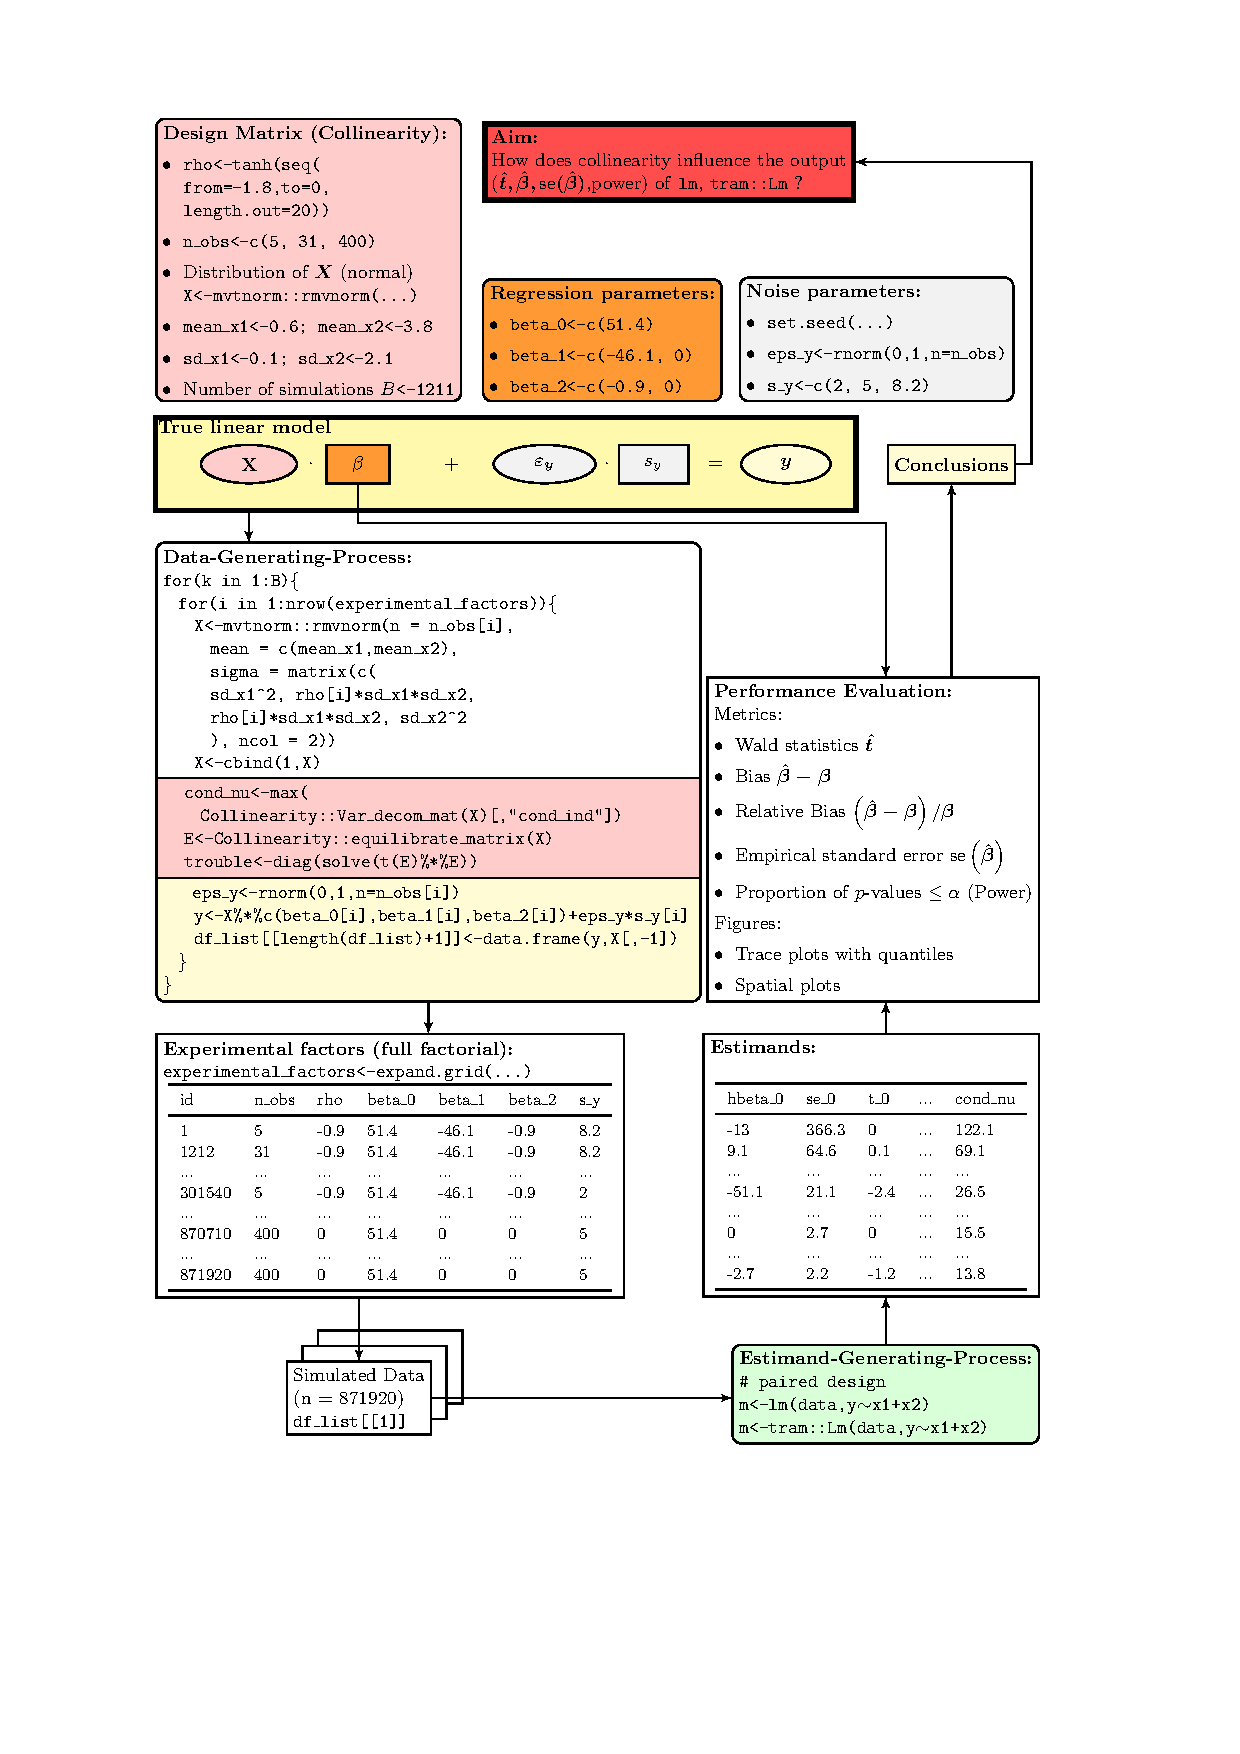
\includegraphics[width=1.2\textwidth]{../sim_workflow_tikz/flow_para}
\vspace*{-50mm}
\caption{Simulation workflow for the parameter estimation process comparing the least squares model \texttt{lm} with the transformation model equivalent \texttt{tram::Lm} with respect to collinearity susceptibility.}
\label{fig:sim_para}
\end{center}
\end{figure}


\newpage
\begin{figure}[H]
\begin{center}
\vspace*{-1cm}
\hspace*{-1cm}
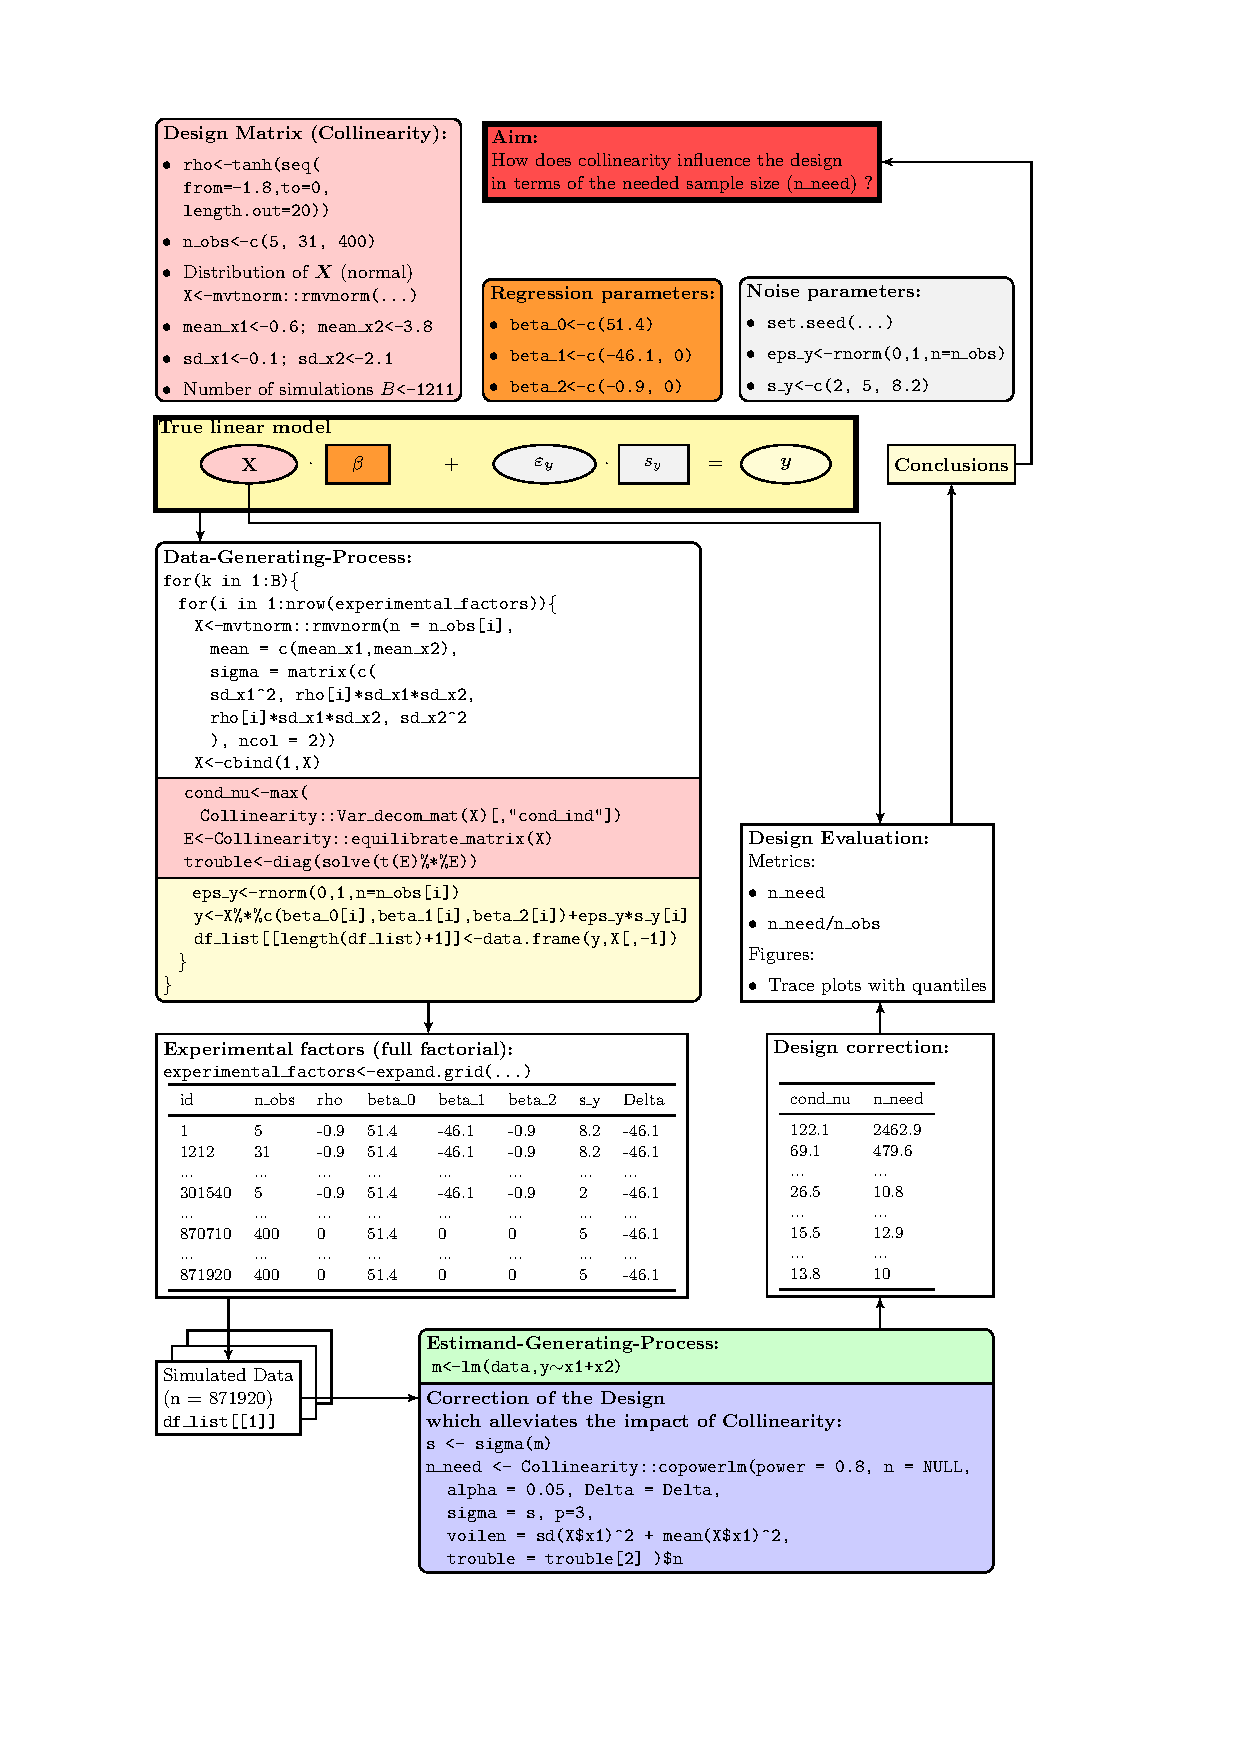
\includegraphics[width=1.2\textwidth]{../sim_workflow_tikz/flow_design}
\vspace*{-30mm}
\caption{Simulation workflow for the design correction through an appropriate sample size that can alleviate the harm caused by collinearity. So far, this procedure only applies for the \texttt{lm} model.}
\label{fig:sim_design}
\end{center}
\end{figure}


%%%%%%%%%%%%%%%%%%%%%%%%%%%%%%%%%%%%%%%%%%%%%%%%%%%%%%%%%%%%%%%%%%%%%%%%%%%%%%%%%
\section{Aim}\label{sec:sim_aim}
%%%%%%%%%%%%%%%%%%%%%%%%%%%%%%%%%%%%%%%%%%%%%%%%%%%%%%%%%%%%%%%%%%%%%%%%%%%%%%%%%

The aim for this particular simulation study is: We want to compare the conventional least-squares model \texttt{lm} with the transformation model equivalent \texttt{tram::Lm} under different collinearity magnitude in the design matrix $\X$. The experimental factors that  change in this simulation are:
\begin{itemize}
\item Magnitude of collinearity (\texttt{rho})
\item Number of observations (\texttt{n\_obs})
\item Magnitude of noise (\texttt{s\_y})
\item Effect and no effect (\texttt{beta\_0, beta\_1, beta\_2})
\end{itemize}

%%%%%%%%%%%%%%%%%%%%%%%%%%%%%%%%%%%%%%%%%%%%%%%%%%%%%%%%%%%%%%%%%%%%%%%%%%%%%%%%%
\section{Data generating process}
%%%%%%%%%%%%%%%%%%%%%%%%%%%%%%%%%%%%%%%%%%%%%%%%%%%%%%%%%%%%%%%%%%%%%%%%%%%%%%%%%

Since this simulation study is inspired by the \texttt{BostonHousing2} data set, we also borrow our parameters for the data generation process from it. We start with generating the collinear design matrix $\boldsymbol{X}\in \R^{\texttt{n\_obs}\times p}$ where $p$ is 3 and \texttt{n\_obs} will be determined later. 

% %%%%%%%%%%%%%%
\subsection{How to generate $\boldsymbol{X}$ with controlled collinearity?}
% %%%%%%%%%%%%%%

In the linear regression setup, we do not make any assumption about the explanatory variables, except that they are measured without error. Thus, we can choose a distribution of our own liking. Of more importance is the magnitude of collinearity within $\X$.
To control collinearity, we considered three options: \textit{scaling factor} (\texttt{scalefactor}) and \textit{multivariate normal method} with transformation to uniform distribution (\texttt{rmvuni}) and without transformation to different distribution (\texttt{rmvnorm}). We follow the approach where we stick with the multivariate normal distribution, but state now all three options for completeness.

%%%%
\subsubsection{Scaling factor (\texttt{scalefactor})}\label{section:scaling}
%%%%

This method is similar to the used approach in \cite{Belsley1991}[Chapter~4], and the idea here is that we start with generating one explanatory variable $\x_1$ as we want and then generate a second explanatory variable $\x_2$ based on $\x_1$ via a linear transformation. The magnitude of collinearity, more specifically correlation, is determined by adding some noise $\bvarepsilon_x$ to $\x_1$. The amount of noise added can be determined by multiplying $\bvarepsilon_x$ with the scaling factor $s_x$. A lot of noise will lead to $\x_1$ and $\x_2$ having less correlation. On the other hand, almost no noise will lead to the fact that $\x_2$ can almost perfectly be described by linear transformations of $\x_1$ and thus leads to high correlation. 

Therefore, we draw \texttt{n\_obs} samples from a uniform distribution whose borders are inspired by the range of \texttt{nox} from the \texttt{BostonHousing2} data set. Thus,
\begin{align}
\x_1\sim \U_{\texttt{n\_obs}}(0.4, 0.9)\label{eq:x_nox}
\end{align}
The second explanatory variable $\x_2$ is generated from $\x_1$ as
\begin{align}
\x_2=\gamma_0 + \gamma_1\cdot \x_1 + \bvarepsilon_x\cdot s_x\label{eq:x_dis}
\end{align}
where $\gamma_0$ and $\gamma_1$ are here leaned on the coefficients obtained by fitting the model \texttt{lm(data = BostonHousing2, dis$\sim$nox)} (Table~\ref{tab:bost_exp}). $\bvarepsilon_x$ is an \texttt{n\_obs}-dimensional vector containing independent and identical draws of the standard normal distribution $\N(0,1)$ and $s_x$ is the scaling factor that allows us to control the magnitude of collinearity. 

\begin{table}[h]
\begin{center}
\caption{Analyzing (weighted) distance of Housings to five employment centers (\texttt{dis}) with simple linear regression via the \texttt{lm} function for the \textit{whole} data set ($n$=506). Outcome variable is the weighted distances to five Boston employment centers (\texttt{dis}). Explanatory variable \texttt{nox} is continuous.}
\label{tab:bost_exp}
% latex table generated in R 4.2.1 by xtable 1.8-4 package
% Tue Nov  8 12:02:32 2022
\begingroup\footnotesize
\begin{tabular}{rrrrr}
  \hline
 & $\hat\gamma$ & 95\% confidence interval & $t$-value & $p$-value \\ 
  \hline
Intercept & 11.55 & from 10.97 to 12.12 & 39.41 & $<$ 0.0001 \\ 
  nox & -13.98 & from -14.99 to -12.96 & -27.03 & $<$ 0.0001 \\ 
   \hline
\end{tabular}
\endgroup

\end{center}
\end{table}

%%%%
\subsubsection{Multivariate normal and transformation to uniform (\texttt{rmvuni})}\label{section:mvt}
%%%%
The second method employs drawing \texttt{n\_obs} samples from a standard multivariate normal distribution with the variance-covariance matrix $\boldsymbol{\Sigma}$ being equivalent to the correlation matrix $\boldsymbol{C}$
\begin{align}
\begin{pmatrix}
  Z_{11} & Z_{12} \\
  \vdots & \vdots \\
  Z_{\texttt{n\_obs}1} & Z_{\texttt{n\_obs}2}
\end{pmatrix}
\sim
\N\left(\boldsymbol{\mu} = \begin{pmatrix}
  0  \\ 0
\end{pmatrix},
\boldsymbol{\Sigma} = \begin{pmatrix}
  1 & \rho_{12} \\
  \rho_{21} & 1
\end{pmatrix}\right)
\label{eq:rmv}
\end{align}
where $\rho_{12}=\rho_{21}$ is the correlation coefficient between realizations $\boldsymbol{z}_1$ and $\boldsymbol{z}_2$ defined between -1 and 1 (and has thus natural bounds, which is good for us with respect to parameter definition for the simulation). Starting from $\boldsymbol{z}_1$ and $\boldsymbol{z}_2$, which are currently standard normal distributed with a certain collinearity, we can generate the distribution we want, by, in a first step, transforming them to be standard uniform distributed using the inverse transformation. If $z_{ij}$ is a realization of a random variable $Z_{ij}$ with cumulative distribution function $F_{Z_{ij}}(z_{ij})$, we can rearrange to 
\begin{align*}
F_{Z_{ij}}(z_{ij})&=\bfP\left(Z_{ij}\leq z_{ij}\right)=\bfP\left(T(U)\leq z_{ij}\right)=\bfP\left(U \leq T^{-1}(z_{ij})\right)
\end{align*}
and when $U$ is standard uniform it holds that $\bfP(U\leq u)=u$ and thus
\begin{align*}
F_{Z_{ij}}(z_{ij})&=T^{-1}(z_{ij})\sim \U(0,1)
\end{align*}
where $F_{Z_{ij}}(z_{ij})$ is in our case $\Phi(z_{ij})$. Thus, $\Phi\left(\boldsymbol{z}_1\right)$ and $\Phi\left(\boldsymbol{z}_2\right)$ are now both standard uniform with a certain correlation and can be further transformed. In our case, we change the support $a_1$ and $b_1$ by
\begin{align*}
\boldsymbol{x}_1 = \Phi\left(\boldsymbol{z}_1\right)\cdot (b_1-a_1) + a_1
\end{align*}
where now $\boldsymbol{x}_1\sim \U_{\texttt{n\_obs}}(a_1=0.4,b_1 = 0.9)$ and the support is leaned on the \texttt{BostonHousing2} data set. The same procedure is also applied to generate the second explanatory variable $\boldsymbol{x}_2$ $(a_2=1.1,b_2 = 12.1)$. Using the uniform distribution has the advantage that we can strictly define the range of our explanatory variables. The disadvantage is that it is not very natural with observations sticking very densely to the corners (Figure~\ref{fig:sim_comp_data}) which might influence the analysis.

%%%%
\subsubsection{Multivariate normal (\texttt{rmvnorm})}\label{section:mvt_stay}
%%%%
The third case that we inspect is if we keep the standard normal distribution, but we shift and scale the data to have the same marginal mean $\mu_{\boldsymbol{x}_1}$ and standard deviation $\sigma_{\boldsymbol{x}_1}$ as the \texttt{BostonHousing2} data set.
Thus, we draw observations described by Equation~\eqref{eq:rmv} and transform them as
\begin{align*}
\boldsymbol{x}_j = \boldsymbol{z}_j\cdot \sigma_{\boldsymbol{x}_j} + \mu_{\boldsymbol{x}_j}
\end{align*}

%%%%
\subsubsection{Collinearity over the correlation matrix}\label{sec:collovercorr}
%%%%
Of course, $\boldsymbol{C}$ describes directly the correlation, which is not exactly collinearity but rather a special case thereof. Furthermore, we invest collinearity on the design matrix $\X$ which includes a constant column of ones ($\boldsymbol{x}_0$) as this can also contribute to collinearity. Nevertheless, there is no angle for us to manipulate on $\boldsymbol{x}_0$ as this is clearly given, which leaves us with $\boldsymbol{x}_1$ and $\boldsymbol{x}_2$ to steer the \textit{whole} amount of collinearity in $\boldsymbol{X}$ and thus operating on $\boldsymbol{C}$ seems to be valid.

Extension of this method to design matrices of higher dimension $p>3$ are of course also possible. As described earlier in Section~\ref{sec:transformX}, when we \textit{standardize} the design matrix and take the square of it, we end up with the correlation matrix $\boldsymbol{C}$ which lacks the constant column.
\begin{align}
\boldsymbol{W^\top W}=\boldsymbol{C}=
\begin{pmatrix}
  1 & \rho_{12} & \ldots & \rho_{1p}\\
  \rho_{21} & 1 & \ldots & \rho_{2p} \\
  \vdots & \vdots & \ddots & \vdots \\
  \rho_{p1} & \rho_{p2} & \ldots & 1\\
\end{pmatrix}\label{eq:corrmat}
\end{align}
Although all individual parameters describe only the \textit{pairwise correlation}, the degree of \textit{collinearity} within $\boldsymbol{W}$ can be determined, as the eigenvalue decomposition works on this scale and the results of the singular value decomposition can approximate these results.
However, the later transformation to the distribution of choice and the addition of the constant column to end up at the design matrix $\X$, will not surprisingly yield a different condition number.
Nevertheless, the transformation and the constant column are independent of the collinearity magnitude which means that the correlation coefficients, $\frac{(p-1)p}{2}$ in number, are still the only parameters that determine the level of \textit{collinearity} within $\X$.

\begin{figure}[H]%H is strict!
\begin{center}
\begin{knitrout}
\definecolor{shadecolor}{rgb}{0.969, 0.969, 0.969}\color{fgcolor}
\includegraphics[width=\maxwidth]{figure/ch05_figcortocl-1} 
\end{knitrout}
\end{center}
\vspace{-1cm}
\caption{Visualization how different correlation coefficients impact collinearity, which is described by the condition number. The condition number is approximated via the eigenvalue decomposition of the correlation matrix $\boldsymbol{C}=\boldsymbol{W^\top W}$ for the 3-dimensional case. For an easier visualization, the condition number is split into 5 bins, where the bin in red represents condition numbers higher then 30.}
\label{fig:cortocol}
\end{figure}

Figure~\ref{fig:cortocol} illustrates for the 3-dimensional case how different constellations of $\rho_{12},\rho_{13}$ and $\rho_{23}$ lead to a rank-deficient, or almost rank-deficient, matrix $\boldsymbol{C}$ expressed by high condition numbers. This figure should emphasize that it is possible to get high collinearity while still having rather low correlation coefficients.

% %%%%%%%%%%%%%%
\subsection{The outcome?}
% %%%%%%%%%%%%%%

When $\X$ is set, we can tackle the outcome variable $\y$. With a column of a ones, our design matrix $\X$ takes the form
\begin{align}
\boldsymbol{X}=
\begin{pmatrix}
  1 & x_{11} & x_{12} \\
  \vdots & \vdots & \vdots \\
  1 & \x_{\texttt{n\_obs}1} & x_{\texttt{n\_obs}2} \\
\end{pmatrix}\in\R^{\texttt{n\_obs}\times 3}\label{eq:desma}
\end{align}

and the outcome $\y$ is then generated as
\begin{align*}
\y=\X\cdot \left(\beta_0,\beta_1,\beta_2\right)^\top
+ \boldsymbol{\varepsilon}_y\cdot s_y
\end{align*}
where $\beta_0, \beta_1$ and $\beta_2$ are inspired by coefficients obtained by fitting the model \\\texttt{lm(data=BostonHousing2, cmedv$\sim$dis+nox)}(Table~\ref{tab:bost_log}). In addition, $\beta_1$ and $\beta_2$ will both have a second experimental condition specified as zero. $\boldsymbol{\varepsilon}_y$ is an \texttt{n\_obs} dimensional vector containing independent and identical draws of the standard normal distribution $\N(0,1)$ and $s_y$ is also a parameter that is inspired by the same fitted model, where it serves as the residual standard error. $s_y$ will also have two additionally different realizations to explore more experimental conditions.

\begin{table}[H]
\begin{center}
\caption{Analyzing Boston Housing prices with multiple linear regression via the \texttt{lm} function for the \textit{whole} data set ($n$=506). Outcome variable is the (corrected) median value of the owner occupied homes in USD 1000 (\texttt{cmedv}). Explanatory variables \texttt{nox} and \texttt{dis} are both continuous.}\label{tab:bost_log}
% latex table generated in R 4.2.1 by xtable 1.8-4 package
% Tue Nov  8 12:02:48 2022
\begingroup\footnotesize
\begin{tabular}{rrrrr}
  \toprule
 & $\hat\beta$ & 95\% confidence interval & $t$-value & $p$-value \\ 
  \midrule
Intercept & 51.38 & from 44.27 to 58.48 & 14.21 & $<$ 0.0001 \\ 
  nox & -46.10 & from -55.81 to -36.38 & -9.32 & $<$ 0.0001 \\ 
  dis & -0.86 & from -1.40 to -0.33 & -3.18 & 0.002 \\ 
   \bottomrule
\end{tabular}
\endgroup

\end{center}
\end{table}

Thus according to Table~\ref{tab:bost_log}, after having specified $\X$, the following parameters are set to create the outcome $\y$:
\begin{multicols}{2}
\begin{itemize}
\item $\beta_0$ ($\beta_\texttt{Intercept}$) set as \texttt{c(51.4)}
\item $\beta_1$ ($\beta_\texttt{nox}$) set as \texttt{c(-46.1, 0)}
\item $\beta_2$ ($\beta_\texttt{dis}$) set as \texttt{c(-0.9, 0)}
\item $s_y$ set as \texttt{c(2, 5, 8.2)})
\end{itemize}
\end{multicols}

where all these parameter are rounded on one decimal place.

%%%%
\newpage
\subsection{Comparison of methods}
%%%%

We create 50 collinearity situations of different magnitude and for each of these situations we create 100 data sets consisting of 500 observations. There is not really a rationale for these parameters, but should only visualize the different data properties each method is accompanied by. Although $\beta_1, \beta_2$ and $s_y$ have several conditions, all of them take in this example the realization that is inherited from the \texttt{BostonHousing2} data set: $\beta_1=-46.1$, $\beta_2=-0.9$, $s_y=8.2$.

The individual data frames are generated as described earlier in this section. $\rho$ is iterated on an equally spaced grid between 0 and -1. The negative correlation is chosen because as visible in Table~\ref{tab:bost_exp} the association between variable $\x_1$ (\texttt{nox}) and $\x_2$ (\texttt{dis}) is negative ($\gamma_\texttt{nox}$=-14).

For the \texttt{scalefactor} method, the grid for $s_x$ is determined by computing the scale factors that are needed to achieve the same minimum and maximum condition number, the \texttt{rmvuni} method could achieve. These borders are determined by a uniroot function and $s_x$ is iterated between these two borders with an equal spacing.

Furthermore, the outcome variable $\y$ is also generated and subsequently the least-squares linear model \texttt{lm(y$\sim$x1+x2)} is fitted to figure out whether the different simulation methods also end up with different results. The transformation model equivalent is not yet applied, as we are currently only comparing the data generation process.

Figure~\ref{fig:sim_comp} plots on the first two rows the diagonal entries of $\left(\boldsymbol{E^\top E}\right)^{-1}$ versus the correlation coefficient $\rho$, the condition number $\kappa\left(\boldsymbol{E}\right)$ respectively. The third row visualizes the correlation coefficient versus the condition number, and it seems to be the case that for the same condition number, the correlation is highest in the \texttt{rmvnorm} method. This effect seems to be more pronounced for lower condition numbers.

The fourth row plots the standard deviation of the explanatory variables.
This row crystallizes the difference when simulating with the \texttt{scalefactor} or drawing from the multivariate normal (\texttt{rmvnorm} or \texttt{rmvuni}): Variable $\x_2$ (\texttt{dis}) that is constructed from $\x_1$ (\texttt{nox}) has a non-constant standard deviation, as this is the parameter that defines the collinearity within $\X$.
The standard deviation for $\x_1$ in the \texttt{scalefactor} method stays horizontally the same, as the collinearity magnitude is only defined by $s_x$ but works with the same random pattern. This means that there are only 100 different random patterns, and each of them is 50 times scaled to get different collinearity situations. Thus, the \texttt{scalefactor} method yields dependent data sets, whereas for \texttt{rmvnorm} and \texttt{rmvuni}, all generated data sets are independent of each other.

The three last rows show the estimated coefficients $\hbbeta[i,j]$, the standard error $\se\left(\hbbeta[i,j]\right)$ and the Wald-Statistics $\hbt[i,j]$ for all created data sets. It seems to be the case that the non-constant standard deviation for $\boldsymbol{x}_2$ that accompanies the \texttt{scalefactor} method, has an effect on all three statistics.
Thus, all three methods will cause different estimation behavior, but whether one of them is better or worse is not clear.



\newpage

\begin{figure}[H]%H is strict!
\begin{center}
\begin{knitrout}
\definecolor{shadecolor}{rgb}{0.969, 0.969, 0.969}\color{fgcolor}
\includegraphics[width=\maxwidth]{figure/ch05_figsim_comp-1} 
\end{knitrout}
\end{center}
\vspace{-1cm}
\caption{Comparing \texttt{rmvuni, rmvnorm} and \texttt{scalefactor} approaches to induce collinearity.}
\label{fig:sim_comp}
\end{figure}

\newpage

Figure~\ref{fig:sim_comp_data} compares how the \textit{raw} data for two different collinearity magnitudes differs between the simulation approaches. We see here even clearer that the \texttt{scalefactor} method (blue) does not protect the marginal standard deviation of $\x_2$ (\texttt{dis}) whereas the multivariate normal method does. In addition, we see that for \texttt{rmvuni}, the borders are respected but we see that the observations are preferably scattered at the upper-left and lower-left corner which seems not very natural.

\begin{figure}[H]%H is strict!
\begin{center}
\begin{knitrout}
\definecolor{shadecolor}{rgb}{0.969, 0.969, 0.969}\color{fgcolor}
\includegraphics[width=\maxwidth]{figure/ch05_figsim_comp_data-1} 
\end{knitrout}
\end{center}
\vspace{-1.2cm}
\caption{Comparing approaches to induce collinearity. Visualization how the two variables $\boldsymbol{x}_1$ and $\boldsymbol{x}_2$ are in relation to each other for the different methods but for somewhat similar collinearity magnitudes. The black dot and the dotted lines represents the location of the mean and range of the two explanatory variables coming from the \texttt{BostonHousing2} data set.}
\label{fig:sim_comp_data}
\end{figure}

To summarize a few points to compare the methods:
\begin{enumerate}
\item \textit{Dependency}: Whereas the \texttt{scalefactor} method may have dependent data sets, and thus also dependent estimates, \texttt{rmvuni} and \texttt{rmvnorm} break this association.
\item \textit{Marginal standard deviation}: The \texttt{scalefactor} method results in different standard deviations for $\boldsymbol{x}_2$ depending on the collinearity magnitude. The \texttt{rmvuni} and \texttt{rmvnorm} methods protect the marginal standard deviation of the created variables.
\item \textit{Range}: In the \texttt{rmvuni} and \texttt{rmvnorm} methods we induce collinearity over the correlation matrix $\boldsymbol{C}$ whose coefficients are naturally bounded by $\left(-1,1\right)$. Determining the boundaries for the \texttt{scalefactor} method is less restrictive and setting reasonable limits is a task that might cause serious headache.
\end{enumerate}

Simulation of controlled collinearity for the case when more than two explanatory variables need definition might be more intuitive with the \texttt{scalefactor} method, as one variable can be rather clearly defined by a linear transformation of others.
On the other hand, with this approach one is rather bounded to the case one is imagining and moves a bit away from the more general application.
The dependency is lost when simulating over the \texttt{rmvuni} or \texttt{rmvnorm} method. But this is not necessarily a bad thing, as this simplifies later analysis by not having to correct for dependent estimates.
Of course, breaking the dependency is also possible for the \texttt{scalefactor} method. Nevertheless, with respect to simulation, a clear defined range seems to be very convenient and also a constant marginal standard deviation of the explanatory variables is desirable as this might lead to unexpected effects.
Unexpected effects might be also caused by the transformation to uniform scale (\texttt{rmvuni}), as the points prefer to stick in the corners.

In the end, we conclude that there is not really one optimal method to induce collinearity.
The method we choose to go along with is the \texttt{rmvnorm} method.
With this method, we do not restrict $\X$ to be within the range of the \texttt{BostonHousing} data set, but we don't see this as problematic.
This method seems for us the most convenient and natural method to simulate collinear explanatory variables, and therefore we move along with it.

% %%%%%%%%%%%%%%
\subsection{Sample size \texttt{n\_obs} for continuous variable of interest}
% %%%%%%%%%%%%%%

\texttt{n\_obs} is chosen to be able to find the effect corresponding to variable $\x_1$ (=\texttt{nox}) with a power of 80\% and significance level of $\alpha=$0.05 when \textit{no} collinearity is assumed. Even though we change the magnitude of collinearity within the simulation, \texttt{n\_obs} stays constant throughout the whole simulation to point out the effect solely caused by collinearity. To determine the sample size \texttt{n\_obs} we employ the function \texttt{Collinearity::copowerlm} with the parameters defined earlier employed at the noisiest condition specified at the maximum \texttt{s\_y} value as:
\begin{multicols}{2}
\begin{itemize}
\item \texttt{power}=0.80
\item \texttt{n}=NULL
\item \texttt{alpha}=0.05
\item \texttt{Delta}=$\beta_1$=-46.1
\item \texttt{sigma}=$s_y$=8.2
\item \texttt{p}=3
\item \texttt{voilen}=$\var(X_1)+\E(X_1)^2$=0.443
\item \texttt{trouble}=\dots
\end{itemize}
\end{multicols}
where a crucial parameter is \texttt{trouble} is yet missing. \texttt{trouble} is still the diagonal entry of $\left[\left(\boldsymbol{E^\top E}\right)^{-1}\right]$ corresponding to $\beta_1$ and assumed to be 1 with no collinearity if we equilibrate the design matrix $\boldsymbol{X}$. This will almost never be the case, even if we construct $\boldsymbol{X}$ to have as less collinearity as we can. 

This is hardly visible in Figure~\ref{fig:sim_comp} due to the scale  but the Diagonal Entry never reaches 1 in the case where we simulate collinearity with the multivariate normal distribution. Figure~\ref{fig:real_trouble} zooms in and makes this clearer.

\begin{figure}[h]%H is strict!
\begin{center}
\begin{knitrout}
\definecolor{shadecolor}{rgb}{0.969, 0.969, 0.969}\color{fgcolor}
\includegraphics[width=\maxwidth]{figure/ch05_figreal_trouble_plot-1} 
\end{knitrout}
\end{center}
\vspace{-1cm}
\caption{Visualization of the dynamic of the diagonal entries and a cross-section at $\rho=0$, represented by the histograms. In addition, the 2.5\%, 50\%, 97.5\% quantiles are plotted as well.}
\label{fig:real_trouble}
\end{figure}
\vspace{-0.4cm}
To get an even clearer picture about the distribution of the diagonal entries (\texttt{trouble}) at the point where the collinearity within $\boldsymbol{X}$ should be lowest, ($\rho=0$) we draw 200 data sets, each containing 500 observations. Then we calculate the diagonal entries of $\left(\boldsymbol{E^\top E}\right)^{-1}$, plot it with a histogram for each variable separately and also add the 2.5\%, 50\% and 97.5\% quantiles (Figure~\ref{fig:real_trouble}
). We see that even though we construct $\boldsymbol{X}$ as good as we can to have no collinearity and thus would mean that the diagonal entries of $\left(\boldsymbol{E^\top E}\right)^{-1}$ are equal to 1, this is simply not the case. 




A sample size, calculated with \texttt{trouble} equals to 1, would yield \texttt{n\_obs} to be 5 (rounded up to the next integer).
If we set \texttt{trouble} to the 97.5\% quantile, which is $\approx$42.581, we get a sample size of 31.
This then covers 97.5\% of all cases when the collinearity is as low as possible. 

To see what happens to the estimates with different sample sizes, we add as sample size levels 5 and an over-powered case with 400 which corresponds to the sample size of 31 times 10 rounded up to the next hundred.
Thus, this means throughout the simulation we have three different levels as \texttt{n\_obs<-c(5, 31, 400)}.

% % %%%%%%%%
\subsection{Range and grid of the collinearity magnitude}
% % %%%%%%%%




Since we have chosen to simulate collinearity over the correlation matrix, defining the range of \texttt{rho} is easy: (-1,0). The negative correlation is chosen because the relation between $\boldsymbol{x}_1$ and $\boldsymbol{x}_2$ is negative too (Table~\ref{tab:bost_exp}). This results in this setup in a condition number range of (13.542, 126.872).

So far, we explored the different collinearity magnitudes with an equal spaced grid on the correlation level (\texttt{rho<-seq(from=-1,to=0,length.out=no\_coll\_magnitude)}), where the number of different correlation levels is 50 (\texttt{no\_coll\_magnitude}).
But the relation between correlation and condition number is of course not linear, leading to the fact that the condition number grid is not explored by even steps, which is visible in Figure~\ref{fig:corcond}. 
\begin{figure}[H]%H is strict!
\begin{center}
\begin{knitrout}
\definecolor{shadecolor}{rgb}{0.969, 0.969, 0.969}\color{fgcolor}
\includegraphics[width=\maxwidth]{figure/ch05_figcorcond-1} 
\end{knitrout}
\end{center}
\vspace{-0.8cm}
\caption{Visualization how the correlation translates into the condition number for one run.}
\label{fig:corcond}
\end{figure}
This is a bit unfortunate as we also want to explore higher collinearity magnitudes. But we can solve this issue with the Fisher transformation (\cite{Fisher1915}) since it is used to transform highly skewed correlation coefficients $\rho$ to be approximately normally distributed. By doing this, one can compute reliable statistics of $\rho$ and of course we can use this transformation for our situation to explore higher condition numbers at a finer grid.
\begin{figure}[H]%H is strict!
\begin{center}
\begin{knitrout}
\definecolor{shadecolor}{rgb}{0.969, 0.969, 0.969}\color{fgcolor}
\includegraphics[width=\maxwidth]{figure/ch05_figfisher_trans-1} 
\end{knitrout}
\end{center}
\vspace{-0.8cm}
\caption{For 1000 \textit{Fisher transformed rho} (\texttt{z}) on a grid between -4 and 0, the transformation to $\boldsymbol{X}$, via the correlation coefficient $\rho$ is simulated. Each $\boldsymbol{X}$ contains 500 observations and the condition number is calculated with the function \texttt{Collinearity::Var\_decom\_mat(X)}.}
\label{fig:fisher_trans}
\end{figure}

The Fisher transformation, which is essentially the inverse hyperbolic tangent function (\texttt{z<-atanh(rho)}), maps $\rho$ which is defined within $[-1,1]$ onto $(-\infty, \infty)$. This means we lose the lower boundary of -1 and thus have to determine it. We do this by setting the proportion of condition numbers, larger than Belsley's cut-off value of 30, to be $1/3$ and determine the maximum \textit{Fisher transformed rho} (\texttt{z}) to achieve this. Figure~\ref{fig:fisher_trans} iterates \texttt{z} on an equally-spaced grid between -4 and 0 for 1000 different values. Then the back-transformation to \texttt{rho} is applied (\texttt{rho<-tanh(z)}) and $\boldsymbol{X}$ is constructed, each having 500 observations. Then the condition number for $\boldsymbol{X}$ is calculated.
The proportion of condition numbers that are higher or equal to 30 are visualized on the upper-right panel and we see that we need the lower limit of the \textit{Fisher transformed rho} (\texttt{z}) to be $\approx$-1.8 to get the desired proportion of $1/3$. Furthermore, the number of different collinearity magnitudes (\texttt{no\_coll\_magnitude}) does not have to be very large, also for computational reasons, and thus we set it to 20. 

Thus, to summarize, the collinearity magnitude in the simulation study will be explored with:
\texttt{rho <- tanh(seq(from=lower\_fisher\_rho,to = 0, length.out = no\_coll\_magnitude))}\\
where \texttt{lower\_fisher\_rho}=-1.8 and \texttt{no\_coll\_magnitude}=20.
Table~\ref{tab:rho} visualizes the translation from the \textit{Fisher transformed rho} (\texttt{z}) to the condition number via the rho corresponding to the correlation coefficient ($\rho$).

\begin{table}[H]\begin{center}
\caption{Visualization how an equally binned \textit{Fisher transformed rho} (\texttt{z}) translates into rho on the correlation level scale ($\rho$) and then into the condition number ($\kappa\left(\boldsymbol{E}\right)$). Note that rho ($\rho$) is only the theoretically assigned for the simulation and deviates to some extent from the actual rho ($\hat\rho$) in the simulated data.}\label{tab:rho}
% latex table generated in R 4.2.2 by xtable 1.8-4 package
% Fri Jan 27 11:59:31 2023
\begingroup\footnotesize
\begin{tabular}{llllll}
  \toprule
Fisher transformed rho (z) &  & rho ($\rho$) &  & rho after sim. ($\hat\rho$) & $\kappa\left(\boldsymbol{E}\right)$ \\ 
  \midrule
-1.8 &  & -0.947 &  & -0.949 & 51.33 \\ 
  -1.6 & 0.2 & -0.922 & 0.025 & -0.91 & 42.077 \\ 
  -1.4 & 0.2 & -0.885 & 0.036 & -0.872 & 36.17 \\ 
  -1.2 & 0.2 & -0.834 & 0.052 & -0.844 & 30.765 \\ 
  -1 & 0.2 & -0.762 & 0.072 & -0.782 & 25.334 \\ 
  -0.8 & 0.2 & -0.664 & 0.098 & -0.688 & 21.902 \\ 
  -0.6 & 0.2 & -0.537 & 0.127 & -0.524 & 18.681 \\ 
  -0.4 & 0.2 & -0.38 & 0.157 & -0.356 & 15.885 \\ 
  -0.2 & 0.2 & -0.197 & 0.183 & -0.157 & 15.469 \\ 
  0 & 0.2 & 0 & 0.197 & 0.072 & 14.768 \\ 
   \bottomrule
\end{tabular}
\endgroup

\end{center}\end{table}





%%%%%%%%%%%%%%%%%%%%%%%%%%%%%%%%%%%%%%%%%%%%%%%%%%%%%%%%%%%%%%%%%%%%%%%%%%%%%%%%%
\section{Estimands}
%%%%%%%%%%%%%%%%%%%%%%%%%%%%%%%%%%%%%%%%%%%%%%%%%%%%%%%%%%%%%%%%%%%%%%%%%%%%%%%%%

The estimands considered are the coefficients $\hbbeta[i,j]$, standard error $\se\left(\hbbeta[i,j]\right)$ and the Wald statistics $\hbt[i,j]=\frac{\hbbeta[i,j]}{\se\left(\hbbeta[i,j]\right)}$ for the explanatory variables not including the intercept though.

%%%%%%%%%%%%%%%%%%%%%%%%%%%%%%%%%%%%%%%%%%%%%%%%%%%%%%%%%%%%%%%%%%%%%%%%%%%%%%%%%
\section{Sample size needed}
%%%%%%%%%%%%%%%%%%%%%%%%%%%%%%%%%%%%%%%%%%%%%%%%%%%%%%%%%%%%%%%%%%%%%%%%%%%%%%%%%

A further measure that is related to the design of the study is the number of observations needed to reach the desired power of 80\% given the current collinearity magnitude.
We call this measure \texttt{n\_need}, and it is determined with the \texttt{copowerlm} function of the \texttt{Collinearity} package \citep{Collinearity}. 
As \texttt{copowerlm} is developed to be applicable for the least-squares case and thus is only applied to determine the needed sample size based on results that are fitted with the \texttt{lm} function.

\texttt{copowerlm} can be used as a tool to  determine the appropriate sample size to have a power of 80\% corresponding to a certain variable of interest.
This function extends already existing sample size software as it takes the collinearity information within the model into consideration and adjusts for that.

%%%%%%%%%%%%%%%%%%%%%%%%%%%%%%%%%%%%%%%%%%%%%%%%%%%%%%%%%%%%%%%%%%%%%%%%%%%%%%%%%
\section{Methods}
%%%%%%%%%%%%%%%%%%%%%%%%%%%%%%%%%%%%%%%%%%%%%%%%%%%%%%%%%%%%%%%%%%%%%%%%%%%%%%%%%
Multiple linear regression methods:
\begin{itemize}
\item \texttt{lm(\dots)}
\item \texttt{tram::Lm(\dots)}
\end{itemize}
Methods are employed at their default parameters.

%%%%%%%%%%%%%%%%%%%%%%%%%%%%%%%%%%%%%%%%%%%%%%%%%%%%%%%%%%%%%%%%%%%%%%%%%%%%%%%%%
\section{Performance measures}\label{sec:performance}
%%%%%%%%%%%%%%%%%%%%%%%%%%%%%%%%%%%%%%%%%%%%%%%%%%%%%%%%%%%%%%%%%%%%%%%%%%%%%%%%%
The distribution of the following performance measures is inspected graphically via plotting the trace of the estimands along the condition number grid. The trace means that we compute percentiles (5\%, 25\%, 50\%, 75\%, 95\%) for a specific condition number to get an idea about the distribution of the estimand.
To have meaningfully computed percentiles, we need to have a certain amount of observations.
Thus, we employ some sort of \textit{moving quantile} method, where we condense 100 observations into one and calculate the quantiles plus the median condition number for this particular window.
Then one moves along by dropping the first 10 observations but adds the next 10 and performs the same computation again.
This procedure is then done until one has moved the window through the whole data set.
\begin{itemize}
\item Both statistical methods not comparable:
  \begin{itemize}
  \item Trace of the estimated coefficient $\hbbeta[i,j]$
  \item Trace of the standard error $\se\left(\hbbeta[i,j]\right)$
  \item Trace of the bias $\E\left(\hbbeta[i,j]\right)-\bbeta[j]$
  \end{itemize}
\item Both statistical methods comparable:
  \begin{itemize}
  \item Trace of the Wald statistics $\hbt[i,j]$ 
  \item Trace of the relative bias $\left(\frac{\E\left(\hbbeta[i,j]\right)-\bbeta[j]}{\bbeta[j]}\right)$
  \item Proportion of $p$-values $\leq\alpha=0.05$ plus discriminating whether the estimate has a correct or incorrect sign and thus is correctly or incorrectly significant
  \end{itemize}
\item Plotting the Wald statistics of \texttt{tram::Lm} minus the \texttt{lm} model on the $y$-axis versus the condition number on the $x$-axis.
\item Plotting the Wald statistics of the \texttt{tram::Lm} model on the $y$-axis versus the Wald statistics of the \texttt{lm} model on the $x$-axis.
\item Plotting the Wald statistics of \texttt{tram::Lm} minus the \texttt{lm} model on the $y$-axis versus the Wald statistics of the \texttt{lm} model on the $x$-axis
\end{itemize}

%%%%%%%%%%%%%%%%%%%%%%%%%%%%%%%%%%%%%%%%%%%%%%%%%%%%%%%%%%%%%%%%%%%%%%%%%%%%%%%%%
\section{Determining the number of simulations}\label{sec:B}
%%%%%%%%%%%%%%%%%%%%%%%%%%%%%%%%%%%%%%%%%%%%%%%%%%%%%%%%%%%%%%%%%%%%%%%%%%%%%%%%%

According to \cite{Burton2006}, the determination of the number of simulations to be performed ($B$) \textit{can} be based on the accuracy of the estimate of interest. One can make a sample size calculation based on the (1-$\alpha$)\% confidence interval with a \textit{fixed width}. Thus, the (1-$\alpha$)\% confidence interval for $\bar{\hat{t}}$ is 
\begin{align*}
\bar{\hat{t}}\pm Z_{1-(\alpha/2)}\cdot \se\left(\bar{\hat{t}}\right)
\end{align*}
with standard error being
\begin{align*}
\se\left(\bar{\hat{t}}\right) &=\sqrt{\var\left(\frac{1}{B}\sum_{i=1}^{B}\hbt[i]\right)}=\sqrt{\frac{1}{B} \var\left(\hbt[i]\right) }=\frac{\sqrt{\var\left(\hbt[i]\right) }
}{\sqrt{B}}
\end{align*}
The half width of the confidence interval, which we call $\delta$, is then
\begin{align*}
\delta&=Z_{1-(\alpha/2)}\cdot \frac{\sqrt{\var\left(\hbt[i]\right) }
}{\sqrt{B}}
\end{align*}
which can then be solved for $B$
\begin{align}
B&=\left(\frac{Z_{1-(\alpha/2)}\cdot \sqrt{\var\left(\hbt[i]\right) }
}{\delta}\right)^2
\label{eq:ss_B}\end{align}



The half-width $\delta$ is the pre-specified level of accuracy for the estimate of interest, which is in our case the Wald-statistics $\hbt[i]$ corresponding to the variable of interest. $\delta$ means the largest difference $|\hbt[i]-\t[i]|$ one is willing to accept, and we take here 0.1 as reasonable.

$\sqrt{\var\left(\hbt[i]\right) }$ is the variance of $\hbt[i]$ and is determined by an initial small run employed at the worst condition, which is the situation with the highest collinearity magnitude that we are going to inspect as $\kappa\left(\boldsymbol{E}\right)=60$ and with the noisiest and in-stable data specified with \texttt{s\_y}=8.2 and \texttt{n}=5.
Due to the instability, the resulting condition numbers vary quite heavily, and thus we simulate data with a \texttt{while} loop and only take the realizations where a condition number rounded to full digits is equal to 60 and continue the loop until we have 100 $\hbt[i]$ values.
Thus, we employ Equation~\eqref{eq:ss_B} with $\alpha=0.05$, $\delta$=0.1 and $\sqrt{\var\left(\hbt[i]\right) }$=1.775 which yields $B\approx$1211.


%%%%%%%%%%%%%%%%%%%%%%%%%%%%%%%%%%%%%%%%%%%%%%%%%%%%%%%%%%%%%%%%%%%%%%%%%%%%%%%%%
\section{Handling exceptions}\label{sec:sim_exceptions}
%%%%%%%%%%%%%%%%%%%%%%%%%%%%%%%%%%%%%%%%%%%%%%%%%%%%%%%%%%%%%%%%%%%%%%%%%%%%%%%%%

When running the estimation methods, errors and warnings will be caught with NA values and the resulting output from the method will be considered unreasonable and thus will be missing. The cause of the issues will not be explicitly examined. Investigating any occurring exceptions will be facilitated since we store the random seed before each simulation run.










%%%%%%%%%%%%%%%%%%%%%%%%%%%%%%%%%%%%%%%%%%%%%%%%%%%%%%%%%%%%%%%%%%%%%%


% LaTeX file for Chapter 06


%%%%%%%%%%%%%%%%%%%%%%%%%%%%%%%%%%%%%%%%%%%%%%%%%%%%%%%%%%%%%%%%%%%%%%%%%%%%%%%%
\chapter{Results: Simulation study}\label{results}
%%%%%%%%%%%%%%%%%%%%%%%%%%%%%%%%%%%%%%%%%%%%%%%%%%%%%%%%%%%%%%%%%%%%%%%%%%%%%%%%



This chapter provides the results of the simulation study developed in Section~\ref{simstudy}. Only for \texttt{n\_need} aspect of the simulation 4 out of 871920 experimental conditions yield NA values that were not expected, and thus we will not further investigate these issues. The simulation was executed with only one core and took approximately 11.8 hours to run.
This process can be accelerated using parallelized computing. An example of how to do this is provided in the file (\url{https://bitbucket.org/jsepin/simulation/src/master/simulation_total.R}) with the commented-out simulation.

For example, this simulation can be performed in approximately 50 minutes when using 64 cores.
However, we did not use parallelized computing as the results also depend on how many cores are at work and thus depending on the resources available, not everyone may be able to reproduce the results in this master thesis.

This report focuses only on two experimental conditions $\beta_1=-46.1,\beta_2=-0.9$ and $\beta_1=0,\beta_2=0$ and three estimands, namely the Wald statistics, proportion of significant results, and \texttt{n\_need}.
This is because the Wald statistics represents the most important estimand which quantifies what we define as harmful.
All remaining results are provided online (\url{https://bitbucket.org/jsepin/simulation/src/master/results_simulation/results_simulation.pdf}).

%%%%%%%%%%%%%%%%%%%%%%%%%%%%%%%%%%%%%%%%%%%%%%%%%%%%%%%%%%%%%%%%%%%%%%%%%%%%%%%%%
\section{Performance evaluation of the most important estimands}
%%%%%%%%%%%%%%%%%%%%%%%%%%%%%%%%%%%%%%%%%%%%%%%%%%%%%%%%%%%%%%%%%%%%%%%%%%%%%%%%%
Figures~\ref{fig:simres_wald1} and \ref{fig:simres_wald2} show on the $y$-axis the Wald statistics and on the $x$-axis the condition number for both, \texttt{lm} and \texttt{tram::Lm}.
The condition number ranges between 0 and 60.
The quantiles that are obtained by the moving quantile procedure (Section~\ref{sec:performance}) summarize the distribution of Wald statistics values.
Due to two-sided hypothesis testing, points laying inside (-1.96, 1.96) are interpreted as non-significant and colored as a red area.
Points laying in the white area are said to be significant and with an effect estimate that is negative, which is correct. On the other hand, Wald statistic values in the yellow area are thought to be significant, but the sign of the effect is positive and thus wrong.
In Figure~\ref{fig:simres_wald1}, where we have a true signal ($\beta_1=-46.1,\beta_2=-0.9$), we see that with higher collinearity, quantified by the condition number, Wald statistics move more and more into the red area, resulting in a non-detection. This tendency is the same for both \texttt{lm} and \texttt{tram::Lm} but is even more pronounced for higher noise \texttt{s\_y} and low sample sizes \texttt{n\_obs}. What we also see is that the tendency to have points laying in the yellow area is increased with low sample size and high noise. 
This problem gets even better visible in Figure~\ref{fig:simres_wald2} where there is no signal ($\beta_1=0,\beta_2=0$).
In this figure, the Wald statistics distribution stays quite constant over the whole range of the condition number. But, with lower sample size and higher noise, more points lay outside the red area.

Figures~\ref{fig:simres_differencevscondu1} and \ref{fig:simres_differencevscondu2} plot the Wald statistic differences against the condition number which is possible due to the paired design.
It gets visible that with higher condition number, the difference gets smaller.
The difference seems to increase however with less noise of the data (\texttt{s\_y}), and the difference appears more consistent with increasing sample sizes.

Figures~\ref{fig:simres_prop1} and \ref{fig:simres_prop2} elaborate on the correct and incorrect proportion of significant results. We see here as well that with higher noise, lower sample size and higher collinearity, the proportion of correct significant results decreases. In addition, we note here that as the proportion of correct results decreases, the proportion of incorrect significant results increases.
And further, the figures indicate that \texttt{tram::Lm} has either way more the tendency to have significant results.

Figures~\ref{fig:simres_bivar1} and \ref{fig:simres_bivar2} compare the Wald statistics of \texttt{lm} and \texttt{tram::Lm} as a ratio. 
If both methods yield the same Wald statistics, points would lay on the red line, which is a straight line with a slope of 1.
But, we see that the Wald statistics of \texttt{lm} tends to be much larger than for \texttt{tram::Lm}.

Figures~\ref{fig:simres_differencevslm1} and \ref{fig:simres_differencevslm2} also compare the Wald statistics but as a difference and not as a ratio and plots this difference against the Wald statistics of the \texttt{lm} method.
This means that if Wald statistics values are the same, points would lay on the horizontal line at $y=0$.
Similarly to Figures~\ref{fig:simres_bivar1} and \ref{fig:simres_bivar2} we note that \texttt{lm} tends in general to have much larger Wald statistics values than \texttt{tram::Lm}.
But this effect seems to be inverted for Wald statistics of lower magnitude, and therefore leads to the fact that \texttt{tram::Lm} has more frequently results that are interpreted as significant.
To make this even clearer, the area where \texttt{lm} and  \texttt{tram::Lm} would have Wald statistics values that are interpreted differently in terms of significance is colored in blue. This represents the area between:
\begin{itemize}
\item For $\hat{t}_\text{lm}<0$: $-q_{1-\alpha/2,Z}(\approx 1.96)$ and the function $f(\hat{t}_\text{lm})=-q_{1-\alpha/2,Z} -\hat{t}_\text{lm}$
\item For $\hat{t}_\text{lm}>0$: $\textcolor{white}{-}q_{1-\alpha/2,Z}(\approx 1.96)$ and the function $f(\hat{t}_\text{lm})=\textcolor{white}{-}q_{1-\alpha/2,Z} -\hat{t}_\text{lm}$
\end{itemize}
Since the differences are only in the lower-left and upper-right area, they are interpreted as the zone where \texttt{lm} would not have significant conclusions but \texttt{tram::Lm} does.
However, it seems to be the case that with higher sample sizes, the difference in Wald statistics values vanishes. This behavior appears to be very similar for both conditions of $\beta_1$.


%%%%%%%%%%%%%%%%%%%%%%%%%%%%%%%%%%%%%%%%%%%%%%%%%%%%%%%%%%%%%%%%%%%%%%%%%%%%%%%%
%\vfill
\newpage
\subsection{Wald statistics: $\beta_1=-46.1$ and $\beta_2=-0.9$}
%%%%%%%%%%%%%%%%%%%%%%%%%%%%%%%%%%%%%%%%%%%%%%%%%%%%%%%%%%%%%%%%%%%%%%%%%%%%%%%%%
\begin{figure}[H]
\centering
\begin{subfigure}[b]{1\textwidth}
\vspace*{-0.5cm}
\centering
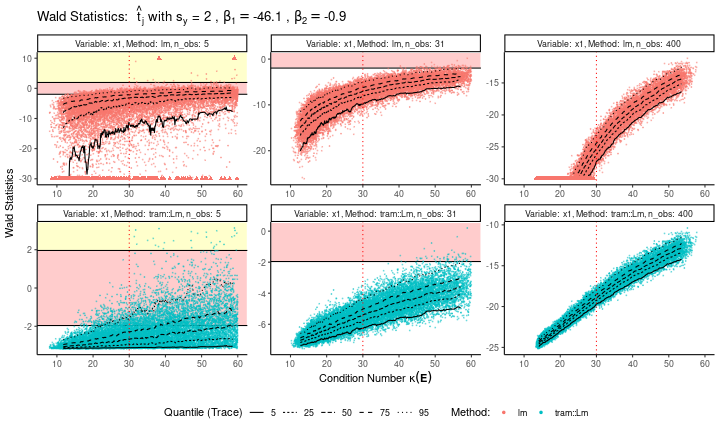
\includegraphics[width=0.85\textwidth]{../fromsim/simres_wald11-1.png}
\end{subfigure}
\begin{subfigure}[b]{1\textwidth}
\vspace*{-0.9cm}
\centering
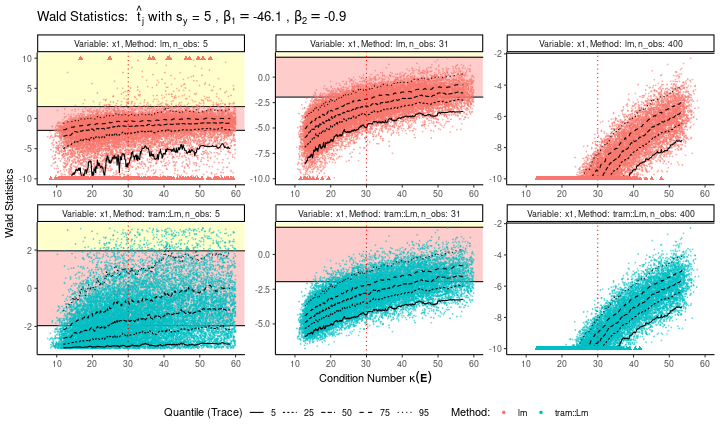
\includegraphics[width=0.85\textwidth]{../fromsim/simres_wald21-1.png}
\end{subfigure}
\begin{subfigure}[b]{1\textwidth}
\vspace*{-0.9cm}
\centering
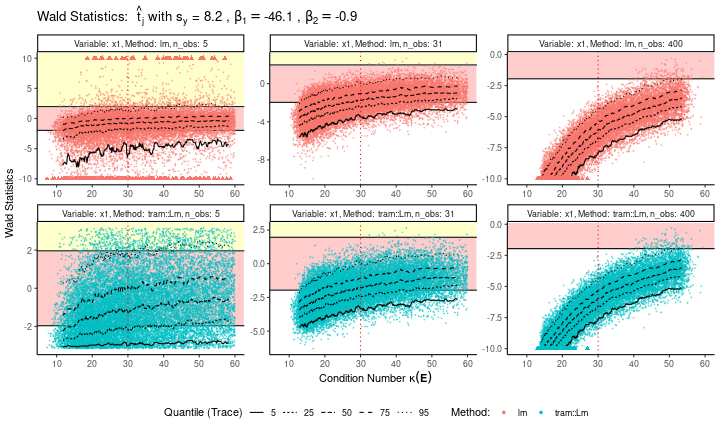
\includegraphics[width=0.85\textwidth]{../fromsim/simres_wald31-1.png}
\end{subfigure}
\vspace*{-1cm}
\caption{Wald statistics versus the condition number. The red shaded area represents Wald statistics between -1.96 and 1.96 which are non-detected signals and thus harmful. Points in the yellow shaded area are even more troublesome since they mean there is a detection, but the signal is incorrect. The frame of the plots are restricted to have maximum $y$-axis range between -10 and 10. Points laying outside are placed at the border and visualized as triangles.}
\label{fig:simres_wald1}
\end{figure}
%%%%%%%%%%%%%%%%%%%%%%%%%%%%%%%%%%%%%%%%%%%%%%%%%%%%%%%%%%%%%%%%%%%%%%%%%%%%%%%%
%\newpage
\vspace*{-1cm}
\subsection{Wald statistics: $\beta_1=0$ and $\beta_2=0$}
%%%%%%%%%%%%%%%%%%%%%%%%%%%%%%%%%%%%%%%%%%%%%%%%%%%%%%%%%%%%%%%%%%%%%%%%%%%%%%%%%
\begin{figure}[H]
\centering
\begin{subfigure}[b]{1\textwidth}
\vspace*{-0.5cm}
\centering
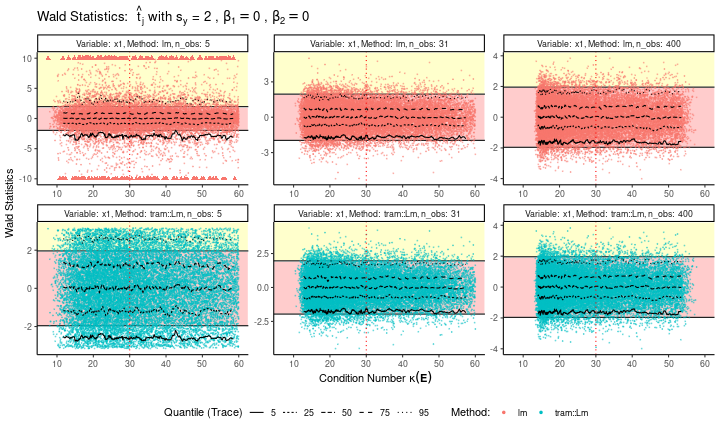
\includegraphics[width=0.85\textwidth]{../fromsim/simres_wald101-1.png}
\end{subfigure}
\begin{subfigure}[b]{1\textwidth}
\vspace*{-0.9cm}
\centering
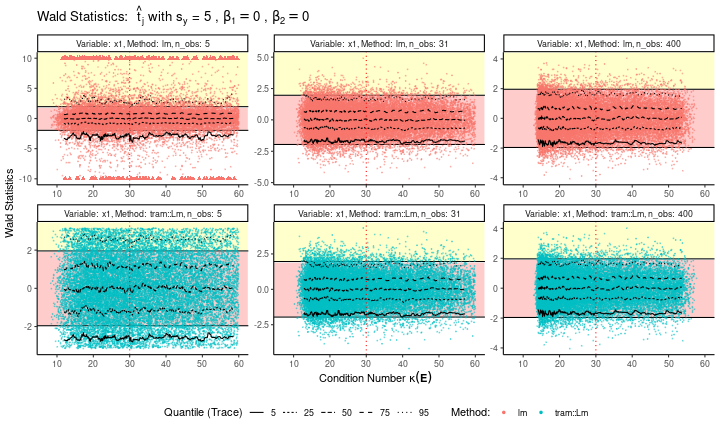
\includegraphics[width=0.85\textwidth]{../fromsim/simres_wald111-1.png}
\end{subfigure}
\begin{subfigure}[b]{1\textwidth}
\vspace*{-0.9cm}
\centering
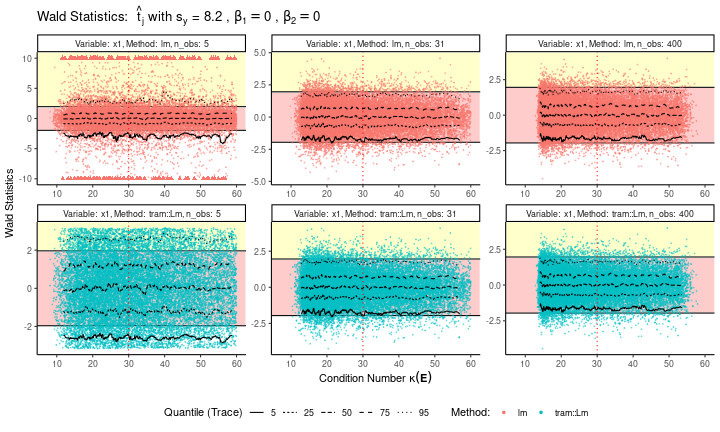
\includegraphics[width=0.85\textwidth]{../fromsim/simres_wald121-1.png}
\end{subfigure}
\vspace*{-1cm}
\caption{Wald statistics versus the condition number. The red shaded area represents Wald statistics between -1.96 and 1.96 which are non-detected signals and thus harmful. Points in the yellow shaded area are even more troublesome since they mean there is a detection, but the signal is incorrect. The frame of the plots are restricted to have maximum $y$-axis range between -10 and 10. Points laying outside are placed at the border and visualized as triangles.}
\label{fig:simres_wald2}
\end{figure}

%%%%%%%%%%%%%%%%%%%%%%%%%%%%%%%%%%%%%%%%%%%%%%%%%%%%%%%%%%%%%%%%%%%%%%%%%%%%%%%%
%\newpage
\vspace*{-1cm}
\subsection{Wald statistics difference vs. condition number: $\beta_1=-46.1$ and $\beta_2=-0.9$}
%%%%%%%%%%%%%%%%%%%%%%%%%%%%%%%%%%%%%%%%%%%%%%%%%%%%%%%%%%%%%%%%%%%%%%%%%%%%%%%%%
\begin{figure}[H]
\vspace*{-0.5cm}
\centering
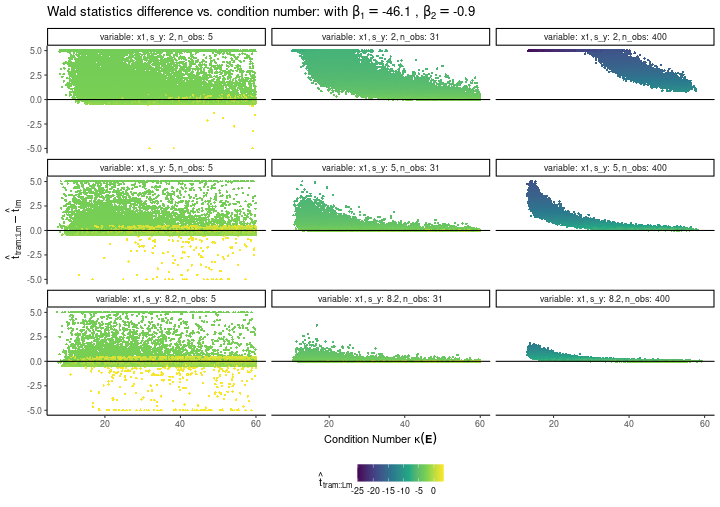
\includegraphics[width=0.85\textwidth]{../fromsim/simana11-1.png}
\vspace*{-0.5cm}
\caption{Wald statistics differences plotted versus the condition number and colored by the Wald statistics of the \texttt{tram::Lm} method. See description in Figure~\ref{fig:simres_differencevscondu2}.}
\label{fig:simres_differencevscondu1}
\end{figure}

%%%%%%%%%%%%%%%%%%%%%%%%%%%%%%%%%%%%%%%%%%%%%%%%%%%%%%%%%%%%%%%%%%%%%%%%%%%%%%%%
%\newpage
%\vspace*{-1cm}
\subsection{Wald statistics difference vs. condition number: $\beta_1=0$ and $\beta_2=0$}
%%%%%%%%%%%%%%%%%%%%%%%%%%%%%%%%%%%%%%%%%%%%%%%%%%%%%%%%%%%%%%%%%%%%%%%%%%%%%%%%%
\begin{figure}[H]
\centering
\vspace*{-0.5cm}
\centering
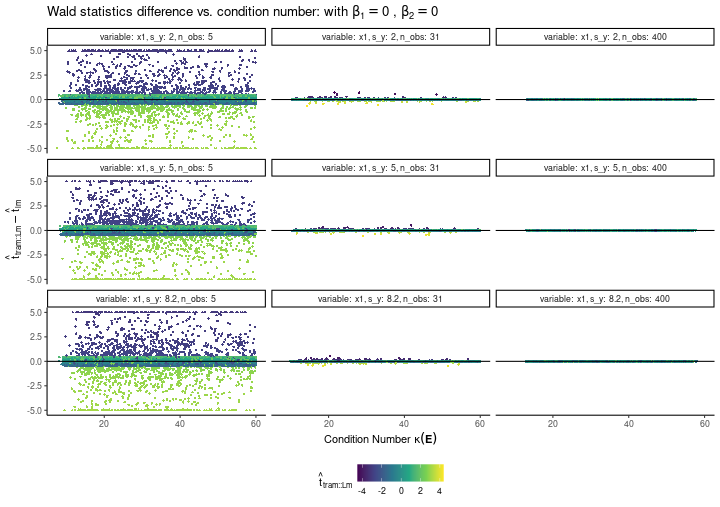
\includegraphics[width=0.85\textwidth]{../fromsim/simana41-1.png}
\vspace*{-0.5cm}
\caption{Wald statistics differences plotted versus the condition number and colored by the Wald statistics of the \texttt{tram::Lm} method. It seems like that the difference between the Wald statistics values decreases with increasing condition number and increasing noise \texttt{s\_y}. In addition, with higher sample sizes, the difference seems to be much more stable.}
\label{fig:simres_differencevscondu2}
\end{figure}


%%%%%%%%%%%%%%%%%%%%%%%%%%%%%%%%%%%%%%%%%%%%%%%%%%%%%%%%%%%%%%%%%%%%%%%%%%%%%%%%
%\newpage
\vspace*{-1cm}
\subsection{Proportion of significant results: $\beta_1=-46.1$ and $\beta_2=-0.9$}
%%%%%%%%%%%%%%%%%%%%%%%%%%%%%%%%%%%%%%%%%%%%%%%%%%%%%%%%%%%%%%%%%%%%%%%%%%%%%%%%%
\begin{figure}[H]
\begin{subfigure}[b]{1\textwidth}
\vspace*{-0.5cm}
\centering
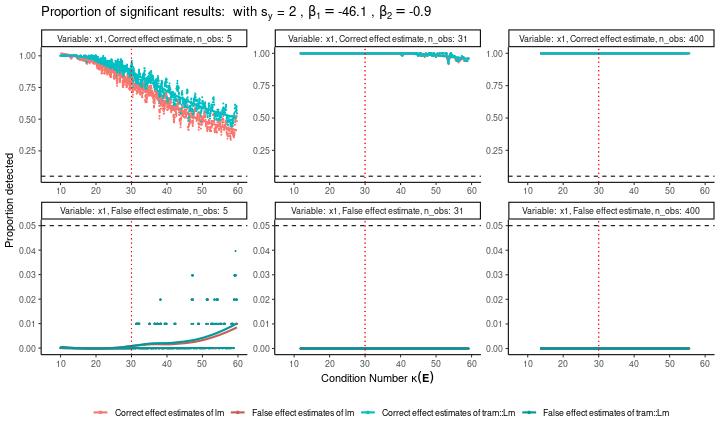
\includegraphics[width=0.85\textwidth]{../fromsim/simres_prop11-1.png}
\end{subfigure}
\begin{subfigure}[b]{1\textwidth}
\vspace*{-0.9cm}
\centering
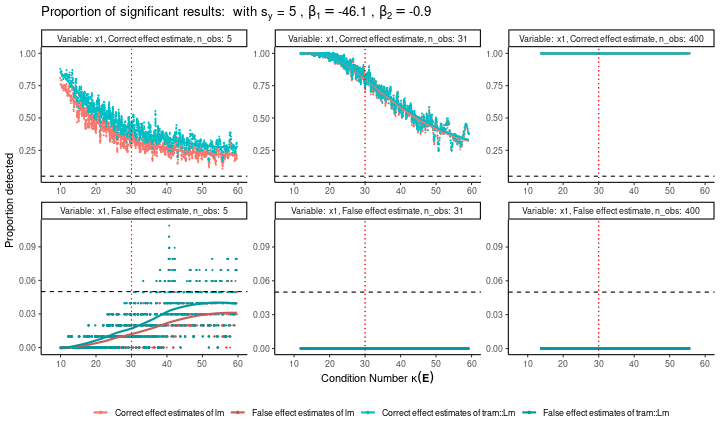
\includegraphics[width=0.85\textwidth]{../fromsim/simres_prop21-1.png}
\end{subfigure}
\begin{subfigure}[b]{1\textwidth}
\vspace*{-0.9cm}
\centering
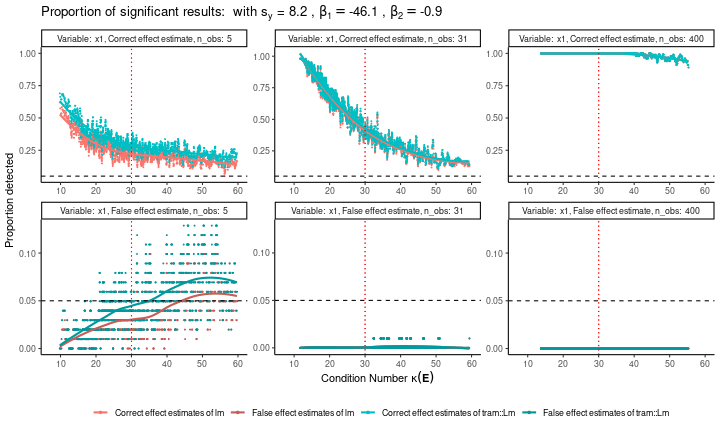
\includegraphics[width=0.85\textwidth]{../fromsim/simres_prop31-1.png}
\end{subfigure}
\vspace*{-0.9cm}
\caption{Obtained proportion of Wald statistics with correctly detected effect estimates ($\hat{t}_{ij}\leq -1.96$) and incorrectly detected effect estimates ($\hat{t}_{ij}\geq 1.96$). The proportions are calculated similarly to the moving quantile procedure: We gather 100 observations, calculate the proportions and the location thereof determined by the median condition number. Then the window moves forward by discarding 10 observations but adding the next 10 and computes the proportion and location again. This procedure is then done until the end of the frame.}
\label{fig:simres_prop1}
\end{figure}

%%%%%%%%%%%%%%%%%%%%%%%%%%%%%%%%%%%%%%%%%%%%%%%%%%%%%%%%%%%%%%%%%%%%%%%%%%%%%%%%
%\newpage
\vspace*{-1cm}
\subsection{Proportion of significant results: $\beta_1=0$ and $\beta_2=0$}
%%%%%%%%%%%%%%%%%%%%%%%%%%%%%%%%%%%%%%%%%%%%%%%%%%%%%%%%%%%%%%%%%%%%%%%%%%%%%%%%%
\begin{figure}[H]
\begin{subfigure}[b]{1\textwidth}
\vspace*{-0.5cm}
\centering
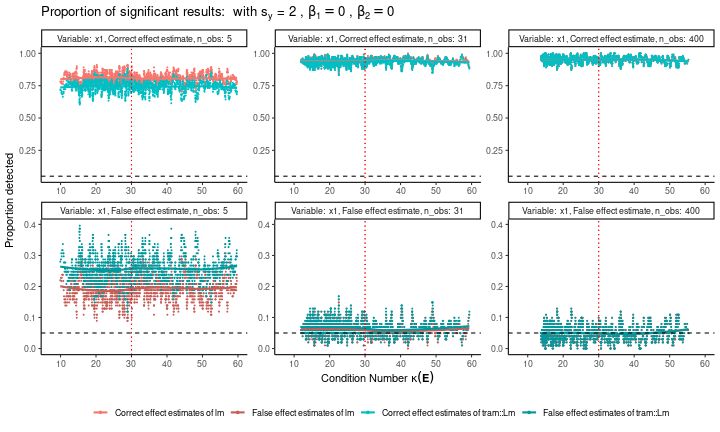
\includegraphics[width=0.85\textwidth]{../fromsim/simres_prop101-1.png}
\end{subfigure}
\begin{subfigure}[b]{1\textwidth}
\vspace*{-0.9cm}
\centering
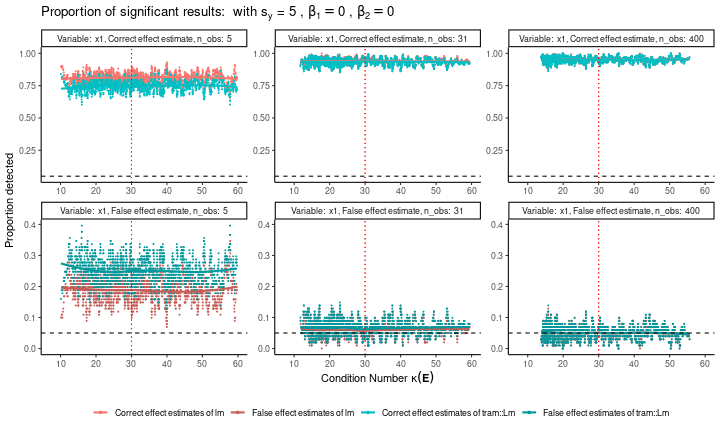
\includegraphics[width=0.85\textwidth]{../fromsim/simres_prop111-1.png}
\end{subfigure}
\begin{subfigure}[b]{1\textwidth}
\vspace*{-0.9cm}
\centering
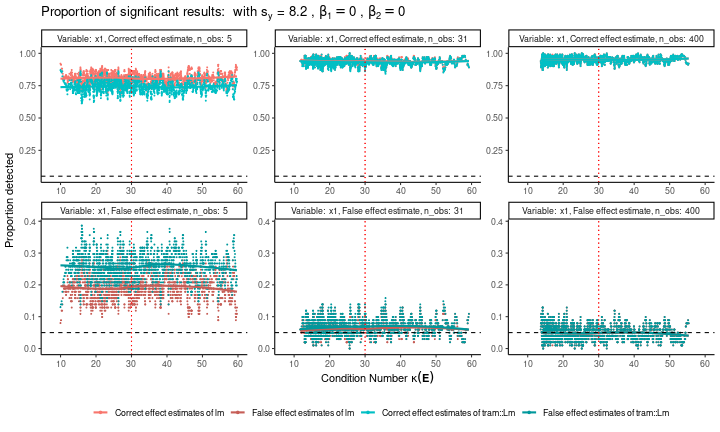
\includegraphics[width=0.85\textwidth]{../fromsim/simres_prop121-1.png}
\end{subfigure}
\vspace*{-0.9cm}
\caption{Obtained proportion of Wald statistics with correctly detected effect estimates ($\hat{t}_{ij}\leq -1.96$) and incorrectly detected effect estimates ($\hat{t}_{ij}\geq 1.96$). In the situation where $\beta_j=0$, correct means a non-significant result ($-1.96<\hat{t}_{ij}< 1.96$). The proportions are calculated similarly to the moving quantile procedure: We gather 100 observations, calculate the proportions and the location thereof determined by the median condition number. Then the window moves forward by discarding 10 observations but adding the next 10 and computes the proportion and location again. }
\label{fig:simres_prop2}
\end{figure}

%%%%%%%%%%%%%%%%%%%%%%%%%%%%%%%%%%%%%%%%%%%%%%%%%%%%%%%%%%%%%%%%%%%%%%%%%%%%%%%%
%\newpage
\vspace*{-1cm}
\subsection{Wald statistics ratio: $\beta_1=-46.1$ and $\beta_2=-0.9$}\label{sec:compwald1}
%%%%%%%%%%%%%%%%%%%%%%%%%%%%%%%%%%%%%%%%%%%%%%%%%%%%%%%%%%%%%%%%%%%%%%%%%%%%%%%%%
\begin{figure}[H]
\vspace*{-0.5cm}
\centering
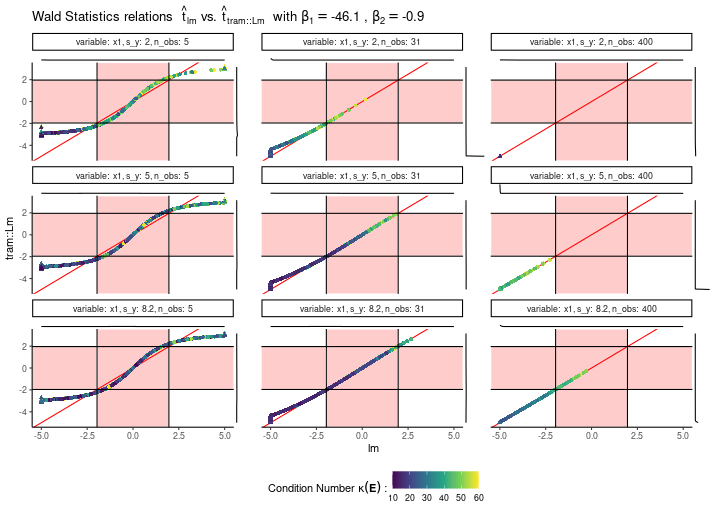
\includegraphics[width=0.85\textwidth]{../fromsim/simres_bivar11-1.png}
\vspace*{-0.5cm}
\caption{Direct comparison of Wald statistics. See description in Figure~\ref{fig:simres_bivar2}.}
\label{fig:simres_bivar1}
\end{figure}

%%%%%%%%%%%%%%%%%%%%%%%%%%%%%%%%%%%%%%%%%%%%%%%%%%%%%%%%%%%%%%%%%%%%%%%%%%%%%%%%
%\newpage
%\vspace*{-1cm}
\subsection{Wald statistics ratio: $\beta_1=0$ and $\beta_2=0$}
%%%%%%%%%%%%%%%%%%%%%%%%%%%%%%%%%%%%%%%%%%%%%%%%%%%%%%%%%%%%%%%%%%%%%%%%%%%%%%%%%
\begin{figure}[H]
\centering
\vspace*{-0.5cm}
\centering
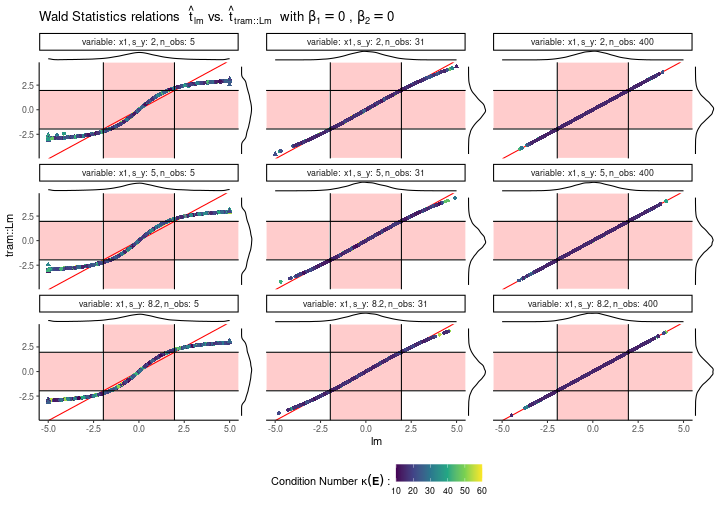
\includegraphics[width=0.85\textwidth]{../fromsim/simres_bivar41-1.png}
\vspace*{-0.5cm}
\caption{Direct comparison of Wald statistics resulting from the two different methods. Due to the paired design we can directly compare the two Wald statistics and if they are the very same, the points lay on the red diagonal. To have an impression about the distribution of the points, marginal densities are added at the sides. In general, it seems like that \texttt{lm} has larger Wald statistics than \texttt{tram::Lm} especially when $\hat{t}_\texttt{lm}$ is large. On the other hand, if  $\hat{t}_\texttt{lm}$ is low, $\hat{t}_\texttt{tram::Lm}$ tends to be larger in magnitude.}
\label{fig:simres_bivar2}
\end{figure}

%%%%%%%%%%%%%%%%%%%%%%%%%%%%%%%%%%%%%%%%%%%%%%%%%%%%%%%%%%%%%%%%%%%%%%%%%%%%%%%%
%\newpage
\vspace*{-1cm}
\subsection{Wald statistics difference vs. Wald statistics of \texttt{lm}: $\beta_1=-46.1$ and $\beta_2=-0.9$}
%%%%%%%%%%%%%%%%%%%%%%%%%%%%%%%%%%%%%%%%%%%%%%%%%%%%%%%%%%%%%%%%%%%%%%%%%%%%%%%%%
\begin{figure}[H]
\begin{subfigure}[b]{1\textwidth}
\vspace*{-0.5cm}
\centering
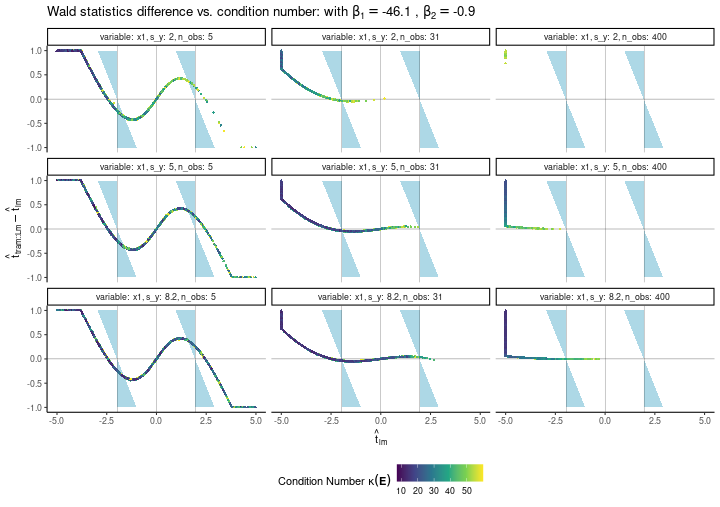
\includegraphics[width=0.95\textwidth]{../fromsim/simdiffvswald111-1.png}
\end{subfigure}
\begin{subfigure}[b]{1\textwidth}
\vspace*{-0.3cm}
\centering
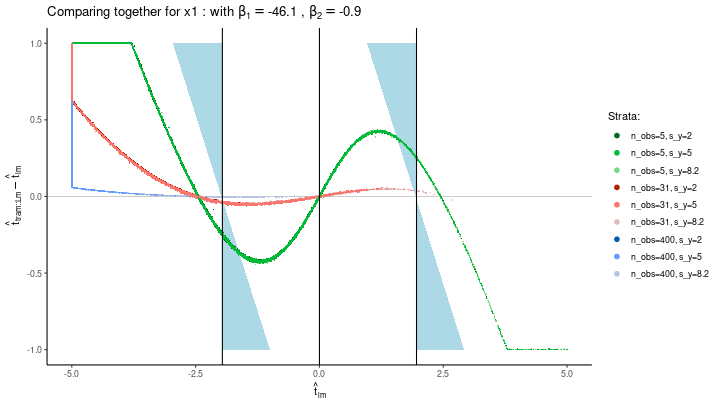
\includegraphics[width=0.95\textwidth]{../fromsim/simdiffvswald112-1.png}
\end{subfigure}
\vspace*{-0.9cm}
\caption{Wald statistics differences plotted versus the Wald statistics of the \texttt{lm} method and colored by the condition number in the upper plot. Comparison of all panels in the lower plot, but now colored with respect to the panels. The light blue area represents the area where \texttt{lm} and \texttt{tram::Lm} yield Wald statistics values that are interpreted differently in terms of significance for the generally used type 1 error rate of $\alpha$=0.05 ($f(\hat{t}_\text{lm})=\text{sign}(\hat{t}_\text{lm})\cdot q_{1-\alpha/2,Z} -\hat{t}_\text{lm}$). It seems to be the case that \texttt{tram::Lm} yields Wald statistics values that are more frequently interpretable as significant, independent of the direction. This effect seems to vanish with increasing sample size. The lower plot shows that the curves do not differ too much with the noise of the data (\texttt{s\_y}). However, the upper plot reveals that the condition number is then different and therefore hints towards the fact that the same Wald statistics can be obtained by different combinations of, here, \texttt{s\_y} and $\kappa\left(\bE\right)$ values. }
\label{fig:simres_differencevslm1}
\end{figure}

%%%%%%%%%%%%%%%%%%%%%%%%%%%%%%%%%%%%%%%%%%%%%%%%%%%%%%%%%%%%%%%%%%%%%%%%%%%%%%%%
%\newpage
\vspace*{-1cm}
\subsection{Wald statistics difference vs. Wald statistics of \texttt{lm}: $\beta_1=0$ and $\beta_2=0$}
%%%%%%%%%%%%%%%%%%%%%%%%%%%%%%%%%%%%%%%%%%%%%%%%%%%%%%%%%%%%%%%%%%%%%%%%%%%%%%%%%
\begin{figure}[H]
\begin{subfigure}[b]{1\textwidth}
\vspace*{-0.5cm}
\centering
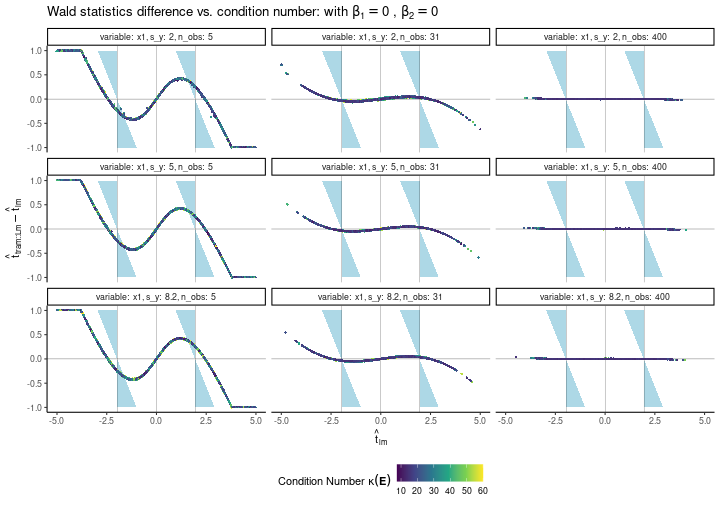
\includegraphics[width=0.95\textwidth]{../fromsim/simdiffvswald411-1.png}
\end{subfigure}
\begin{subfigure}[b]{1\textwidth}
\vspace*{-0.3cm}
\centering
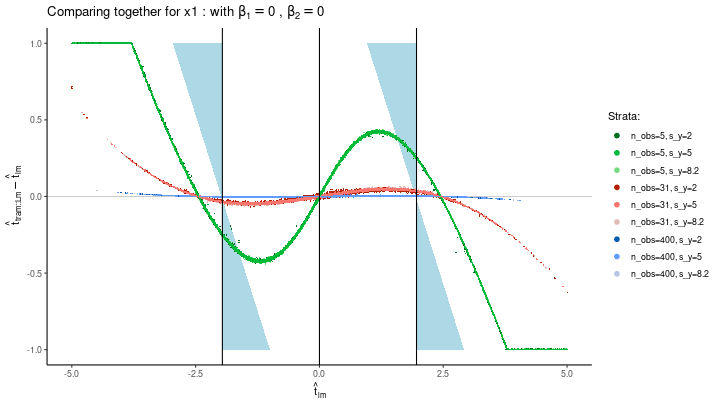
\includegraphics[width=0.95\textwidth]{../fromsim/simdiffvswald412-1.png}
\end{subfigure}
\vspace*{-0.9cm}
\caption{Wald statistics differences plotted versus the Wald statistics of the \texttt{lm} method and colored by the condition number in the upper plot. Comparison of all panels in the lower plot, but now colored with respect to the panels. The light blue area represents the area where \texttt{lm} and \texttt{tram::Lm} yield Wald statistics values that are interpreted differently in terms of significance for the generally used type 1 error rate of $\alpha$=0.05 ($f(\hat{t}_\text{lm})=\text{sign}(\hat{t}_\text{lm})\cdot q_{1-\alpha/2,Z} -\hat{t}_\text{lm}$). It seems to be the case that \texttt{tram::Lm} yields Wald statistics values that are more frequently interpretable as significant, independent of the direction. This effect seems to vanish with increasing sample size. The lower plot shows that the curves do not differ too much with the noise of the data (\texttt{s\_y}). However, the upper plot reveals that the condition number is then different and therefore hints towards the fact that the same Wald statistics can be obtained by different combinations of, here, \texttt{s\_y} and $\kappa\left(\bE\right)$ values. }
\label{fig:simres_differencevslm2}
\end{figure}


%%%%%%%%%%%%%%%%%%%%%%%%%%%%%%%%%%%%%%%%%%%%%%%%%%%%%%%%%%%%%%%%%%%%%%%%%%%%%%%%
\newpage
\section{Sample size correction}
%%%%%%%%%%%%%%%%%%%%%%%%%%%%%%%%%%%%%%%%%%%%%%%%%%%%%%%%%%%%%%%%%%%%%%%%%%%%%%%%
Figure~\ref{fig:simres_nrel1} and \ref{fig:simres_nrel2} show the relative number of observations (sample size needed divided by the current sample size) that is needed to reach the power of 80\% with the current collinearity magnitude. The needed sample size is determined by the function \texttt{Collinearity::copowerlm} and works so far only for the \texttt{lm} method. The relevant effect estimate for $\beta_1$ that we want to find, given it is there, is $\beta_1=-46.1$ and is in both figures the same, leading to very similar dynamics. We see that with increasing collinearity and increasing noise in the form of large \texttt{s\_y}, the needed sample size gets larger. Furthermore, the lower the current sample size, the more variability in the predicted sample size needed.

%%%%%%%%%%%%%%%%%%%%%%%%%%%%%%%%%%%%%%%%%%%%%%%%%%%%%%%%%%%%%%%%%%%%%%%%%%%%%%%%
%\vspace*{-1cm}
\newpage
\subsection{Study design - Relative sample size needed: $\beta_1=-46.1$ and $\beta_2=-0.9$}
%%%%%%%%%%%%%%%%%%%%%%%%%%%%%%%%%%%%%%%%%%%%%%%%%%%%%%%%%%%%%%%%%%%%%%%%%%%%%%%%%
\begin{figure}[H]
\centering
\begin{subfigure}[b]{1\textwidth}
\vspace*{-0.5cm}
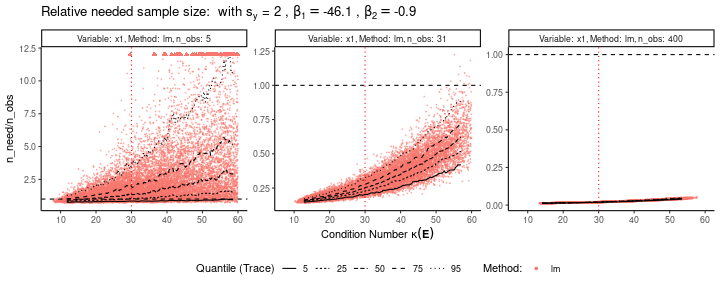
\includegraphics[width=1\textwidth]{../fromsim/simres_nrel1-1.png}
\end{subfigure}
\begin{subfigure}[b]{1\textwidth}
\vspace*{-1cm}
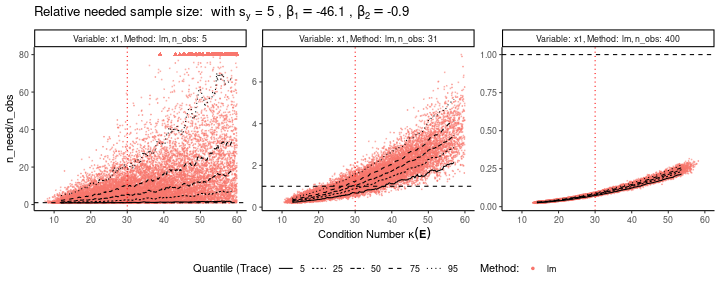
\includegraphics[width=1\textwidth]{../fromsim/simres_nrel2-1.png}
\end{subfigure}
\begin{subfigure}[b]{1\textwidth}
\vspace*{-1cm}
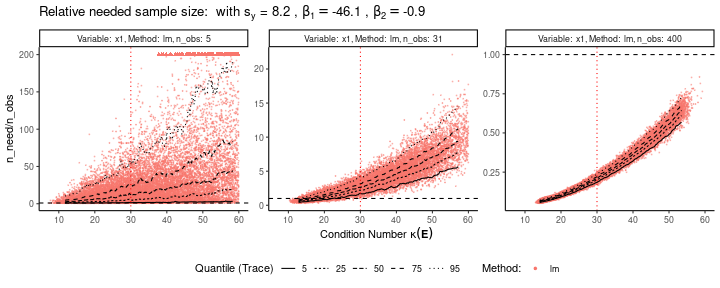
\includegraphics[width=1\textwidth]{../fromsim/simres_nrel3-1.png}
\end{subfigure}
\caption{Number of observations needed to reach the power of 80\% with the given collinearity magnitude expressed by the condition number. It gets visible that the condition number does not uniquely define the collinearity within $\X$ as no straight line is plotted. Further, we see that with higher condition number, but also with higher \texttt{s\_y}, the needed sample size increases. We also note, that with very low sample sizes, the uncertainty of predicted needed sample size gets very large.}
\label{fig:simres_nrel1}
\end{figure}
%%%%%%%%%%%%%%%%%%%%%%%%%%%%%%%%%%%%%%%%%%%%%%%%%%%%%%%%%%%%%%%%%%%%%%%%%%%%%%%%
\newpage
\vspace*{-1cm}
\subsection{Study design - Relative sample size needed: $\beta_1=0$ and $\beta_2=0$}
%%%%%%%%%%%%%%%%%%%%%%%%%%%%%%%%%%%%%%%%%%%%%%%%%%%%%%%%%%%%%%%%%%%%%%%%%%%%%%%%%
\begin{figure}[H]
\centering
\begin{subfigure}[b]{1\textwidth}
\vspace*{-0.5cm}
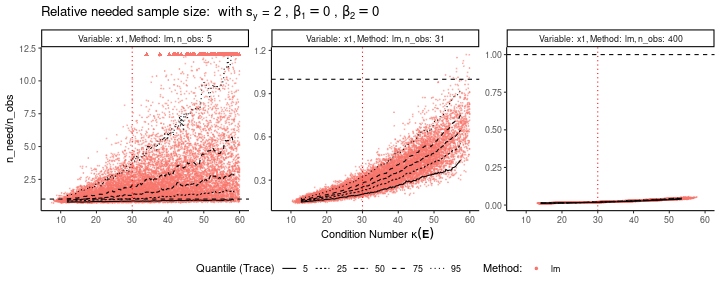
\includegraphics[width=1\textwidth]{../fromsim/simres_nrel10-1.png}
\end{subfigure}
\begin{subfigure}[b]{1\textwidth}
\vspace*{-1cm}
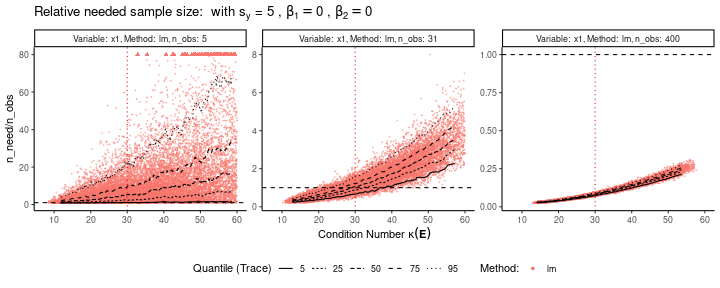
\includegraphics[width=1\textwidth]{../fromsim/simres_nrel11-1.png}
\end{subfigure}
\begin{subfigure}[b]{1\textwidth}
\vspace*{-1cm}
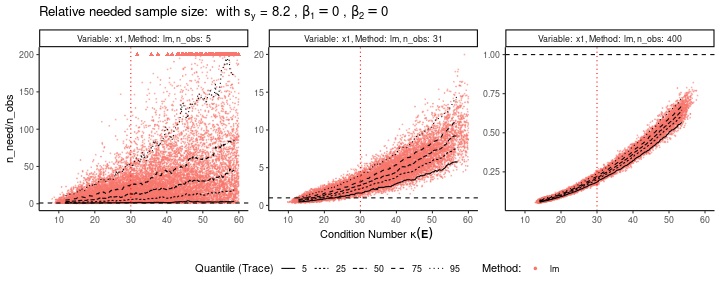
\includegraphics[width=1\textwidth]{../fromsim/simres_nrel12-1.png}
\end{subfigure}
\caption{Number of observations needed to reach the power of 80\% with the given collinearity magnitude expressed by the condition number. It gets visible that the condition number does not uniquely define the collinearity within $\X$ as no straight line is plotted. Further, we see that with higher condition number, but also with higher \texttt{s\_y}, the needed sample size increases. We also note, that with very low sample sizes, the uncertainty of predicted needed sample size gets very large. The results are very much the same as in Figure~\ref{fig:simres_nrel1} since the effect the sample size calculation is based on, is the same and does not matter if it is actually there or not.}
\label{fig:simres_nrel2}
\end{figure}







%%%%%%%%%%%%%%%%%%%%%%%%%%%%%%%%%%%%%%%%%%%%%%%%%%%%%%%%%%%%%%%%%%%%%%


% LaTeX file for Chapter 07



%%%%%%%%%%%%%%%%%%%%%%%%%%%%%%%%%%%%
\chapter{Results: Collinearity fingerprint and graph}\label{chap:collfinger}
%%%%%%%%%%%%%%%%%%%%%%%%%%%%%%%%%%%%



We are approaching the end of this master thesis and have now more knowledge about the troubles that come with collinearity.
Therefore, let us revise on the paper of \cite{Harrison1978} introduced in Chapter~\ref{chap:boston_intro}. It seems that they have arrived at their goal to investigate the willingness to pay for clean air. They found a one unit increase in $\texttt{nox}^2$ (\texttt{nox}: Nitrogen oxide concentration in pphm) leads to an increase in $\log\left(\text{Median value of owner-occupied homes in USD}\right)$ of -0.0064 with 95\% confidence interval of (-0.0086, -0.0042).
Since the confidence interval does not include zero, the result is said to be statistically significant on the 95\% confidence level.

Now time has passed since 1978 and maybe someone wants to reproduce the results or want to conduct a similar study in a different area. A natural question that arises is the number of observations that are needed to show the effect given it is there. The number of observations in \cite{Harrison1978} is $n=506$ and each point belongs to a certain census tract in the Boston Standard Metropolitan Statistical Area (SMSA) in 1970. $n=506$ was enough for the researchers to make their point in terms of having statistically significant results. But what if one is interested in an area that does not have that many observations or has to be gathered first?

Thus, a sample size calculation is needed. And we think there are two good reasons for this, independent of the type of research:
\begin{enumerate}
\item If data is already available: Determine whether a null-finding is likely due to the fact that the effect is not there or the sample size was too low to show it.
\item If data has to be gathered: Have an idea about the amount of resources that need to be invested to get the data.
\end{enumerate}
Hopefully, this convinces the reader that a sample size calculation is in both cases of use.
% ##################################
\section{Sample size calculation}
% ##################################

% ====================================
\subsection{Parametrization of Harrison and Rubinfeld}
% ====================================



\begin{program}[h]
\begin{knitrout}
\definecolor{shadecolor}{rgb}{0.969, 0.969, 0.969}\color{fgcolor}\begin{kframe}
\begin{alltt}
\hlcom{# Sample size calculation}
\hlstd{n_boston} \hlkwb{<-} \hlstd{Collinearity}\hlopt{::}\hlkwd{copowerlm}\hlstd{(}\hlkwc{power} \hlstd{=} \hlnum{0.8}\hlstd{,} \hlkwc{alpha} \hlstd{=} \hlnum{0.05}\hlstd{,}
               \hlkwc{Delta} \hlstd{= Delta,}
               \hlkwc{sigma} \hlstd{=} \hlkwd{sigma}\hlstd{(mpaper),} \hlkwc{p}\hlstd{=} \hlkwd{nrow}\hlstd{(trouble) ,}
               \hlkwc{voilen} \hlstd{=} \hlkwd{var}\hlstd{(BostonHousing2}\hlopt{$}\hlstd{nox}\hlopt{^}\hlnum{2}\hlstd{)}\hlopt{+}\hlkwd{mean}\hlstd{(BostonHousing2}\hlopt{$}\hlstd{nox}\hlopt{^}\hlnum{2}\hlstd{)}\hlopt{^}\hlnum{2}\hlstd{,}
               \hlkwc{trouble} \hlstd{=} \hlkwd{diag}\hlstd{(trouble)[}\hlstr{"I(nox^2)"}\hlstd{] )}
\hlstd{n_boston} \hlkwb{<-} \hlkwd{ceiling}\hlstd{(n_boston}\hlopt{$}\hlstd{n)}
\end{alltt}
\end{kframe}
\end{knitrout}
\caption{Application of the \texttt{copowerlm} function. \texttt{mpaper} is the so-called basic equation model fitted in \cite{Harrison1978}. The effects we want the test to be powered for is the effect we found with the model and the corresponding 95\% confidence interval boundaries as
$\texttt{Delta}=\texttt{c}\left(-0.0085648, -0.0063724, -0.00418\right)$. The part that introduces collinearity is \texttt{trouble}=$\text{diag}\left(\left(\bE^\top\bE\right)^{-1}\right)[\texttt{"I(nox\textasciicircum 2")}]$ where $\bE$ is the equilibrated design matrix extracted from the model.}
\label{code:nboston}
\end{program}

Let us have a first look at how many observations \cite{Harrison1978} really would have needed to show the same effect with a common power of 80\%. Since we are no expert in this field of study, a determination of a relevant effect size from our side may be quite arbitrary. Thus, we will do the sample size calculation for 3 different effect sizes, namely the effect estimate and the lower and upper bound of the corresponding 95\% confidence interval (computed in Table~\ref{tab:reg_bo}).

Thus, we apply \texttt{copowerlm} as is visible in \textsf{R}-Code~\ref{code:nboston} and from this calculation we get $n=\texttt{c}\left(70, 124, 285\right)$. Since we know the underlying effect size of the model, we can verify the sample size calculation by repeated sampling of $n=124$ observations without replacement and subsequent model fitting.



\begin{figure}[h!]%H is strict!
\begin{center}
\begin{knitrout}
\definecolor{shadecolor}{rgb}{0.969, 0.969, 0.969}\color{fgcolor}
\includegraphics[width=\maxwidth]{figure/ch07_figwald_sig_plot-1} 
\end{knitrout}
\end{center}
\vspace*{-0.7cm}
\caption{Wald statistics dynamic for $B=200$ repeated draws of size $n=124$ from the whole \texttt{BostonHousing2} data set to verify the sample size calculation. The empirically determined power for variable $\texttt{nox}^2$ is 0.8 for the \texttt{lm} model and 0.845 for the \texttt{tram::Lm} model.}
\label{fig:wald_sig_plot}
\end{figure}

Figure~\ref{fig:wald_sig_plot} shows the Wald statistics of the repeatedly drawn data sets plotted against the calculated condition number for both methods. The empirically determined power for variable $\texttt{nox}^2$ is for the \texttt{lm} model 0.8 which is quite close to the initially wanted power of 0.80. The power for the \texttt{tram::Lm} model is with 0.845 slightly higher than in the \texttt{lm} case. Although the sample size calculation is based on the least-squares approach and parametrization, it seems to be the case that the results from \texttt{tram::Lm} behave for this particular example similarly to the results of \texttt{lm}.

% \begin{figure}[h!]%H is strict!
% \begin{center}

% \end{center}
% \caption{Wald statistics dynamic for $B=B$ repeated draws of size $n=n_boston[2]$ from the whole \texttt{BostonHousing2} data set for the variables that are not of primary interest.}
% \label{fig:ws_ni_plot}
% \end{figure}

% ====================================
\subsection{Non-transformed parametrization}
% ====================================



We also do the same sample size calculation for the non-transformed parametrization. We want to have the model powered for the same relevant effect size, and thus we take \texttt{Delta=c}(-1942.524, -1571.469, -1120.881) which corresponds to the translated estimate from the \texttt{mpaper} model as already described in Section~\ref{sec:basiceqboston}.



\begin{program}[h]
\begin{knitrout}
\definecolor{shadecolor}{rgb}{0.969, 0.969, 0.969}\color{fgcolor}\begin{kframe}
\begin{alltt}
\hlcom{# Sample size calculation}
\hlstd{n_simpler} \hlkwb{<-} \hlstd{Collinearity}\hlopt{::}\hlkwd{copowerlm}\hlstd{(}\hlkwc{power} \hlstd{=} \hlnum{0.8}\hlstd{,} \hlkwc{alpha} \hlstd{=} \hlnum{0.05}\hlstd{,}
                     \hlkwc{Delta} \hlstd{= Delta,}
                     \hlkwc{sigma} \hlstd{=} \hlkwd{sigma}\hlstd{(msimpler),} \hlkwc{p}\hlstd{=} \hlkwd{nrow}\hlstd{(troublesimpler) ,}
                     \hlkwc{voilen} \hlstd{=} \hlkwd{var}\hlstd{(BostonHousing2}\hlopt{$}\hlstd{nox)}\hlopt{+}\hlkwd{mean}\hlstd{(BostonHousing2}\hlopt{$}\hlstd{nox)}\hlopt{^}\hlnum{2}\hlstd{,}
                     \hlkwc{trouble} \hlstd{=} \hlkwd{diag}\hlstd{(troublesimpler)[}\hlstr{"nox"}\hlstd{] )}
\hlstd{n_simpler} \hlkwb{<-} \hlkwd{ceiling}\hlstd{(n_simpler}\hlopt{$}\hlstd{n)}
\end{alltt}
\end{kframe}
\end{knitrout}
\caption{Application of the \texttt{copowerlm} function. \texttt{msimpler} is the simpler model fitted without any transformation of the variables. The effects we want the test to be powered for is the effect and the corresponding 95\% confidence interval boundaries determined by the model fitted in \cite{Harrison1978} but translated on the original housing value scale (\ref{sec:basiceqboston}). Thus, $\texttt{Delta}=\texttt{c}\left(-1942.524, -1571.469, -1120.881\right)$. The part that introduces collinearity is \texttt{trouble}=$\text{diag}\left(\left(\bE^\top\bE\right)^{-1}\right)[\texttt{"I(nox\textasciicircum 2")}]$ where $\bE$ is the equilibrated design matrix extracted from the model.}\label{code:nsimpler}
\end{program}

\textsf{R}-Code~\ref{code:nsimpler} shows the computation which results in sample sizes of $n=\texttt{c}$(153, 233, 455) and thus we note that with this model we need a considerable amount more data to arrive at the same power.

% ##################################
\section{Collinearity fingerprint with bootstrap}
% ##################################

We have seen that collinearity can lead to unstable effect estimates. This usually results in a non-detection as the standard error of the effect estimate overwhelms the signal. But there are situations, especially when the sample size is low, where this is not the case and signals are proportionally high and result in a large Wald statistics. Due to the instability, these signals can point into the wrong direction, which is very dangerous in terms of making a decision. Thus, it is crucial to invest the reliability of the estimation process when high collinearity is present, especially when accompanied by low sample sizes.

Investigating the reliability can be checked for instance with bootstrapping \citep{Efron1986} as it is also done for example in selecting variables \citep{Altman1989,Heinze2018}.
This idea is implemented in the function \texttt{Collinearity::cofingerprint}.
In our situation this means that for one bootstrap sample we draw from the \texttt{BostonHousing2} data set 506 observations with replacement. Then, for each of these data sets, the model is again fitted. Plotting this procedure on the scale of the Wald statistics shows whether significant results can be trusted or not. Figure~\ref{fig:coll_boot1} shows the results for the parametrization that is used in the paper for the least-squares and transformation model, and Figure~\ref{fig:coll_boot2} shows the same for the non-transformed model. Although as mentioned in Section~\ref{sec:mltramLM} the design matrix and therefore also the variance decomposition is not exactly defined, the investigation of the collinearity fingerprint is applied on the part of the model that is returned by the command \texttt{model.matrix()}. For the \texttt{lm} case this means that the intercept is also investigated, but for the \texttt{tram::Lm} model only the explanatory variables without transformation function parts are provided.

\begin{program}[H]
\begin{knitrout}
\definecolor{shadecolor}{rgb}{0.969, 0.969, 0.969}\color{fgcolor}\begin{kframe}
\begin{alltt}
\hlcom{# Collinearity fingerprint with bootstrap}
\hlstd{Collinearity}\hlopt{::}\hlkwd{cofingerprint}\hlstd{(mpaper,}
        \hlkwc{B} \hlstd{= B,}
        \hlkwc{ncon} \hlstd{= ncon,} \hlcom{# Number of printed condition indices}
        \hlkwc{main} \hlstd{=} \hlstr{"Collinearity Fingerprint - Least Squares (lm)"}\hlstd{,}
        \hlkwc{alpha} \hlstd{=} \hlnum{0.05}\hlstd{,}
        \hlkwc{cex.vd} \hlstd{=} \hlnum{1.4}\hlstd{,} \hlkwc{cex.main} \hlstd{=} \hlnum{1.5}\hlstd{,} \hlkwc{cex.prop}  \hlstd{=} \hlnum{0.9}\hlstd{,} \hlkwc{ydi} \hlstd{=} \hlnum{10}
        \hlstd{)}
\end{alltt}
\end{kframe}
\end{knitrout}
\caption{Application of the \texttt{cofingerprint} function. \texttt{mpaper} is the so called basic equation model fitted in \cite{Harrison1978}. The source code of the function \texttt{cofingerprint} can be found in the \texttt{Collinearity} package.}\label{code:collfingerprint}
\end{program}

\newpage
\begin{figure}[H]%H is strict!
\centering
\begin{knitrout}
\definecolor{shadecolor}{rgb}{0.969, 0.969, 0.969}\color{fgcolor}
\includegraphics[width=\maxwidth]{figure/ch07_figcoll_boot11-1} 

\includegraphics[width=\maxwidth]{figure/ch07_figcoll_boot11-2} 
\end{knitrout}
\vspace*{-10mm}
\caption{Wald statistics dynamic for $B=500$ repeated draws of size $n=506$ with replacement from the whole \texttt{BostonHousing2} data set with the model used in \cite{Harrison1978}. Underneath the title of the plot are the condition indices printed determined with the \texttt{Collinearity} package, and the 3 largest thereof are also visualized within the plot.
The variance proportions are also added with the strength of color corresponding to their size, meaning that lower proportions are more likely to be transparent. In addition, the proportion of $t$ values that are considered as significant on the 5\% significance level is printed as well for each variable.}
\label{fig:coll_boot1}
\end{figure}

\newpage
\begin{figure}[H]%H is strict!
\begin{center}
\begin{knitrout}
\definecolor{shadecolor}{rgb}{0.969, 0.969, 0.969}\color{fgcolor}
\includegraphics[width=\maxwidth]{figure/ch07_figcoll_boot2-1} 

\includegraphics[width=\maxwidth]{figure/ch07_figcoll_boot2-2} 
\end{knitrout}
\end{center}
\vspace*{-10mm}
\caption{Wald statistics dynamic for $B=500$ repeated draws of size $n=506$ with replacement from the whole \texttt{BostonHousing2} data set with the simpler model using all variables non-transformed. Underneath the title of the plot are the condition indices printed determined with the \texttt{Collinearity} package, and the 2 largest thereof are also visualized within the plot.
The variance proportions are also added with the strength of color corresponding to their size, meaning that lower proportions are more likely to be transparent. In addition, the proportion of $t$ values that are considered as significant on the 5\% significance level is printed as well for each variable.}
\label{fig:coll_boot2}
\end{figure}


% ##################################
\section{Collinearity zoom-in: Who is responsible?}
% ##################################

Equation~\eqref{eq:squaredwaldpart} points out four key components why a signal can go undetected, and the part that relates to collinearity is the $\bR_\X^2$ term, which describes how well the variable of interest can be explained by a linear combination of the other remaining variables (\ref{sec:rsquared}). However, the $\bR_\X^2$ is a single value and does not tell which variable specifically explains the variable of interest well and is therefore responsible for the potentially inconvenient results. Thus, to investigate this issue further, we visualize the relation of the variable of interest to all the other explanatory variables by a multiple linear regression model.
Figure~\ref{fig:dag} illustrates this concept that is integrated in the \texttt{Collinearity::cotograph} function.
The $\bR_\X^2$ value is plotted in the central node that corresponds to the variable of interest (\texttt{voi}).
Variables that have a high Wald statistics ($t$) have high explanatory power of the variable of interest and should be closely inspected.

Still, this diagnostics is also susceptible to collinearity, which means that a high $\bR_\X^2$ can appear even without high individual Wald statistics, since collinearity within this model also leads to the effect to go undetected. 
Thus, we can say that variables associated with high $t$ will contribute to  high $\bR_\X^2$, but it does not necessarily detect all variables.
The \texttt{cotograph} function has an argument, \texttt{subR2}, which by default is set to \texttt{FALSE}, but can be changed to \texttt{TRUE} to understand the underlying collinearity not directly related to the variable of interest. With \texttt{subR2} set to \texttt{TRUE}, a separate multiple linear regression model is fitted for each explanatory variable, excluding the variable of interest (\texttt{voi}). The fits are then quantified by $\bR_\X^2$ and displayed in the nodes of the corresponding variable. Explanatory variables with high $\bR_\X^2$ values are affected by collinearity, meaning their effect on the variable of interest (\texttt{voi}) is weakened, expressed by a lower $t$.
% To get an idea about the underlying collinearity that does not directly relate to the variable of interest, \texttt{cotograph} has the argument \texttt{subR2} which is per default \texttt{FALSE} but can be turned to \texttt{TRUE}. By doing this, for each explanatory variable a separate multiple linear regression model is fitted containing all other explanatory variables apart from \texttt{voi}.
% All the fits are then also quantified by $\bR_\X^2$ and appear in the nodes of the corresponding variable.
% Explanatory variables that are accompanied by a large \texttt{subR2} are affected by collinearity, meaning that their effect on the variable of interest is attenuated expressed by a lower $t$.

All diagnostic measures in these plots are calculated with the least-squares method and the variables considered in the plot are the ones that appear when calling the command \texttt{model.matrix()} which provides for the \texttt{lm} model the explanatory variables including intercept if used. For the \texttt{tram::Lm} model, only the explanatory variables are returned, and we remind that the part corresponding to the transformation of the outcome may also contribute to collinearity but is not inspected in this case.
Furthermore, this diagnostic procedure does not necessarily have to agree with the Variance decomposition matrix suggested by Belsley in Tables~\ref{tab:vardecomp} and \ref{tab:vardecomp_tram}.
This, because Belsley's procedure quantifies the overall collinearity composition and does not target one specific variable of interest, as it is done in the \texttt{Collinearity::cotograph} function.
Thus, \texttt{cotograph} provides more an alternative to the Variance decomposition matrix.

\begin{program}[h!]
\begin{knitrout}
\definecolor{shadecolor}{rgb}{0.969, 0.969, 0.969}\color{fgcolor}\begin{kframe}
\begin{alltt}
\hlcom{# Collinearity zoom-in}
\hlstd{Collinearity}\hlopt{::}\hlkwd{cotograph}\hlstd{(}\hlkwc{m}\hlstd{=mpaper,}\hlkwc{voi} \hlstd{=} \hlstr{"I(nox^2)"}\hlstd{,} \hlkwc{equilibrate} \hlstd{=} \hlnum{FALSE}\hlstd{,}
   \hlkwc{main} \hlstd{=} \hlstr{"Graph: Relation of explanatory variables\textbackslash{}n Multivariable fitted Model"}\hlstd{,}
   \hlkwc{cex.node} \hlstd{=} \hlnum{1}\hlstd{,} \hlkwc{cex.tovoi} \hlstd{=} \hlnum{1}\hlstd{,} \hlkwc{cex.main} \hlstd{=} \hlnum{1}\hlstd{,}
   \hlkwc{col.edge.line} \hlstd{=} \hlstr{"blue"}\hlstd{,} \hlkwc{col.edge.text} \hlstd{=} \hlstr{"black"}\hlstd{,}\hlkwc{col.node.voi} \hlstd{=} \hlstr{"green"}\hlstd{,}
   \hlkwc{col.node.nonvoi} \hlstd{=} \hlstr{"lightblue"}\hlstd{,}
   \hlkwc{radius_circle} \hlstd{=} \hlnum{0.2}\hlstd{,} \hlkwc{subR2} \hlstd{=} \hlnum{TRUE}\hlstd{,} \hlkwc{mar} \hlstd{=} \hlkwd{c}\hlstd{(}\hlnum{.1}\hlstd{,} \hlnum{.1}\hlstd{,}\hlnum{2.1}\hlstd{,} \hlnum{.1}\hlstd{)}
         \hlstd{)}
\end{alltt}
\end{kframe}
\end{knitrout}
\caption{Application of the \texttt{cotograph} function. \texttt{mpaper} is the so called basic equation model fitted in \cite{Harrison1978}. The source code of the function \texttt{cotograph} can be found in the \texttt{Collinearity} package.}\label{code:zoomin_applied}
\end{program}



\newpage

\begin{figure}[H]%H is strict!
\begin{center}
\begin{knitrout}
\definecolor{shadecolor}{rgb}{0.969, 0.969, 0.969}\color{fgcolor}
\includegraphics[width=\maxwidth]{figure/ch07_figcollgraph-1} 
\end{knitrout}
\end{center}
\vspace{-1cm}
\caption{Graphical representation of the relation of the variable of interest (\texttt{voi}) in the middle of the plots and the remaining explanatory variables.  The left column represents the model fitted in \cite{Harrison1978} and on the right side is the simpler model with the non-transformed variables according to the \texttt{tram} vignette. The first row of plots illustrate models originally fitted via the least squares method, the second row the ones fitted with the transformation model equivalent and the third row are fitted with the least squares method but on the equilibrated design matrix. The multiple fitted model points out which variables can describe \texttt{voi} well and are thus associated with a high $t$. Since this model also is susceptible to collinearity and the effects thereof, one can only say that variables associated with a high $t$ value take part in collinearity, but one does not know for sure if others also contribute. }
\label{fig:dag}
\end{figure}

%%%%%%%%%%%%%%%%%%%%%%%%%%%%%%%%%%%%%%%%%%%%%%%%%%%%%%%%%%%%%%%%%%%%%%



% LaTeX file for Chapter 08


%%%%%%%%%%%%%%%%%%%%%%%%%%%%%%%%%%%%%%%%%%%%%%%%%%%%%%%%%%%%%%%%%%%%%%%%%%%%%%%%
\chapter{Discussion}
%%%%%%%%%%%%%%%%%%%%%%%%%%%%%%%%%%%%%%%%%%%%%%%%%%%%%%%%%%%%%%%%%%%%%%%%%%%%%%%%

We designed and conducted a Monte Carlo simulation study (Chapter~\ref{simstudy}) and assessed the detrimental effects of collinearity on the Wald statistics, proportion of significant results, estimates, bias and standard error in multiple linear regression models (Chapter~\ref{results}). Moreover, we assessed the sample size needed to alleviate the harm caused by collinearity (Figures~\ref{fig:simres_nrel1} and \ref{fig:simres_nrel2}). The whole amount of results is provided on: \url{https://bitbucket.org/jsepin/simulation/src/master/results_simulation/results_simulation.pdf}.

We found no signs of a tipping point at Belsley's cut-off of 30. This indicates that the detrimental impact of collinearity on all estimands does not depend on a single cut-off, but rather on many factors such as sample size, noise, true effect estimate and estimation technique.
    
We found that the extent of collinearity summarized by one condition number impacts the Wald statistics values of both, \texttt{lm} and \texttt{tram::Lm}.
Further, we demonstrated that \texttt{lm} and \texttt{tram::Lm} react very similarly to collinearity among the explanatory variables (Figures~\ref{fig:simres_wald1} and \ref{fig:simres_wald2}).
The same collinearity diagnostics are therefore of use in both methods to quantify the collinearity within $\X$.
We also demonstrated that there is an association between condition number and the difference of Wald statistic values between \texttt{lm} and \texttt{tram::Lm} (Figures~\ref{fig:simres_differencevscondu1} and \ref{fig:simres_differencevscondu2}).
These differences also depend on many factors such as sample size, noise and the condition number and interact in a non-trivial way.

In general, we found that the Wald statistic values differ between \texttt{lm} and \texttt{tram::Lm}.
We demonstrated that \texttt{tram::Lm} renders more frequently significant conclusions that may be incorrect compared to \texttt{lm} (Figures~\ref{fig:simres_prop1}--\ref{fig:simres_differencevslm2}). The possible reason for this behavior is that \texttt{tram::Lm} reacts to the amount of noise (\texttt{s\_y}) in a paradox way, meaning that with less noisy data, the \texttt{tram::Lm} modelling procedure gets more and more disturbed (due to association between $\y$ and $\X$). This detrimental effect is more pronounced for small sample sizes.

In Chapter~\ref{chap:two_way_anova}, we proposed a method for sample size calculation in the least-squares case (\texttt{lm}) to determine the appropriate sample size needed to find a specific effect that deals with the amount of collinearity and also works for continuous variables.
With that, we have now a tool to appropriately calculate the sample size needed in an analysis that contains several explanatory variables which can induce collinearity. 
  
We developed \textsf{R} software which is integrated in the \texttt{Collinearity} package (publicly available on GitHub: \url{https://github.com/jsepin/Collinearity.git} to support the theoretical derivations and give examples to apply it in practice.
This software extends the original \texttt{Collinearity} package by three functions: \texttt{copowerlm, cofingerprint} and \texttt{cotograph}.
These functions provide alternative collinearity diagnostic tools and compute sample size that adjusts for collinearity.

In Chapters~\ref{chap:boston_intro} and \ref{chap:collfinger} we applied the methods to \texttt{BostonHousing2} data originating from \cite{Harrison1978}.
Our results confirmed the author's perception that there is no detrimental impact of collinearity in this \texttt{BostonHousing2} data set for the main explanatory variable.

The thesis uses collinearity diagnostic procedures suggested by \cite{Belsley1991}.
Although Belsley's work is extensive and discussed many collinearity diagnostics procedures, there are still other collinearity measures that can be considered to assess collinearity and that are implemented in \textsf{R} software such as for example \texttt{collin} \citep{collin}, \texttt{mctest} \citep{mctest}, \texttt{lrmest} \citep{lrmest}, \texttt{mcvis} \citep{mcvis},  \texttt{rvif} \citep{rvif} and \texttt{multiColl} \citep{multiColl}.
Future work may also take some of the collinearity measures implemented in these packages to quantify collinearity.

In this thesis, we focus on low-dimensional scenarios where the collinearity that we manipulated manually is equivalent to correlation.
Although correlation is also collinearity, the inverse does not necessarily hold true, as collinearity is also possible without large correlation. 
Therefore, experimental conditions of higher dimensionality where no large pairwise correlations yet high collinearity is present might be a topic that is worth to explore in future research.
Nevertheless, the correlation setup of this thesis could be easily used for a high-dimensional collinearity assessment.

Furthermore, we did not unleash the full power of all transformation models, as this master thesis compares \texttt{lm} and \texttt{tram::Lm}.
The \texttt{tram} \citep{Hothorn2020} package carries further models that are in their transformation function much more flexible than the simple \texttt{tram::Lm}, which uses linear combinations equivalent to the \texttt{lm} case to transform the outcome.
For example, a comparison between the classical Cox proportional hazard model, e.g. \texttt{survival::coxph}, with the transformation model equivalent \texttt{tram::Coxph} may be interesting since also the profile likelihood is applied in the classical approach but not possible in the transformation model setup (see Appendix~\ref{sec:mo} for a short illustration thereof).
Other transformation models in \texttt{tram} or, for example, analysis of count data with \texttt{cotram} \citep{Siegfried2020} may also be worth to assess the detrimental effects of collinearity on estimands.

The sample size calculation procedure proposed in this thesis is restricted to the least-squares model.
However, also for other statistical models a sample size calculation that includes collinearity knowledge is worth to consider in the light of good practice.
For example, the extension to other settings such as when the outcome is binary would be of great use.
Yet, the derivation thereof may not be straightforward or even feasible at all.
Therefore, a possible general method would be to set up an easy usable environment that makes use of simulations to determine the appropriate sample size.

This thesis came up with a simulation workflow that investigates two methods under different collinearity magnitudes.
The study is reproducible, follows strict guidelines and is visualized in an unambiguous but user-friendly way by mixing code and graphs.
This is useful, since properly set up simulation studies are becoming increasingly important to compare methods which rely on computational power to obtain results rather than on analytical derivations, and therefore, it is difficult to study their properties \citep{Burton2006, Morris2019, pawel2022}.
This simulation workflow evaluates different methods in terms of collinearity, as the underlying core is still the same.
Thus, future simulation studies can use the openly accessible code from the workflow to clearly communicate their simulation approach.

This thesis also sets the theoretical scene to see more problems in statistics through the eyes of collinearity.
For example, randomization planning or sampling algorithms to create matched data sets can be implemented with the clear target to reduce collinearity.
This theoretical basis can be used for at least two topics.
First, to assess whether other cut-offs can induce detrimental effects on estimands.
Such as, for example, condition numbers over 100, which are perceived as problematic by \cite{montgomery}.
Second, the general setup of this thesis could be easily applied to investigate the detrimental impact of the $\y,\X$ association.
This, because our results indicate that \texttt{tram::Lm} fit is affected by both, collinearity in $\X$ but also the strength of the $\y,\X$ association.

This thesis proposes a sample size calculation tool (\texttt{copowerlm}) that allows to appropriately plan an analysis which is conducted in multiple regression settings with potential collinearity and is not limited to a binary variable of interest.
The tool computes the sample size needed to find a certain effect, given it is there, in settings that require multiple regression techniques.
Planning is crucial, as an appropriate sample size calculation reduces the risk of false conclusions, particularly in systems with high collinearity where the estimation procedure can lead to unstable results. 
This is not only convenient to have but absolutely essential as correctly powered studies protect the overall error rate and therefore support correct conclusions.
        
We also came up with additional software implemented in the \texttt{Collinearity} package that allows to easily assess the results and the stability thereof (\texttt{cofingerprint}).
Moreover, an alternative approach to the diagnostics of Belsley has been developed (\texttt{cotograph}). The function \texttt{cotograph} investigates from a more applied side the relation of the variable of interest to the explanatory variables that are not of primary interest, allowing to communicate with practitioners in a more down-to-earth way.
With these two functions, statistical analysts have two additional tools to inspect complex models and to get guidance and help in potentially ill-conditioned systems. 

We have created an environment where the theory of the classical least-squares model and transformation model is extensively investigated with respect to collinearity.
Theoretical knowledge required to understand the results are pointed out where possible and the behavior of the methods are compared in a sound simulation study.
Practicing statisticians who are concerned about collinearity have an open-accessible script that provides help and guidance to detect the impact of detrimental effect of collinearity on multiple linear regression estimands.
Furthermore, a mitigation strategy in form of an appropriate sample size has been developed and examples how to use it in practice are given.

Multiple regression techniques remain perhaps the most frequently used technique to create knowledge from complex interacting systems as nature is. It is therefore important to have no fear from collinearity, as it is likely to be omnipresent, but take it as it is.
Nevertheless, this thesis provides guidance that helps to navigate through shallow waters that collinearity can impose.



%%%%%%%%%%%%%%%%%%%%%%%%%%%%%%%%%%%%%%%%%%%%%%%%%%%%%%%%%%%%%%%%%%%%%%

\appendix

% LaTeX file for Chapter 01



\chapter{Appendix}

%%%%%%%%%%%%%%%%%%%%%%%%%%%%%%%%%%%%%%%%%%%%%%%%%%%%%%%%%%%%%%%%%%%%%%%%%%%%%%%%
\section{Correlation Invariance to linear operations}\label{sec:coinvar}
%%%%%%%%%%%%%%%%%%%%%%%%%%%%%%%%%%%%%%%%%%%%%%%%%%%%%%%%%%%%%%%%%%%%%%%%%%%%%%%%
Demonstration what linear operations $f\left(\X[u,i]\right)=\phi\X[u,i]-\lambda$ where $\phi,\lambda$ are scalars have on the correlation coefficient.
\begin{align*}
\C[i,j]
&=\sum_{u=1}^{n} \frac{(\phi\X[u,i]-\lambda-\phi\bar{\X}[i]+\lambda)(\X[u,j]-\bar{\X}[j])}{\sqrt{\sum_{u=1}^{n}(\phi\X[u,i]-\lambda-\phi\bar{\X}[i]+\lambda)^2\sum_{u=1}^{n}(\X[u,j]-\bar{\X}[j])^2}}\\
&=\sum_{u=1}^{n} \frac{\phi(\X[u,i]-\bar{\X}[i])(\X[u,j]-\bar{\X}[j])}{\sqrt{\phi^2\sum_{u=1}^{n}(\X[u,i]-\bar{\X}[i])^2\sum_{u=1}^{n}(\X[u,j]-\bar{\X}[j])^2}}\\
&=\sum_{u=1}^{n} \frac{(\X[u,i]-\bar{\X}[i])(\X[u,j]-\bar{\X}[j])}{\sqrt{\sum_{u=1}^{n}(\X[u,i]-\bar{\X}[i])^2\sum_{u=1}^{n}(\X[u,j]-\bar{\X}[j])^2}}\\
\end{align*}

%%%%%%%%%%%%%%%%%%%%%%%%%%%%%%%%%%%%%%%%%%%%%%%%%%%%%%%%%%%%%%%%%%%%%%%%%%%%%%%%
\section{Variance of the partitioned regression}\label{sec:varpar}
%%%%%%%%%%%%%%%%%%%%%%%%%%%%%%%%%%%%%%%%%%%%%%%%%%%%%%%%%%%%%%%%%%%%%%%%%%%%%%%%

From Equation~\eqref{eq:parest} we can further rearrange the partitioned least-squares estimator
\begin{align*}
\hbbeta_1&=\left[\X_1^\top\left(\I-\bP\right)\X_1\right]^{-1} \X_1^\top\left(\I-\bP\right)\y
\end{align*}
where $\I-\bP$ can be written as $\M$ which is sometimes also called the \textit{residual maker} matrix. Since $\bP$ is idempotent the matrix $\M=\I-\bP$ is idempotent as well. Thus, the variance of the partitioned least-squares estimator is
\begin{align*}
\var\left(\hbbeta_1\right)&=\left[\X_1^\top\M\X_1\right]^{-1} \X_1^\top\M\var\left(\y\right)\left(\left[\X_1^\top\M\X_1\right]^{-1} \X_1^\top\M\right)^\top\\
&= \var\left(\y\right)\cdot\left[\X_1^\top\M\X_1\right]^{-1} \X_1^\top\underbrace{\M\M^\top}_{=\M}\X_1\left[\X_1^\top\M\X_1\right]^{-1}\\
&= \var\left(\y\right)\cdot\left[\X_1^\top\M\X_1\right]^{-1}
\end{align*}
and since it holds that $\var\left(\y\right)=\var\left(\X\bbeta+\bvarepsilon\right)=\sigma^2\I$
\begin{align*}
\var\left(\hbbeta_1\right)&=\sigma^2\cdot\left[\X_1^\top\M\X_1\right]^{-1}=\sigma^2\cdot\left[\X_1^\top\left(\I-\bP\right)\X_1\right]^{-1}
\label{eq:varpar}
\end{align*}


% %%%%%%%%%%%%%%%%%%%%%%%%%%%%%%%%%%%%%%%%%%%%%%%%%%%%%%%%%%%%%%%%%%%%%%%%%%%%%%%%
% \section{Residuals}\label{sec:residuals}
% %%%%%%%%%%%%%%%%%%%%%%%%%%%%%%%%%%%%%%%%%%%%%%%%%%%%%%%%%%%%%%%%%%%%%%%%%%%%%%%%
% 
% \begin{align*}
% \boldsymbol{e}&=\y-\hat\y=\y-\X\hbbeta \label{eq:residual}\\
% &=\y-\X\left(\X^\top \X\right)^{-1}\X\y=\left[\1-\X\left(\X^\top \X\right)^{-1}\X\right]\y\\
% &=\left[\1-\bP\right]\y
% \end{align*}
% 
% %%%%%%
% \subsubsection{Expectation}
% %%%%%%
% The expected value of the residuals $\boldsymbol{e}$ can be determined by taking the expected value of Equation~\eqref{eq:residual} as
% \color{red}
% \begin{align*}
% \E\left(\boldsymbol{e}\right)&=\E\left(\y-\X\hbbeta\right)=\E\left(\X\bbeta+\bvarepsilon-\X\hbbeta\right)\\
% &=\X\bbeta+0\cdot\boldsymbol{1}-\X\bbeta=0
% \end{align*}
% \color{black}
% \begin{align*}
% \E\left(\boldsymbol{e}\right)&=\E\left(\left[\1-\bP\right]\y\right)=\left[\1-\bP\right]\E\left(\y\right)
% =\left[\1-\bP\right]\X\bbeta
% %=\X\bbeta - \X\left(\X^\top \X\right)^{-1}\X\X\bbeta
% \end{align*}
% 
% %%%%%%
% \subsubsection{Variance}
% %%%%%%
% The variance the residuals $\boldsymbol{e}$ can be determined by applying the variance operator on Equation~\eqref{eq:residual} as
% \color{red}
% \begin{align*}
% \var\left(\boldsymbol{e}\right)&=\var\left(\X\bbeta+\bvarepsilon-\X\hbbeta\right)\\
% \text{Assuming independence:}&\\
% &=\var\left(\boldsymbol{\varepsilon}\right)+\boldsymbol{X}\var\left(\boldsymbol{\hat{\beta}}\right)\boldsymbol{X}^\top\\
% &=\sigma^2\boldsymbol{1}
% +\boldsymbol{X}\sigma^2\left(\boldsymbol{X^\top X}\right)^{-1}\boldsymbol{X}^\top\\
% \var\left(\boldsymbol{e}\right)&=\sigma^2 \left(\boldsymbol{1}
% +\underbrace{\boldsymbol{X}\left(\boldsymbol{X^\top X}\right)^{-1}\boldsymbol{X}^\top}_{\equiv \bP}\right)
% \end{align*}
% \color{black}
% 
% \begin{align*}
% \var\left(\boldsymbol{e}\right)&=\E\left[\left(\boldsymbol{e}-\E\left[\boldsymbol{e}\right]\right)\left(\boldsymbol{e}-\E\left[\boldsymbol{e}\right]\right)^\top\right]\\
% &\text{since } \boldsymbol{e}-\E\left[\boldsymbol{e}\right] = (\1-\bP)\y-(\1-\bP)\X\bbeta=(\1-\bP)(\y-\X\bbeta)=(\1-\bP)\bvarepsilon\\
% &=\E\left[\left([\1-\bP]\bvarepsilon\right)\left([\1-\bP]\bvarepsilon\right)^\top\right]\\
% &=[\1-\bP]\E\left[\bvarepsilon\bvarepsilon^\top\right][\1-\bP]^\top\\
% &\text{with } \var(\bvarepsilon)=\E(\bvarepsilon\bvarepsilon^\top)-\underbrace{\E(\bvarepsilon)}_{=0} ^2\\
% &=[\1-\bP]\1\sigma^2[\1-\bP]^\top\\
% &=[\1-\bP]\sigma^2
% \end{align*}
% 
% where $\bP$ is a projection matrix and is thus idempotent.
% %%%%%%
% \subsubsection{Distribution of residuals}
% %%%%%%
% From the expectation and variance we can derive the distribution of the residuals as
% %\url{https://stats.stackexchange.com/questions/20227/why-is-rss-distributed-chi-square-times-n-p?noredirect=1&lq=1}
% \begin{align*}
% \boldsymbol{e}&\sim\N_n\left(\boldsymbol{0}, \sigma^2 \underbrace{\left(\boldsymbol{1}+\bP\right)}_{\equiv \boldsymbol{Q}}\right)
% \end{align*}
% Since $\boldsymbol{Q}$ is also an idempotent matrix (\textcolor{red}{is this true?}) it holds:
% \begin{align*}
% \boldsymbol{V^\top Q V}=\boldsymbol{\Delta}=\text{diag}(\underbrace{1,...,1}_{n-p\text{ times}},\underbrace{0,...0}_{p\text{ times}})
% \end{align*}
% where $\boldsymbol{V}$ is a unitary matrix (\textcolor{red}{which means?}). Thus we can extend the distribution of the residuals to:
% \begin{align*}
% \boldsymbol{V^\top e}&\sim\N_n\left(\boldsymbol{0}, \sigma^2\boldsymbol{\Delta}\right)\\
% \frac{\boldsymbol{V^\top e}}{\sigma}&\sim\N_n\left(\boldsymbol{0}, \boldsymbol{\Delta}\right)
% \end{align*}
% Switching to the $\chi^2$ distribution we get again rid of the unitary matrix $\boldsymbol{V}$ and leaves the determined amount of degrees of freedoms behind as this is equals the rank of $\boldsymbol{\Delta}$
% \begin{align*}
% \frac{\boldsymbol{e^\top VV^\top e}}{\sigma^2}&\sim\chi^2_{\text{df=rank}(\boldsymbol{\Delta})}\\
% \frac{\boldsymbol{e^\top e}}{\sigma^2}=\frac{(n-p)\hat{\sigma}^2}{\sigma^2}&\sim\chi^2_{\text{df=}n-p}
% \end{align*}

%%%%%%%%%%%%%%%%%%%%%%%%%%%%%%%%%%%%%%%%%%%%%%%%%%%%%%%%%%%%%%%%%%%%%%%%%%%%%%%%
\section{Approximate likelihood}\label{sec:approxlikelihood}
%%%%%%%%%%%%%%%%%%%%%%%%%%%%%%%%%%%%%%%%%%%%%%%%%%%%%%%%%%%%%%%%%%%%%%%%%%%%%%%%
Since real-life data is always observed in intervals $\boldsymbol{D}=(\underline{y},\overline{y}]$ and is never exact (although treated as if), the likelihood contribution of one observation is:
\begin{align*}
l(\boldsymbol{\beta_\tram,\theta}|\boldsymbol{D})=\bfP(\underline{y}< Y\leq \overline{y}|\boldsymbol{X}=\boldsymbol{x})=F_Z\left(h_Y(\overline{y}|\boldsymbol{\theta})-\boldsymbol{\tilde{x}}\boldsymbol{\beta_\tram}\right)-F_Z\left(h_Y(\underline{y}|\boldsymbol{\theta})-\boldsymbol{\tilde{x}}\boldsymbol{\beta_\tram}\right)
\end{align*}
which is the exact likelihood as originally introduced by Fisher. The approximated likelihood for a continuous response is obtained by making the interval around the "observed" value $y$ negligibly small $\boldsymbol{D}=(y-\epsilon,y+\epsilon]$ and thus the likelihood is approximated as
\begin{align*}
l(\boldsymbol{\beta_\tram,\theta}|\boldsymbol{D})&=F_Z\left(h_Y(y+\epsilon|\boldsymbol{\theta})-\boldsymbol{\tilde{x}}\boldsymbol{\beta_\tram}\right)-F_Z\left(h_Y(y-\epsilon|\boldsymbol{\theta})-\boldsymbol{\tilde{x}}\boldsymbol{\beta_\tram}\right)\\
&=\int_{y-\epsilon}^{y+\epsilon}F_Z'\left(h_Y(u|\boldsymbol{\theta})-\boldsymbol{\tilde{x}}\boldsymbol{\beta_\tram}\right)h_Y'(u|\boldsymbol{\theta})du\\
&\approx f_Z\left(h_Y(y|\boldsymbol{\theta})-\boldsymbol{\tilde{x}}\boldsymbol{\beta_\tram}\right)h_Y'(y|\boldsymbol{\theta})\cdot 2\epsilon\\
&\propto f_Z\left(h_Y(y|\boldsymbol{\theta})-\boldsymbol{\tilde{x}}\boldsymbol{\beta_\tram}\right)h_Y'(y|\boldsymbol{\theta})
\end{align*}
The joint likelihood for several observations assuming independence is:
\begin{align*}
L(\boldsymbol{\beta_\tram,\theta}|\boldsymbol{D_1,...,D_N})=\prod_{i=1}^N l(\boldsymbol{\beta_\tram,\theta}|\boldsymbol{D_i})
\end{align*}
where it is theoretically and computationally convenient to operate on the log scale
\begin{align*}
\ell(\boldsymbol{\beta_\tram,\theta}|\boldsymbol{D_1,...,D_N})=\sum_{i=1}^N \log\left(l(\boldsymbol{\beta_\tram,\theta}|\boldsymbol{D_i})\right)
\end{align*}
The resulting maximum log-likelihood estimator is then:
\begin{align*}
\boldsymbol{\hat{\beta}_\tram,\hat\theta}=\argmax \ell(\boldsymbol{\beta_\tram,\theta}|\boldsymbol{D_1,...,D_N})
\end{align*}

% %%%%%%%%%%%%%%%%%%%%%%%%%%%%%%%%%%%%%%%%%%%%%%%%%%%%%%%%%%%%%%%%%%%%%%%%%%%%%%%%
% \section{Distribution of the maximum likelihood estimator}
% %%%%%%%%%%%%%%%%%%%%%%%%%%%%%%%%%%%%%%%%%%%%%%%%%%%%%%%%%%%%%%%%%%%%%%%%%%%%%%%%
% \cite{Held2020}[Chapter 4] 4.2.3
% For one parameter
% \begin{align}
% \sqrt{J_{1:n}\left(\theta_0\right)}\left(\hat{\theta}_{\text{ML}}-\theta_0\right)\overset{a}{\sim} \N(0,1)
% \end{align}
% where $J_{1:n}$ represents the expected Fisher information for the full random sample. We can then transform to
% \begin{align*}
% \hat{\theta}_{\text{ML}}\overset{a}{\sim} \N(\theta_0,J_{1:n}\left(\theta_0\right)^{-1})
% \end{align*}
% which can be extended with three further variants as
% \begin{align*}
% \hat{\theta}_{\text{ML}}&\overset{a}{\sim} \N\left(\theta_0,J_{1:n}\left(\hat\theta_{\text{ML}}\right)^{-1}  \right)\\
% \hat{\theta}_{\text{ML}}&\overset{a}{\sim} \N\left(\theta_0,I\left(\theta_0;X_{1:n}\right)^{-1}\right)\\
% \hat{\theta}_{\text{ML}}&\overset{a}{\sim} \N\left(\theta_0,I\left(\hat\theta_{\text{ML}};X_{1:n}\right)^{-1}\right)
% \end{align*}
% For details and justification we refer the reader to HBS (Result 4.6). 
% 
% From these results we see that \textbf{a} standard error of the maximum likelihood estimate $\hat\theta_{\text{ML}}$ is:
% \begin{align}
% \text{se}\left(\hat\theta_{\text{ML}}\right)=\left(I\left(\hat\theta_{\text{ML}};x_{1:n}\right)\right)^{-1/2}
% \end{align}
% and for multivariate models this turns to
% \begin{align}
% \text{se}\left(\hat\theta_{i}\right)=\sqrt{\left[\bI\left(\hat\btheta_{\text{ML}}\right)^{-1}\right]_{ii}}
% \end{align}
% where we note that the inverse of the observed Fisher information matrix is needed which requires that it exists in the first place.


%%%%%%%%%%%%%%%%%%%%%%%%%%%%%%%%%%%%%%%%%%%%%%%%%%%%%%%%%%%%%%%%%%%%%%%%%%%%%%%%
\newpage
\section{Difference between \texttt{tram::Coxph} and \texttt{survival::coxph}}\label{sec:mo}
%%%%%%%%%%%%%%%%%%%%%%%%%%%%%%%%%%%%%%%%%%%%%%%%%%%%%%%%%%%%%%%%%%%%%%%%%%%%%%%%

Extension of Figure~\ref{fig:colllikelihood} with the \texttt{tram::Coxph} and \texttt{survival::coxph} models.
We did not investigate these two models formally in this thesis and therefore this plot should only act as stimulation for further research within this area.

\begin{figure}[H]%H is strict!
\centering
\includegraphics[width=0.85\textwidth]{figure/ch02_figcolllikelihood_appendix.pdf}
\caption{Extension of Figure~\ref{fig:colllikelihood} with the \texttt{tram::Coxph} and \texttt{survival::coxph} models to stimulate further research. For the \texttt{tram::Lm} and \texttt{lm} comparison it was the classical \texttt{lm} that seems to be superior by not reacting to the $\y,\X$ association in a weird way. However, when comparing \texttt{tram::Coxph} and \texttt{survival::coxph}, it seems to be the case that the transformation model is more robust to the $\y,\X$ association.
}
\label{fig:collappendix}
\end{figure}



%%%%%%%%%%%%%%%%%%%%%%%%%%%%%%%%%%%%%%%%%%%%%%%%%%%%%%%%%%%%%%%%%%%%%%%%%%%%%%%%
\newpage
\section{Computational reproducibility}\label{sec:repro}
%%%%%%%%%%%%%%%%%%%%%%%%%%%%%%%%%%%%%%%%%%%%%%%%%%%%%%%%%%%%%%%%%%%%%%%%%%%%%%%%
This master thesis is built on two bitbucket repositories for storage reasons. The \texttt{simulation} project (\url{https://bitbucket.org/jsepin/simulation/src/master}) contains the needed files to execute the simulation study. Everything else can be found in the \texttt{STA495MT\_JS} project (\url{https://bitbucket.org/jsepin/STA495MT_JS/src/master}) which also carries this report.

To reproduce the whole work some things have to be considered:
\begin{enumerate}
\item The workflows in Figures~\ref{fig:sim_para} and \ref{fig:sim_design} located in the \texttt{STA495MT\_JS} project need to be produced in the end since they need access to the experimental conditions and also to a demonstration data frame that is produced after the successful execution of the simulation study and is saved in the \texttt{simulation} project.
\item Running the \texttt{STA495MT\_JS} project also needs access to some figures that are constructed in the \texttt{simulation} project.
\item Executing the simulation study needs to have access to the parameters that are specified in Chapter~\ref{simstudy} (needs to be accessible by \texttt{data/boston\_parameters.rds}). Furthermore, it is a computationally rather costly process and we performed the simulation on a remote desktop. There, not too much memory is allowed and although planned at the beginning to, in a first step produce all data and then apply the estimating process, this was simply not possible due to the limited storage. Thus, the data generating and estimating process was performed in one step.
\end{enumerate}

However, if you are not interested in generating everything new, you can also simply clone the \texttt{STA495MT\_JS} project which comes with everything you need to generate this Master thesis.

To \textit{completely} reproduce the report perform the following steps:
\begin{enumerate}
\item Clone the following two git repositories into the same directory: \url{https://bitbucket.org/jsepin/simulation/src/master} and \url{https://bitbucket.org/jsepin/STA495MT_JS/src/master}
\item Compile (Build All) the \texttt{STA495MT\_JS/STA495MasterThesis/report/report.Rproj} project. This will provide the parameters for the experimental conditions.
\item Run the \texttt{simulation/simulation\_total.R} file. This will perform the whole simulation. You need the experimental conditions which get saved in \\ \texttt{STA495MT\_JS/STA495MasterThesis/data/boston\_parameters.rds}. The script will automatically try to access it.
\item Run the \texttt{simulation/results\_simulation/results\_simulation.Rproj} project. This will provide the figures for the results and the demonstration data frame \\(\texttt{simulation/data/data\_demo.rds}) for the workflows.
\item Run the \texttt{STA495MT\_JS/STA495MasterThesis/sim\_workflow\_tikz/flow\_para.Rnw} and \\\texttt{STA495MT\_JS/STA495MasterThesis/sim\_workflow\_tikz/flow\_design.Rnw} files to generate the workflows.
\item Run the \texttt{STA495MT\_JS/STA495MasterThesis/report/report.Rproj} project again to finalize the report.
\end{enumerate}

\newpage
\begin{knitrout}
\definecolor{shadecolor}{rgb}{0.969, 0.969, 0.969}\color{fgcolor}\begin{kframe}
\begin{alltt}
\hlkwd{sessionInfo}\hlstd{()}
\end{alltt}
\begin{verbatim}
## R version 4.2.2 Patched (2022-11-10 r83330)
## Platform: x86_64-pc-linux-gnu (64-bit)
## Running under: Ubuntu 20.04.5 LTS
## 
## Matrix products: default
## BLAS:   /usr/lib/x86_64-linux-gnu/blas/libblas.so.3.9.0
## LAPACK: /usr/lib/x86_64-linux-gnu/lapack/liblapack.so.3.9.0
## 
## locale:
##  [1] LC_CTYPE=de_CH.UTF-8       LC_NUMERIC=C              
##  [3] LC_TIME=de_CH.UTF-8        LC_COLLATE=de_CH.UTF-8    
##  [5] LC_MONETARY=de_CH.UTF-8    LC_MESSAGES=de_CH.UTF-8   
##  [7] LC_PAPER=de_CH.UTF-8       LC_NAME=C                 
##  [9] LC_ADDRESS=C               LC_TELEPHONE=C            
## [11] LC_MEASUREMENT=de_CH.UTF-8 LC_IDENTIFICATION=C       
## 
## attached base packages:
## [1] stats     graphics  grDevices utils     datasets  methods   base     
## 
## other attached packages:
##  [1] ggdag_0.2.4          dagitty_0.3-1        ggtext_0.1.1        
##  [4] gg3D_0.0.0.9000      plotly_4.10.0        plyr_1.8.7          
##  [7] ggpubr_0.4.0         daewr_1.2-7          mlbench_2.1-3       
## [10] metR_0.12.0          gridExtra_2.3        fields_13.3         
## [13] viridis_0.6.2        viridisLite_0.4.0    spam_2.8-0          
## [16] tram_0.8-0           mlt_1.4-3            basefun_1.1-2       
## [19] variables_1.1-1      forcats_0.5.1        stringr_1.4.0       
## [22] dplyr_1.0.9          purrr_0.3.4          readr_2.1.2         
## [25] tidyr_1.2.0          tibble_3.1.7         ggplot2_3.4.0       
## [28] tidyverse_1.3.1      RColorBrewer_1.1-3   xtable_1.8-4        
## [31] biostatUZH_2.0.2     MASS_7.3-58          survival_3.4-0      
## [34] tableone_0.13.2      Collinearity_1.1.2   mvtnorm_1.1-3       
## [37] scales_1.2.0         scatterplot3d_0.3-41 knitr_1.39          
## 
## loaded via a namespace (and not attached):
##   [1] readxl_1.4.0        backports_1.4.1     alabama_2022.4-1   
##   [4] igraph_1.3.1        lazyeval_0.2.2      splines_4.2.2      
##   [7] gmp_0.6-6           BB_2019.10-1        TH.data_1.1-1      
##  [10] digest_0.6.29       htmltools_0.5.2     FrF2_2.2-3         
##  [13] fansi_1.0.3         magrittr_2.0.3      checkmate_2.1.0    
##  [16] sfsmisc_1.1-13      tzdb_0.3.0          modelr_0.1.8       
##  [19] sandwich_3.0-1      colorspace_2.0-3    rvest_1.0.2        
##  [22] mitools_2.4         haven_2.5.0         rbibutils_2.2.8    
##  [25] xfun_0.31           tcltk_4.2.2         crayon_1.5.1       
##  [28] jsonlite_1.8.0      lme4_1.1-29         zoo_1.8-10         
##  [31] glue_1.6.2          gtable_0.3.0        V8_4.1.0           
##  [34] car_3.0-13          maps_3.4.0          abind_1.4-5        
##  [37] DBI_1.1.2           rstatix_0.7.1       Rcpp_1.0.8.3       
##  [40] psy_1.2             gridtext_0.1.4      cmprsk_2.2-11      
##  [43] dotCall64_1.0-1     Formula_1.2-4       survey_4.1-1       
##  [46] vcd_1.4-9           htmlwidgets_1.5.4   httr_1.4.3         
##  [49] numbers_0.8-2       ellipsis_0.3.2      pkgconfig_2.0.3    
##  [52] partitions_1.10-7   farver_2.1.0        dbplyr_2.1.1       
##  [55] utf8_1.2.2          tidyselect_1.1.2    labeling_0.4.2     
##  [58] rlang_1.0.6         polynom_1.4-1       munsell_0.5.0      
##  [61] cellranger_1.1.0    tools_4.2.2         cli_3.4.1          
##  [64] generics_0.1.2      broom_0.8.0         mathjaxr_1.6-0     
##  [67] evaluate_0.15       fastmap_1.1.0       fs_1.5.2           
##  [70] tidygraph_1.2.1     nlme_3.1-160        xml2_1.3.3         
##  [73] compiler_4.2.2      rstudioapi_0.13     curl_4.3.2         
##  [76] ggsignif_0.6.3      reprex_2.0.1        coneproj_1.16      
##  [79] stringi_1.7.6       highr_0.9           plot3D_1.4         
##  [82] lattice_0.20-45     Matrix_1.5-1        nloptr_2.0.1       
##  [85] vctrs_0.5.1         pillar_1.7.0        lifecycle_1.0.3    
##  [88] combinat_0.0-8      Rdpack_2.3          lmtest_0.9-40      
##  [91] data.table_1.14.2   orthopolynom_1.0-6  R6_2.5.1           
##  [94] conf.design_2.0.0   codetools_0.2-18    boot_1.3-28        
##  [97] assertthat_0.2.1    withr_2.5.0         multcomp_1.4-19    
## [100] mgcv_1.8-41         hms_1.1.1           DoE.base_1.2-1     
## [103] quadprog_1.5-8      grid_4.2.2          minqa_1.2.4        
## [106] misc3d_0.9-1        carData_3.0-5       numDeriv_2016.8-1.1
## [109] lubridate_1.8.0
\end{verbatim}
\end{kframe}
\end{knitrout}





\cleardoublepage
\phantomsection
\addtocontents{toc}{\protect \vspace*{10mm}}
\addcontentsline{toc}{chapter}{\bfseries Bibliography}


\bibliographystyle{mywiley} 
\bibliography{biblio}

\cleardoublepage

\end{document}

